\documentclass[12pt,a4paper]{report}
\usepackage[left=3.00cm, right=2.00cm, top=2.00cm, bottom=2.00cm]{geometry}
\usepackage{vntex}
\usepackage{amsmath}
\usepackage{amssymb}
\usepackage{graphicx}
\usepackage{outlines}
\usepackage{xcolor}
\usepackage{listings}
\usepackage{hyperref}
\usepackage{tikz}
\usepackage{filecontents}
\usepackage{blindtext}
\usetikzlibrary{calc}

\newcommand{\shellcmd}[1]{\\\indent\indent\texttt{\footnotesize\# #1}\\}
\newcommand{\nocontentsline}[3]{}
\newcommand{\tocless}[2]{\bgroup\let\addcontentsline=\nocontentsline#1{#2}\egroup}

\definecolor{codegreen}{rgb}{0,0.6,0}
\definecolor{codegray}{rgb}{0.5,0.5,0.5}
\definecolor{codepurple}{rgb}{0.58,0,0.82}
\definecolor{backcolour}{rgb}{0.95,0.95,0.92}

\lstdefinestyle{mystyle}{
	backgroundcolor=\color{backcolour},   
	commentstyle=\color{codegreen},
	keywordstyle=\color{magenta},
	numberstyle=\tiny\color{codegray},
	stringstyle=\color{codepurple},
	basicstyle=\ttfamily\footnotesize,
	breakatwhitespace=false,         
	breaklines=true,                 
	captionpos=b,                    
	keepspaces=true,                 
	numbers=left,                    
	numbersep=5pt,                  
	showspaces=false,                
	showstringspaces=false,
	showtabs=false,                  
	tabsize=2
}

\lstset{style=mystyle}

\author{PVS}
\author{LHD}
\title{Đề cương Ver 1}

\begin{document}
\begin{titlepage}
	\begin{tikzpicture}[remember picture,overlay,inner sep=0,outer sep=0]
		\draw[blue!70!black,line width=4pt] ([xshift=-1.5cm,yshift=-2cm]current page.north east) coordinate (A)--([xshift=1.5cm,yshift=-2cm]current page.north west) coordinate(B)--([xshift=1.5cm,yshift=2cm]current page.south west) coordinate (C)--([xshift=-1.5cm,yshift=2cm]current page.south east) coordinate(D)--cycle;
		
		\draw ([yshift=0.5cm,xshift=-0.5cm]A)-- ([yshift=0.5cm,xshift=0.5cm]B)--
		([yshift=-0.5cm,xshift=0.5cm]B) --([yshift=-0.5cm,xshift=-0.5cm]B)--([yshift=0.5cm,xshift=-0.5cm]C)--([yshift=0.5cm,xshift=0.5cm]C)--([yshift=-0.5cm,xshift=0.5cm]C)-- ([yshift=-0.5cm,xshift=-0.5cm]D)--([yshift=0.5cm,xshift=-0.5cm]D)--([yshift=0.5cm,xshift=0.5cm]D)--([yshift=-0.5cm,xshift=0.5cm]A)--([yshift=-0.5cm,xshift=-0.5cm]A)--([yshift=0.5cm,xshift=-0.5cm]A);
		
		
		\draw ([yshift=-0.3cm,xshift=0.3cm]A)-- ([yshift=-0.3cm,xshift=-0.3cm]B)--
		([yshift=0.3cm,xshift=-0.3cm]B) --([yshift=0.3cm,xshift=0.3cm]B)--([yshift=-0.3cm,xshift=0.3cm]C)--([yshift=-0.3cm,xshift=-0.3cm]C)--([yshift=0.3cm,xshift=-0.3cm]C)-- ([yshift=0.3cm,xshift=0.3cm]D)--([yshift=-0.3cm,xshift=0.3cm]D)--([yshift=-0.3cm,xshift=-0.3cm]D)--([yshift=0.3cm,xshift=-0.3cm]A)--([yshift=0.3cm,xshift=0.3cm]A)--([yshift=-0.3cm,xshift=0.3cm]A);
		
	\end{tikzpicture}
	\begin{center}
		BAN CƠ YẾU CHÍNH PHỦ\\
		\textbf{HỌC VIỆN KỸ THUẬT MẬT MÃ}
	\end{center}
	\begin{figure}[h]
		\centering
		\includegraphics[width=0.25\linewidth]{"Pics/Logo HV"}
		\label{fig:logo-hv}
	\end{figure}
	
	
	\begin{center}
		{\large CHUYÊN ĐỀ AN TOÀN HỆ THỐNG THÔNG TIN\\}
		\Huge{\textbf{Nghiên cứu giải pháp đảm bảo an toàn cho Microservices trên Kubernetes}}
	\end{center}
	\bigskip
	\begin{flushright}
		\large{Ngành: An toàn thông tin}
	\end{flushright}
	\vspace{15mm}
	\begin{flushleft}
		\textit{Sinh viên thực hiện:}\\
		\textbf{Phương Văn Sơn}\\
		Mã sinh viên: AT160258\\
		\textbf{Lê Huy Dũng}\\
		Mã sinh viên: AT160211
		\bigskip\\
		\textit{Người hướng dẫn:}\\
		\textbf{TS. Nguyễn Mạnh Thắng}\\
		Khoa An toàn thông tin - Học viện Kỹ thuật mật mã
	\end{flushleft}
	\vfill
	\begin{center}
		Hà Nội, 2022
	\end{center}
	
\end{titlepage}
	
\chapter*{\centering Lời mở đầu}
\pagenumbering{roman}
\setcounter{page}{2}
\addcontentsline{toc}{chapter}{Lời mở đầu}
\hspace{0.6cm}{Nhiều năm trước, hầu hết các ứng dụng phần mềm đều được xây dựng với kiến trúc monolith hay còn gọi là kiến trúc 1 khối là mẫu thiết kế được dùng nhiều nhất trong giới lập trình web hiện nay bởi tính đơn giản của nó khi phát triển và khi triển khai. Các ứng dụng này chạy dưới dạng một tiến trình đơn lẻ hoặc số lượng nhỏ các tiến trình trên một số ít máy chủ. Chúng có khả năng cập nhật và nâng cấp chậm và yêu cầu nâng cấp thường xuyên. Trong trường hợp có sự cố như lỗi phần cứng hệ thống phần mềm này sẽ phải được di chuyển một cách thủ công sang các máy chủ còn hoạt động tốt.\\}

Ngày nay các ứng dụng được xây dựng với kiến trúc lớn và phức tạp đang dần được chia thành các thành phần nhỏ hơn, có khả năng hoạt đông độc lập được gọi là microservices. Vì các Microservices tách biệt với nhau nên chúng có thể được phát triển, triển khai hay cập nhật và mở rộng quy mô một cách riêng lẻ. Nhờ khả năng này cho phép ta thay đổi các thành phần nhanh chóng và thường xuyên khi cần thiết để theo kịp với các yêu cầu thay đổi nhanh chóng thời nay.\\

Nhưng với số lượng lớn các thành phần cũng như cơ sở dữ liệu việc cấu hình, quản lý và giữ hệ thống hoạt động trơn tru ngày càng trở nên khó khăn đặc biệt trong việc tối ưu hiệu quả sử dụng tài nguyên. Kubernetes ra đời để đáp ứng nhu cầu tự động hoá như lập lịch tự động, cấu hình tự động hay giám sát và xử lý lỗi.\\

Kubernetes cung cấp cho các nhà phát triển khả năng triển khai các ứng dụng một cách thường xuyên mà không cần thông qua nhóm vận hành. Không chỉ dừng lại ở đó Kuberbetes cũng giúp nhóm vận hành tự động theo dõi và khắc phục sự cố. \\

Đi cùng với sự phát triển lớn mạnh của kiến trúc Microservices cũng như Kubernetes đó là nhu cầu về việc đảm bảo tính an toàn cho các hệ thống này. Trong bài báo cáo này chúng em sẽ giới thiệu về giải pháp đảm bảo an toàn cho Microservices bằng Istio Service Mesh
	
\chapter*{\centering Lời cảm ơn}
\addcontentsline{toc}{chapter}{Lời cảm ơn}
\hspace{0.6cm}Nhóm chúng em xin chân thành cảm ơn các thầy cô trường Học viện Kỹ thuật Mật mã nói chung, quý thầy cô của khoa An toàn thông tin nói riêng đã tận tình dạy bảo, truyền đạt kiến thức cho chúng em trong suốt quá trình học.\newline

Kính gửi đến Thầy Nguyễn Mạnh Thắng lời cảm ơn chân thành và sâu sắc nhất, cảm ơn thầy đã tận tình theo sát, chỉ bảo và hướng dẫn cho nhóm em trong quá trình thực hiện đề tài này. Thầy không chỉ hướng dẫn chúng em những kiến thức chuyên ngành, mà còn giúp chúng em học thêm những kĩ năng mềm, tinh thần học hỏi, thái độ khi làm việc nhóm.\\

Trong quá trình tìm hiểu nhóm chúng em xin cảm ơn các bạn sinh viên đã góp ý, giúp đỡ và hỗ trợ nhóm em rất nhiều trong quá trình tìm hiểu và làm đề tài.\\

Do kiến thức còn nhiều hạn chế nên không thể tránh khỏi những thiếu sót trong quá trình làm đề tài.Chúng em rất mong nhận được sự đóng góp ý kiến của quý thầy cô để đề tài của chúng em đạt được kết quả tốt hơn.\\
\medskip \\
\textbf{Chúng em xin chân thành cảm ơn!}

	
\tableofcontents
\addcontentsline{toc}{chapter}{\listfigurename}
\listoffigures


\chapter{Giới thiệu về công nghệ Container và kiến trúc Microservices}
\setcounter{page}{1}
\pagenumbering{arabic}
	\section{Giới thiệu về công nghệ Container}
		\smallskip
		\hspace{0.6cm}Xây dựng phần mềm theo xu hướng Cloud Native đang phát triển rất nhanh. Trong đó, công nghệ container đóng 1 vai trò rất quan trọng để theo đuổi cách triển khai này.\\
			
		Công nghệ container, hay gọi đơn giản là container, là một phương pháp đóng gói ứng dụng để ứng dụng có thể chạy với các phụ thuộc của mình (gồm source code và library, runtime, framework…) một cách độc lập, tách biệt với các chương trình khác. Các nhà cung cấp dịch vụ đám mây lớn hiện nay đã cung cấp các dịch vụ dành cho việc quản lý container để hỗ trợ việc xây dựng ứng dụng sử dụng công nghệ container.
			\subsection{Hiểu về công nghệ Container}
		\hspace{0.6cm}Container được đặt tên theo thuật ngữ container của ngành vận tải biển vì có cùng chung ý tưởng với nhau. Thay vì chỉ vận chuyển từng sản phẩm, hàng hóa được đặt vào các thùng hàng bằng thép, được thiết kế theo các tiêu chuẩn phù hợp về kích thước và trọng tải để có thể cẩu lên bến tàu và lắp vào con tàu. Như vậy, bằng cách tiêu chuẩn hóa quy trình và nhóm các thành phần liên quan lại với nhau, từng container sẽ được chuyển đi riêng lẻ và sẽ tốn ít chi phí hơn để làm theo cách này.\\
		
		Trong công nghệ, tình huống cũng khá tương tự. Một chương trình chạy hoàn hảo trên một máy, nhưng khi chuyển sang máy khác thì lại không hoạt động được. Điều này có thể xảy ra khi di chuyển phần mềm từ PC của developer sang test server hoặc từ server vật lý sang cloud server. Các vấn đề phát sinh khi di chuyển phần mềm là do sự khác biệt giữa các môi trường máy tính, chẳng hạn như OS, thư viện SSL, storage, bảo mật và cấu trúc mạng trên các máy khác nhau sẽ khác nhau..\\
		
		Container giải quyết vấn đề trên bằng cách tạo ra một môi trường bị cô lập (isolated) chứa mọi thứ mà phần mềm cần để có thể chạy được mà không bị các yếu tố liên quan đến môi trường hệ thống làm ảnh hưởng tới cũng như không làm ảnh hưởng tới các phần còn lại của hệ thống.\\
		
		Giống như việc toàn bộ 1 container sẽ được nhấc lên tàu hoặc xe tải để vận chuyển, công nghệ container cũng như vậy. Container không chỉ chứa phần mềm mà còn chứa các phần phụ thuộc bao gồm các library, binary và file cấu hình cùng với nhau và chúng được di chuyển như một bộ phận, để tránh sự không tương thích và sự cố. Các container giúp việc triển khai phần mềm lên máy chủ thuận lợi hơn.\\
		
		Như vậy, những container có tác dụng giúp cho một ứng dụng có thể vận hành một cách nhất quán và đáng tin cậy. Bất kể là môi trường hệ điều hành hay cơ sở hạ tầng nào. Các container thực hiện điều này bằng cách đóng gói mọi thứ mà một dịch vụ cần để có thể chạy được (những thứ như code, runtime, các tool, thư viện và cài đặt), tạo ra một package linh động, độc lập, có khả năng thực thi được.
			\subsection{Container và Máy ảo}
		\hspace{0.6cm}Trước khi các container dần được ưa chuộng, máy ảo VM là một phương pháp sử dụng phổ biến. Ở phương pháp này, một máy chủ vật lý có thể được sử dụng cho nhiều ứng dụng thông qua công nghệ ảo hóa, còn được gọi là virtual machine, trong đó mỗi máy ảo chứa toàn bộ hệ điều hành, cũng như các ứng dụng cần thiết để chạy.
				\subsubsection{Về cấu trúc}
		\hspace{0.6cm}VM, hay Virtual Machine/máy ảo là một phiên bản tóm tắt của máy tính, từ hệ điều hành cho đến bộ nhớ và lưu trữ. Image dùng để tạo một VM có thể tương tự hệ điều hành để cài đặt ứng dụng lên hoặc có sẵn tất cả các ứng dụng bạn cần, như web server và database, thậm chí cả chính ứng dụng của bạn. Mỗi VM sẽ hoạt động độc lập hoàn toàn với máy chủ mà VM chạy trên đó, cũng như độc lập với bất kỳ VM nào khác trên máy chủ đó.\\

		Trong khi đó, container sẽ chạy một phần của máy hiện có, chia sẻ kernel của máy chủ đó với bất kỳ container nào khác đang chạy trên hệ thống. Chỉ chứa vừa đủ hệ điều hành và bất kỳ thư viện hỗ trợ nào cần thiết để chạy code. Container được xây dựng từ những image bao gồm mọi thứ nó cần - và không có gì khác (trong TH lý tưởng nhất).
				\subsubsection{Nhu cầu tài nguyên}
		\hspace{0.6cm}Do cấu trúc khác nhau nên nhu cầu để chạy VM và container có thể khác nhau đáng kể. Bởi vì về cơ bản VM tương đương với toàn bộ một máy tính, nên đương nhiên sẽ cần nhiều tài nguyên hơn là một container, trong khi container chỉ cần đến một phần nhỏ nhất của hệ điều hành. Tóm lại, việc mở rộng các container sẽ ít tốn tài nguyên, thời gian, công sức hơn và có thể “xếp” nhiều container hơn trên một máy chủ duy nhất.\\
		
		Tuy nhiên, cần hết sức lưu ý là vì nhiều dịch vụ có thể “chia sẻ” tài nguyên của một máy ảo duy nhất, có thể có những trường hợp phức tạp trong đó cần thiết phải mở rộng nhiều container để thay thế một máy ảo duy nhất. Điều này dẫn đến việc kiểm soát tài nguyên không còn nhiều ý nghĩa. Ví dụ: nếu bạn tách một máy ảo đơn lẻ thành 50 dịch vụ khác nhau, thì đó là 50 bản sao một phần của hệ điều hành so với một bản sao đầy đủ. Vì vậy, điều quan trọng là cần hiểu chính xác để lựa chọn đúng.\\
		
		Vậy Container và máy ảo thì đều là những “package”. Mỗi container là một package bao gồm ứng dụng của bạn và mọi thứ nó cần để có thể chạy, ngoại trừ hệ điều hành. Máy ảo là một package ứng dụng và mọi thứ nó cần để chạy, bao gồm cả hệ điều hành của nó.\\
		
		Bạn có thể chạy nhiều container trên một hệ điều hành. Và bạn có thể chạy nhiều máy ảo trên cùng một máy chủ vật lý. Bạn thậm chí có thể chạy container trên máy ảo.\\
		
		Một lợi thế quan trọng của container so với máy ảo đó là chúng không bao gồm hệ điều hành, container cần ít tài nguyên hệ thống và ít chi phí hơn. Chúng cũng có xu hướng khởi động / tắt nhanh hơn và tính di động cao trong nhiều môi trường khác nhau. Nhưng chúng vẫn sử dụng công suất cơ sở hạ tầng khi không sử dụng, điều này có thể làm tăng chi phí không cần thiết.
		\subsection{Đặc điểm kỹ thuật của Container}
		\hspace{0.6cm}Mô hình kiến trúc của container bao gồm các thành phần chính là Server (máy chủ vật lý hoặc máy ảo), host OS (hệ điều hành cài đặt trên server) và các container.\\
		
		Mỗi một ứng dụng (App A và App B) sẽ có những sự phụ thuộc riêng của nó bao gồm cả về phần mềm (các dịch vụ hay thư viện) lẫn cả về phần cứng (CPU, bộ nhớ, lưu trữ).\\
		
		Các ứng dụng này sẽ được Container Engine, một công cụ ảo hóa tinh gọn, được cài đặt trên host OS, nó sẽ cô lập sự phụ thuộc của các ứng dụng khác nhau bằng cách đóng gói chúng thành các container. Các tiến trình (process) trong một container bị cô lập với các tiến trình của các container khác trong cùng hệ thống tuy nhiên tất cả các container này đều chia sẻ kernel của host OS (dùng chung host OS).\\
		
		Với mô hình trên, sự phụ thuộc của ứng dụng vào tầng OS cũng như cơ sở hạ tầng được loại bỏ giúp việc triển khai phương pháp “deploy anywhere” (triển khai ở bất kỳ nơi đâu) của container được hiệu quả hơn. Thêm vào đó, do chia sẻ host OS nên container có thể được tạo gần như một cách tức thì, giúp việc scale-up và scale-down theo nhu cầu được thực hiện một cách nhanh chóng.
		\subsection{Ứng dụng của Container trong thực tế}
		\hspace{0.6cm}Các container đại diện cho tương lai của máy tính cùng với các công nghệ như DevOps, cloud native, AI, machine learning. Các trường hợp sử dụng phổ biến bao gồm:
		\begin{itemize}
		\item Hiện đại hóa các ứng dụng hiện có trên đám mây
		\item Tạo các ứng dụng mới tối đa hóa lợi ích của container
		\item Cô lập, triển khai, mở rộng quy mô và hỗ trợ microservices và các ứng dụng phân tán
		\item Tăng cường hiệu quả DevOps, hiệu quả thông qua việc build/test/triển khai được sắp xếp một cách hợp lý
		\item Cung cấp cho nhà phát triển một môi trường sản xuất nhất quán, tách biệt khỏi các ứng dụng và quy trình khác
		\item Đơn giản hóa và tăng tốc các chức năng có tính lặp đi lặp lại\\
		\end{itemize}
		
		Tạo điều kiện thuận lợi cho các môi trường máy tính kết hợp với multi-cloud, vì các container có thể chạy nhất quán ở bất kỳ đâu.
		\subsection{Về Containerization}
		\hspace{0.6cm}Containerization là hành động tạo một container, bao gồm việc chỉ lấy ra ứng dụng hay dịch vụ mà bạn cần chạy, cùng với các cấu hình và những phần phụ thuộc của nó, đồng thời rút nó ra khỏi hệ điều hành và cơ sở hạ tầng bên dưới. Sau đó, cho ra kết quả là container image có thể chạy trên bất kỳ nền tảng container nào.\\
		
		Nhiều container có thể được chạy trên cùng một máy chủ và chia sẻ cùng một hệ điều hành với các container khác, mỗi container chạy các quy trình biệt lập trong không gian được bảo mật riêng của nó. Bởi vì các container chia sẻ base OS (hệ điều hành), do vậy kết quả là có thể chạy mỗi container bằng cách sử dụng một lượng tài nguyên rất ít, ít hơn đáng kể so với việc sử dụng số lượng máy ảo (VM) riêng biệt.
			\subsubsection{Những lợi ích của Container}
			\subsubsection{Tốn rất ít dung lượng}
		\hspace{0.6cm}Các container chia sẻ kernel của máy chủ lưu trữ, chúng chỉ chứa các thành phần thực sự cần thiết với hệ điều hành và thư viện. Đồng thời các container thường cũng chỉ giới hạn ở một chức năng duy nhất, nên có kích thước rất nhỏ. Nhờ vậy, việc xây dựng, triển khai cực kỳ nhanh chóng.
		
		Bởi vì chúng được tách biệt khỏi lớp OS nên việc container chạy hiệu quả và nhẹ về tài nguyên hơn so với máy ảo cũng là điều dễ hiểu.
			\subsubsection{Các Container có tính linh hoạt}
		\hspace{0.6cm}Vì container bao gồm có tất cả các cấu hình cần thiết và các thành phần phụ thuộc, do vậy bạn có thể viết một lần và di chuyển giữa các môi trường. Có một câu thần chú nổi tiếng đó là “Build once, run everywhere”.\\
		\begin{itemize}
			\item \textbf{Triển khai nhanh:}
			\subitem Do kích thước nhỏ, các container có thể chỉ cần vài giây để khởi động, thậm chí là ít hơn, nên rất thích hợp cho các ứng dụng cần được đẩy lên và xuống liên tục, chẳng hạn như các ứng dụng “serverless”.
			\item \textbf{\textbf{CI/CD:}}
			\subitem 
			CI là tên viết tắt của Continuous Integration, theo nghĩa tiếng Việt là tích hợp liên tục. Quá trình hoạt động cho phép các thành viên trong một team liên tục lưu trữ những mã mới vào một kho nhất định. Nhờ vào số lượng dữ liệu này, CI sẽ tự động chạy test và kiểm tra độ chính xác. Cùng lúc đó cũng hỗ trợ phát triển phần mềm một cách nhanh chóng hơn bằng việc báo lỗi sai và đưa ra gợi ý giải quyết.
			
			\hspace{0,8cm}CD là tên viết tắt của Continuous Delivery, nghĩa là quá trình chuyển giao liên tục. Về cơ bản, CD cũng sở hữu những kỹ năng của CI, tuy nhiên sẽ phức tạp và nâng cao hơn một chút.
			
			\hspace{0,8cm}Trong khi CI chỉ chạy và kiểm tra những code đã có sẵn, CD thậm chí còn tự sửa code đã được build và test nếu phát hiện lỗi sai. Ngoài ra, nó cũng tự động thay đổi môi trường testing hoặc staging để nâng cao chất lượng kiểm tra.
			
			\hspace{0,8cm}Chính vì các container được thiết kế để có thể start và restart thường xuyên, nhờ vậy mà dễ dàng tiếp nhận các thay đổi tạo điều kiện vô cùng phù hơp để triển khai CI/CD.
			\item \textbf{Khả năng mở rộng:}
			\subitem Do kích thước nhỏ của chúng, các container có thể dễ dàng lấy ra, mở rộng quy mô trong quá trình vận hành, tắt đi khi không sử dụng và nhanh chóng khởi động lại khi cần thiết.
			\item \textbf{Tiết kiệm chi phí:}
			\subitem Thông qua việc giảm lượng nhu cầu về tài nguyên và mở rộng quy mô một cách thông minh, các container cung cấp một giải pháp linh hoạt, nhanh chóng và tiết kiệm chi phí.
		\end{itemize}
			\subsubsection{Khả năng chịu lỗi cao}
		\hspace{0.6cm}Các nhóm phát triển phần mềm sử dụng bộ chứa để xây dựng các ứng dụng có khả năng chịu lỗi cao. Họ sử dụng nhiều bộ chứa để chạy vi dịch vụ trên đám mây. Bởi vì các vi dịch vụ trong bộ chứa hoạt động trong không gian người dùng riêng biệt, một bộ chứa bị lỗi riêng lẻ sẽ không ảnh hưởng đến các bộ chứa khác. Điều này làm tăng khả năng phục hồi và tính khả dụng của ứng dụng.
			\subsubsection{Quản lý ít cơ sở hạ tầng hơn}
		\hspace{0.6cm}Container buộc bạn phải nắm bắt được những gì mà bạn thực sự cần qua đó mang lại trải nghiệm tốt nhất cho khách hàng của bạn. Điều này giúp quản lý cơ sở hạ tầng tốt hơn vì đơn giản là có ít cơ sở hạ tầng hơn để quản lý.
			\subsubsection{Container tạo ra khả năng tập trung}
		\hspace{0.6cm}Các teams IT sẽ dành ít thời gian hơn cho các hệ điều hành và phần cứng, điều đó cho phép họ tập trung hơn vào các dự án quan trọng của doanh nghiệp.
			\subsubsection{Thúc đẩy sự phát triển}
		\hspace{0.6cm}Container cung cấp một môi trường ổn định, dễ dàng dự đoán được, nơi CPU/memory được tối ưu hóa và code thì được trừu tượng hóa từ cơ sở hạ tầng để có tính khả chuyển.
			\subsubsection{Tạo điều kiện cho những kiến trúc hiện đại}
		\hspace{0.6cm}Sử dụng container, các nhà phát triển có thể chia các ứng dụng thành các microservices, điều này có thể tăng tốc độ phát triển và khi được triển khai thì được mở rộng một cách riêng biệt.
		\subsection{Những thách thức trong việc sử dụng Container}
			\subsubsection{Container còn tương đối mới}
		\hspace{0.6cm}Kubernetes được phát hành lần đầu tiền vào năm 2014 và nhanh chóng được thị trường đón nhận. Việc trở thành một “hot tech” có thể gây khó khăn trong việc tìm kiếm những người có kinh nghiệm và biết cách làm việc với nhiều môi trường container.
			\subsubsection{Không phải dịch vụ nào cũng được hỗ trợ Container hóa}
		\hspace{0.6cm}Nếu ứng dụng của bạn đưa vào các dịch vụ không hỗ trợ container. Bạn có thể cần phải đầu tư nhiều để chuyển đổi nó thành một giải pháp container.
			\subsubsection{Container yêu cầu nhiều thay đổi về quy trình và kỹ năng}
		\hspace{0.6cm}Container có thể đẩy nhanh quá trình chuyển đổi của bạn sang kiểu phát triển agile hay eficient, nhưng điều này cũng đồng nghĩa với với việc tạo ra một thay đổi lớn đối với các quy trình hiện có như quy trình phát triển, triển khai, review và giám sát. Dẫn đến việc các team mà tổ chức hiện có cần phải được điều chỉnh và đào tạo lại.
		\begin{itemize}
			\item \textbf{Có thể yêu cầu kết nối mạng phức tạp: }
			\subitem Thường thường các chức năng sẽ được chia thành nhiều container và cần phải giao tiếp với nhau. Việc số lượng rất nhiều các container phải giao tiếp với nhau có thể phức tạp. Một số hệ thống điều phối như Kubernetes có các multi-container pods giúp việc trao đổi dễ dàng hơn một chút, nhưng được cho là vẫn phức tạp hơn so với sử dụng máy ảo. Thực tế thì mô hình mạng L3 trong Kubernetes đơn giản hơn nhiều so với mô hình L2 trong hạ tầng máy ảo OpenStack. Vì vậy, vấn đề nằm ở chỗ cần xác định được việc giao tiếp xảy ra giữa các chức năng hay giữa các máy ảo
			\item \textbf{Có thể cần thao tác nhiều hơn so với máy ảo:}
			\subitem Nếu sử dụng container, bạn sẽ phân tách ứng dụng thành các dịch vụ thành phần khác nhau, mặc dù việc này có ích lợi nhưng lại không cần thiết khi sử dụng VM.
			\item \textbf{Công nghệ đang phát triển với tốc độ chóng mặt:}
			\subitem Điều này không chỉ dành riêng cho container, nhưng về bản chất thì nhịp độ nhanh của công nghệ container có nghĩa là bạn cần mọi người (hoặc đối tác) có mặt để đưa ra quyết định đúng đắn, giảm rủi ro và đảm bảo việc triển khai không bị cản trở bởi tính trì trệ của công ty.
			\item \textbf{Container không phải là một viên đạn thần kỳ:}
			\subitem Đọc lướt qua một loạt các lợi ích thì trông có vẻ container là một thứ lý tưởng, nhưng hãy cẩn thận vì bất kỳ quá trình chuyển đổi nào cũng cần phải suy nghĩ nghiêm túc. Bạn phải biết mình đang làm gì, những gì sẽ mang lại hiệu quả và ngược lại. Hoặc tìm một ai có thể giúp bạn vượt trong sự chuyển đổi đó.
		\end{itemize}
	\section{Giới thiệu về kiến trúc Microservices}
		\hspace{0.6cm}Một vài năm trở lại đây, khái niệm kiến trúc Microservices hiện là chủ đề rất hot trong cộng động lập trình viên. Thật không khó để có thể tìm thấy một bài viết, một bản báo cáo hay một bài thuyết trình về chủ đề này. Vậy Microservices là gì? Ưu điểm và nhược điểm của kiến trúc Microservices ra sao?
		\subsection{Khái niệm Microservices}
		\hspace{0.6cm}Trong tiếng anh, micro có nghĩa là nhỏ, vi mô. Vậy Microservice, như tên của nó, đó chính là chia một khối phần mềm thành các service nhỏ hơn, có thể triển khai trên các server khác nhau. Mỗi service sẽ xử lý từng phần công việc và được kết nối với nhau thông qua các các giao thức khác nhau, như http, SOA, socket, Message queue (Active MQ, Kafka)... để truyền tải dữ liệu.\\
		
		Trước khi Microservices xuất hiện, các ứng dụng thường phát triển theo mô hình Monolithic architecture (Kiến trúc một khối). Có nghĩa là tất cả các module (view, business, database) đều được gộp trong một project, một ứng dụng được phát triển theo mô hình kiến trúc một khối thường được phân chia làm nhiều module. Nhưng khi được đóng gói và cài đặt sẽ thành một khối (monolithic). Lợi ích của mô hình kiến trúc một khối đó là dễ dàng phát triển và triển khai. Nhưng bên cạnh đó nó cũng có nhiều hạn chế ví dụ như khó khăn trong việc bảo trì, tính linh hoạt và khả năng mở rộng kém, đặc biệt với những ứng dụng doanh nghiệp có quy mô lớn. Đó chính là lí do ra đời của kiến trúc Microservices.
		\subsection{Những đặc điểm của Microservices}
		\begin{description}
			\item[Decoupling:] Các service trong một hệ thống phần lớn được tách rời. Vì vậy, toàn bộ ứng dụng có thể dễ dàng được xây dựng, thay đổi và thu nhỏ.
			\item[Componentization:] Microservices được coi là các thành phần độc lập có thể dễ dàng thay thế và nâng cấp.
			\item[Business Capabilities:] Mỗi một thành phần trong kiến trúc microservice rất đơn giản và tập trung vào một nhiệm vụ duy nhất.
			\item[Autonomy:] Các lập trình viên hay các nhóm có thể làm việc độc lập với nhau trong quá trình phát triển.
			\item[Continous Delivery:] Cho phép phát hành phần mềm thường xuyên, liên tục.
			\item[Decentralized Governance:] Không có mẫu chuẩn hóa hoặc bất kỳ mẫu công nghệ nào. Được tự do lựa chọn các công cụ hữu ích tốt nhất để có thể giải quyết vấn đề.
			\item[Agility:] Microservice hỗ trợ phát triển theo mô hình Agile.
		\end{description}
		\subsection{Ưu điểm của Microservices}
		\hspace{0,4cm}Kiến trúc Microservices được sinh ra để khắc phục những hạn chế của kiến trúc một khối.
		\begin{itemize}
			\item Hoạt động độc lập, linh hoạt, có tính chuyên biệt cao: Do không bị ràng buộc bởi những yêu cầu chung, nên mỗi service nhỏ có thể tự do lựa chọn công nghệ, nền tảng phù hợp. Tất cả các service có thể được phát triển dễ dàng dựa trên chức năng cá nhân của từng service. Có thể chia nhỏ để phát triển độc lập.
			\item Nâng cao khả năng xử lý lỗi: Với mô hình này, một service bất kỳ nào gặp lỗi sẽ không gây ra ảnh hưởng đối với những bộ phận còn lại. Việc khắc phục lỗi trên quy mô hẹp cũng sẽ được tiến hành một cách dễ dàng, khi một service của ứng dụng không hoạt động, hệ thống vẫn tiếp tục hoạt động.
			\item Independent Deployment: Có thể được triển khai riêng lẻ trong bất kỳ ứng dụng nào.
			\item Mixed Technology Stack: Các ngôn ngữ và công nghệ khác nhau có thể được sử dụng để xây dựng các service khác nhau của cùng một ứng dụng.
			\item Thuận tiện trong nâng cấp, mở rộng: Tương tự như trường hợp xử lý lỗi, việc nâng cấp, bảo trì service hoàn toàn độc lập sẽ không làm gián đoạn quá trình vận hành của cả phần mềm. Nhờ vậy, những phiên bản mới có thể được cập nhật thường xuyên.
			\item Đơn giản hóa trong quản lý và kiểm thử: Với từng service nhỏ, các bước quản lý, tính toán và kiểm soát, xử lý lỗi sẽ trở nên đơn giản và nhanh chóng hơn so với cả phần mềm.
		\end{itemize}
		\hspace{0.6cm}Kiến trúc Microservices giúp đơn giản hóa hệ thống, chia nhỏ hệ thống ra làm nhiều service nhỏ lẽ dể dàng quản lý và triển khai từng phần so với kiến trúc nguyên khối. Phân tách rõ ràng giữa các service nhỏ. Cho phép việc mỗi service được phát triển độc lập. Cũng như cho phép lập trình viên có thể tự do chọn lựa technology stack cho mỗi service mình phát triển. mỗi service có thể được triển khai một cách độc lập (VD: Mỗi service có thể được đóng gói vào một docker container độc lập, giúp giảm tối đa thời gian deploy). Nó cũng cho phép mỗi service có thể được scale một cách độc lập với nhau. Việc scale có thể được thực hiện dễ dàng bằng cách tăng số instance cho mỗi service rồi phân tải bằng load balancer.
		\subsection{Các nhược điểm của kiến trúc Microservice}
		\hspace{0.6cm}Kiến trúc Microservices đang là một xu hướng, nhưng nó cũng có nhược điểm của nó.
		
		Microservice khuyến khích làm nhỏ gọn các service, nhưng khi chia nhỏ sẽ dẫn đến những thứ vụn vặt, khó kiểm soát. Hơn nữa chính từ đặc tính phân tán khiến cho các lập trình viên phải lựa chọn cách thức giao tiếp phù hợp khi xử lí request giữa các service. Trong trường hợp dự án quá lớn, số lượng service nhiều, chia nhỏ rời rạc, thiếu tính liên kết. Cùng với cách thức liên kết thông tin giữa qua môi trường mạng, việc trao đổi giữa các service càng trở nên khó khăn. Đôi khi, các lỗi kết nối cũng có thể xảy ra khiến việc trao đổi này bị gián đoạn.\\
		
		Việc liên tục di chuyển qua các database khác nhau sẽ khiến dữ liệu bị đảo lộn, không còn nguyên vẹn, thậm chí phải đối mặt với nguy cơ an ninh, bị đánh cắp.\\
		
		Hơn nữa việc quản lí nhiều database, và transaction giữa các service trong một hệ thống phân tán cũng là một khó khăn không nhỏ. Hay khi thực hiện test một service, bạn cũng cần test các service có liên quan. Gây khó khăn trong quá trình mở rộng, phát triển. Khi phần mềm được phát triển với quy mô lớn hơn, số lượng service cũng trở nên nhiều hơn. Các lập trình viên không chỉ mất thời gian tính toán chính xác kích thước của từng service, mà còn gặp khó khăn khi sử dụng những công cụ hỗ trợ tự động mã nguồn mở bên ngoài khác.\\
		
		Triển khai microservice cũng sẽ phức tạp hơn so với ứng dụng kiến trúc một khối, cần sự phối hợp giữa nhiều service, điều này không đơn giản như việc triển khai WAR trong một ứng dụng kiến trúc một khối.\\
		\subsection{Những yêu cầu bắt buộc khi phát triển phần mềm theo kiến trúc Microservice}
		\hspace{0.6cm}Để phát triển một phần mềm theo mô hình kiến trúc Microservice, lập trình viên cần đảm bảo một số yếu tố chính như sau:
		\begin{itemize}
			\item Xây dựng hệ cơ sở dữ liệu (database) độc lập.
			\item Xác định kích thước service phù hợp.
			\item Đề ra vai trò, chức năng cụ thể, riêng biệt cho từng service.
		\end{itemize}
		\hspace{0.6cm}Việc phát triển một phần mềm theo mô hình kiến trúc Microservice chưa bao giờ là điều đơn giản.
	\section{Giới thiệu về Kubernetes}
				{\hspace{0.6cm}Kubernetes là một nền tảng nguồn mở quản lý các ứng dụng được đóng gói và các service, giúp thuận lợi trong việc cấu hình và tự động hoá việc triển khai ứng dụng.\\}
				
				Tên gọi Kubernetes có nguồn gốc từ tiếng Hy Lạp, có ý nghĩa là người lái tàu hoặc hoa tiêu. Google mở mã nguồn Kubernetes từ năm 2014. Kubernetes xây dựng dựa trên một thập kỷ rưỡi kinh nghiệm mà Google có được với việc vận hành một khối lượng lớn workload trong thực tế, kết hợp với các ý tưởng và thực tiễn tốt nhất từ cộng đồng.\\
			\subsection{Kiến trúc của Kubernetes}
				\begin{figure}[h]
					\centering
					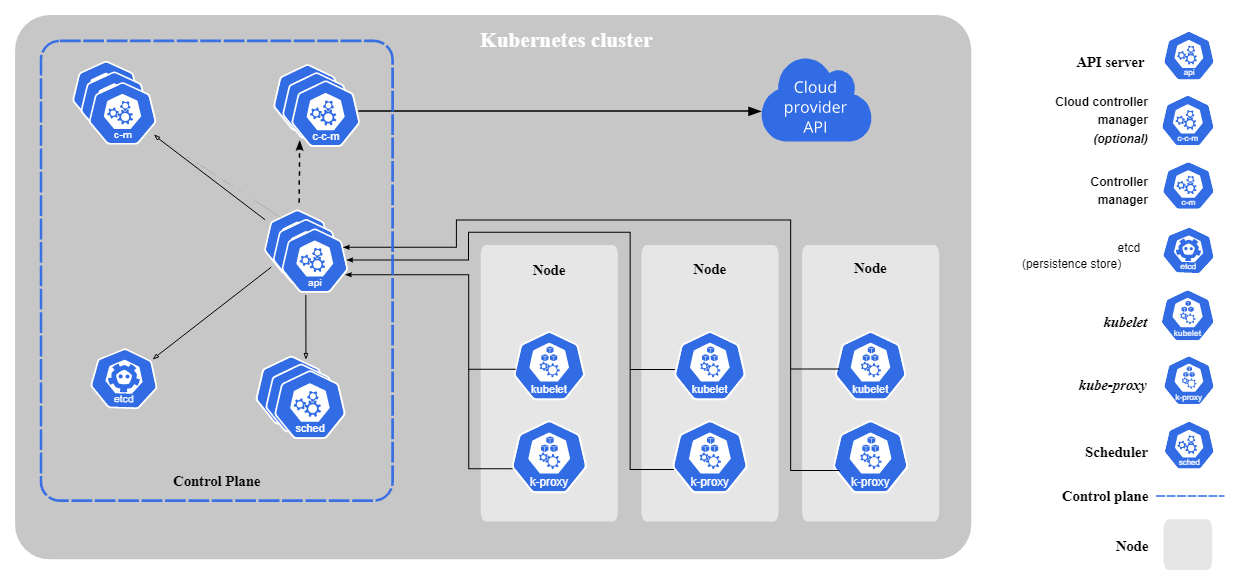
\includegraphics[width=0.7\linewidth]{Pics/kube-architecture}
					\caption{Kiến trúc của Kubernetes}
					\label{fig:kube-architecture}
				\end{figure}
			
				Các thành phần của cụm Kubernetes:\\
				
				\begin{itemize}				
					\item Control Plane: Là trung tâm điều khiển các cụm và làm các cụm kubernetes hoạt động. Đây là nơi quản lý, lên kế hoạch, lập lịch và theo dõi các pod, các node.
					\item Worker Node: Là một máy ảo hoặc máy vật lý chạy Kubernetes. Đây là nơi container thực sự được triển khai để chạy các ứng dụng.
				\end{itemize}
			
				{\hspace{0.3cm}Các thành phần của Control Plane:\\}
				
				\begin{itemize}				
					\item Kubernetes API server: Nơi mà các quản trị viên và các thành phần khác của Control Plane giao tiếp với nhau.
					\item Scheduler: lập lịch cho các ứng dụng của bạn (chỉ định các workload ví dụ như pods được triển khai ở worker node nào)
					\item  Controller Manager: thực hiện các chức năng cấp cụm, chẳng hạn như nhân bản các thành phần, theo dõi các node, xử lý các node lỗi,...
					\item etcd: một kho dữ liệu phân tán đáng tin cậy lưu trữ cấu hình của các node dưới dạng key value.
				\end{itemize}
			
				{\hspace{0.3cm}Các thành phần của Worker Node:\\}
				
				\begin{itemize}				
					\item kubelet: dùng để giao tiếp với API server và quản lý các container nằm trong node.
					\item kube-proxy: là một proxy chạy trên các node trong  Kubernetes. kube-proxy duy trì các quy tắc mạng trên các nút. Các quy tắc mạng này cho phép các Pods trong cùng một node hoặc khác node có thể giao tiếp với nhau.
					\item container-runtime: có thể là Docker, rkt, containerd hoặc một loại container-runtime khác.
				\end{itemize}
			
			\subsection{Tổng quan về Pod}
				{\hspace{0.6cm}Pod là đơn vị thực thi cơ bản của 1 ứng dụng Kubernetes, là đơn vị nhỏ nhất và đơn giản nhất trong mô hình object của Kubernetes. Một Pod đại diện cho các process (tiến trình) chạy trên cluster.\\}
				
				Pod đóng gói một container của ứng dụng (hoặc trong một số trường hợp là nhiều container), tài nguyên lưu trữ, một định danh network duy nhất (địa chỉ IP) cũng như các tùy chọn chi phối cách thức các container sẽ chạy. Một Pod đại diện cho một đơn vị triển khai: một instance (phiên bản) của một ứng dụng trong Kubernetes, có thể chứa một container hoặc vài container được liên kết chặt chẽ và chia sẻ tài nguyên.\\
				
				Docker là container runtime phổ biến nhất được sử dụng cho Pod trong Kubernetes, tuy nhiên Pods cũng hỗ trợ các container runtime khác.\\
				
				Pod trong Kubernetes cluster có thể được sử dụng theo hai cách chính:\\
				\begin{itemize}				
					\item Pods chạy một container duy nhất. Mô hình “một-container-một-Pod” là trường hợp sử dụng phổ biến nhất của Kubernetes; trong trường hợp này, ta có thể nghĩ về một Pod như một trình bao bọc (đóng gói) xung quanh một container và Kubernetes quản lý các Pod thay vì quản lý trực tiếp các container.
					\item Pods chạy nhiều container cần tương tác với nhau. Một Pod có thể đóng gói một ứng dụng chứa nhiều container cùng hoạt động và được liên kết chặt chẽ với nhau cũng như cần chia sẻ tài nguyên (được gọi là co-located container). Các co-located container này có thể tạo thành một đơn vị dịch vụ gắn kết duy nhất nghĩa là 1 container phục vụ các file từ một volume chia sẻ cho public, trong khi đó, một “sidecar” container khác sẽ làm mới (refresh) hoặc cập nhật các file đó. Pod đóng gói các container và tài nguyên lưu trữ này lại với nhau như một thực thể có thể quản lý được.
				\end{itemize}
			\subsection{Vòng đời của Pod}
				{\hspace{0.6cm}Giống như các container, Pod được coi là các thực thể tạm bợ, không bền vững(thay vì lâu bền). Các Pod được tạo, gán một ID (UID) duy nhất và được lên lịch cho các node mà chúng vẫn duy trì cho đến khi bị hủy bỏ (theo chính sách khởi động lại) hoặc xóa. Nếu một node chết, các Pod được lập lịch cho node đó sẽ được lập lịch để xóa sau một khoảng thời gian chờ.\\}
				
				Pod không tự chữa lành. Nếu một Pod được lên lịch cho một node sau đó không thành công, Pod đó sẽ bị xóa; tương tự như vậy, một Pod sẽ không tồn tại sau khi bị trục xuất do thiếu tài nguyên hoặc bảo trì Node. Kubernetes sử dụng phần trừu tượng cấp cao hơn, được gọi là bộ điều khiển, xử lý công việc quản lý các cá thể Pod tương đối dùng một lần.\\
				
				Một Pod nhất định (như được xác định bởi UID) không bao giờ được "lên lịch" đến một nút khác; thay vào đó, Pod đó có thể được thay thế bằng một Pod mới, gần giống, thậm chí có cùng tên nếu muốn, nhưng với một UID khác.\\
				
				Giai đoạn của Pod là một bản tóm tắt đơn giản về vị trí của Pod trong vòng đời của nó.Các giai đoạn của Pod:
				\begin{itemize}				
					\item Pending: Pod đã được chấp nhận bởi hệ thống kubernetes, nhưng 1 hoặc vài container image chưa được tạo ra. Nó bao gồm thời gian trước khi được lập lịch cũng như thời gian download image trên mạng về (có thể mất một lúc)
					\item Running: Pod đã được đưa vào 1 node và tất cả các container đã được tạo ra. Ít nhất 1 container vẫn đang chạy hoặc đang ở trong quá trình bắt đầu hoặc khởi động lại.
					\item  Succeeded: Tất cả các container trong pod đã kết thúc thành công và sẽ không được khởi động lại nữa.
					\item  Failed: Tất cả các container trong pod đã kết thúc và ít nhất 1 contrainer đã thất bại trong quá trình kết thúc. Có nghĩa là container đã exited (thoát) với trạng thái non-zero hoặc đã bị kết thúc bởi hệ thống.
					\item  Unknown: Vì một số lý do, trạng thái của pod không thể xác định được, thường là do bị lỗi trong việc giao tiếp với host của pod.
				\end{itemize}
			\subsection{Quản lí pod bằng Workload trên Kubernetes}
				{\hspace{0.6cm}Workload là một ứng dụng chạy trên Kubernetes. Cho dù workload là một thành phần đơn lẻ hay nhiều thành phần hoạt động cùng nhau, trên Kubernetes, chúng chạy bên trong một tập hợp các pod. Trong Kubernetes, Pod đại diện cho một tập hợp các container đang chạy trên cụm của bạn.\\}
				
				Các Pod có một vòng đời xác định. Ví dụ: khi một Pod đang chạy trong cụm thì một lỗi nghiêm trọng trên node nơi pod đó đang chạy có nghĩa là tất cả các pod trên node đó đều bị lỗi. Kubernetes coi mức độ thất bại đó là cuối cùng: bạn sẽ cần tạo một Pod mới để khôi phục, ngay cả khi node sau đó trở lại bình thường.\\
				
				Tuy nhiên, để làm cho công việc dễ dàng hơn, chúng ta không cần phải quản lý trực tiếp từng Pod. Thay vào đó, bạn có thể sử dụng các workload để quản lý một nhóm các Pod. Các tài nguyên này định cấu hình bộ điều khiển để đảm bảo số lượng phù hợp của loại Pod phù hợp đang chạy, phù hợp với trạng thái chúng ta đã cấu hình.\\
				
				Kubernetes cung cấp một số workload tích hợp sẵn:
				\begin{itemize}				
					\item Deployment và ReplicaSet (thay thế cho ReplicationController). Deployment rất phù hợp để quản lý workload không trạng thái trên cụm, nơi bất kỳ Pod nào trong Deployment đều có thể hoán đổi cho nhau và có thể được thay thế nếu cần.
					\item StatefulSet là workload API object được dùng để quản lý các ứng dụng stateful (có trạng thái). Nó quản lý việc triển khai và co giãn (scale) các pod và cung cấp sự đảm bảo về thứ tự và tính duy nhất của các pod này.
					\item  Một DeamonSet đảm bảo rằng tất cả hoặc một vài node sẽ chạy 1 bản sao của pod. Khi các node được thêm vào cluster thì pod sẽ được lập lịch vào chúng.
					\item  Job và CronJob xác định các nhiệm vụ chạy đến khi hoàn thành và sau đó dừng lại. Công việc đại diện cho các nhiệm vụ một lần, trong khi CronJobs lặp lại theo lịch trình.
				\end{itemize}
	\section{Một số vấn đề bảo mật kiến trúc Microservices}
			{\hspace{0.6cm}Trong hầu hết các ứng dụng được xây dựng trên cấu trúc monolith, bảo mật được thực thi tập trung và các thành phần riêng lẻ không cần phải lo lắng về việc thực hiện các kiểm tra bảo mật trừ khi có yêu cầu. Kết quả là, mô hình bảo mật của một ứng dụng dựa trên cấu trúc monolith là đơn giản hơn nhiều so với ứng dụng được xây dựng dựa trên cấu trúc microservices. Sau đây là một số vấn đề về bảo mật của kiến trúc Microservices gặp phải.\\}			
		\subsection{Càng nhiều microservices thì nguy cơ bị tấn công càng cao}
				{\hspace{0.6cm}Trong một ứng dụng được xây dựng trên cấu trúc monolith, giao tiếp giữa các thành phần bên trong xảy ra trong một tiến trình duy nhất — ví dụ: trong một ứng dụng Java, trong cùng một Máy ảo Java (JVM). Theo kiến trúc microservices, các thành phần bên trong đó được thiết kế dưới dạng các microservices riêng biệt, độc lập và các tiến trình phải gọi lẫn nhau để trao đổi các thông tin. Ngoài ra, mỗi microservice hiện chấp nhận các request một cách độc lập hoặc có các điểm truy cập riêng. Thay vì một vài điểm truy cập, như trong một ứng dụng xây dựng trên cấu trúc monolith, bây giờ chúng ta có số lượng lớn các điểm truy cập. Khi số lượng truy cập vào hệ thống tăng lên, chúng ta sẽ có nhiều điểm bị tấn công hơn. Vấn đề này là một trong những thách thức cơ bản trong việc xây dựng thiết kế bảo mật cho microservices.\\}
		\subsection{Kiểm tra bảo mật phân tán có thể dẫn đến hiệu suất giảm}
				{\hspace{0.6cm}Không giống như trong một ứng dụng được xây dựng trên cấu trúc monolith, mỗi microservice trong triển khai microservices phải thực hiện kiểm tra an ninh độc lập. Từ quan điểm của một ứng dụng dựa trên cấu trúc monolith, trong đó việc kiểm tra bảo mật được thực hiện một lần và các request được gửi đến thành phần tương ứng, nhưng đối với các microservice chúng ta phải kiểm tra tất các các điểm truy cập của chúng. Ngoài ra, trong khi xác thực các yêu cầu tại mỗi microservice, bạn có thể cần kết nối với dịch vụ mã thông báo bảo mật từ xa (STS). Các kiểm tra bảo mật phân tán, lặp đi lặp lại và kết nối từ xa này có thể làm tăng độ trễ và làm giảm đáng kể hiệu suất của hệ thống.\\}
				
				Một số giải quyết vấn đề này bằng cách đơn giản là tin tưởng vào mạng và tránh kiểm tra bảo mật các microservice. Theo thời gian, mạng tin cậy đã trở thành lỗi thời và đang tiến tới các nguyên tắc mạng không tin cậy. Với nguyên tắc mạng không tin cậy, chúng ta thực hiện bảo mật với từng tài nguyên trong mạng. Mọi thiết kế bảo mật microservices phải có hiệu suất tổng thể có thể chấp nhận được.
		\subsection{Sự phức tạp khi triển khai xác thực khởi động giữa các	microservices}
				{\hspace{0.6cm}Giao tiếp dịch vụ với dịch vụ diễn ra giữa các microservice. Mỗi kênh liên lạc giữa các microservice phải được bảo vệ. Chúng có nhiều tùy chọn, nhưng giả sử rằng chúng ta sử dụng chứng chỉ (certificates).\\}
				
				Giờ đây, mỗi microservice phải được cấp chứng chỉ (và khóa bí mật tương ứng), chứng chỉ này sẽ sử dụng để xác thực chính nó với một microservice khác trong quá trình tương tác giữa dịch vụ với dịch vụ. Microservice của người nhận phải biết cách xác thực chứng chỉ được liên kết với microservice đang gọi. Do đó cần một cách để tin tưởng bootstrap giữa các microservices. Ngoài ra cần có khả năng thu hồi chứng chỉ (trong trường hợp khóa bí mật tương ứng bị xâm phạm) và cấp các chứng chỉ mới (thay đổi chứng chỉ định kỳ để giảm thiểu mọi rủi ro khi vô tình làm mất chìa khóa). Những tác vụ này rất cồng kềnh và trừ khi chúng ta tìm ra cách tự động hóa chúng.\\
		\subsection{Khó theo dõi các request của các microservice}
				{\hspace{0.6cm}Khả năng giám sát là thước đo những gì có thể suy ra về trạng thái bên trong của một hệ thống dựa trên kết quả đầu ra bên ngoài của nó. Nhật ký (logs), chỉ số (metrics) và dấu vết (traces) được coi là ba trụ cột của khả năng giám sát.\\}
				
				Nhật ký có thể là bất kỳ sự kiện nào bạn ghi lại tương ứng với một dịch vụ nhất định.\\
				
				Tổng hợp một tập hợp các nhật ký có thể tạo ra các chỉ số. Theo một cách nào đó, các chỉ số phản ánh trạng thái hệ thống. Ví dụ về mặt bảo mật, các yêu cầu truy cập không hợp lệ trung bình mỗi giờ là một chỉ số.\\
				
				Dấu vết cũng dựa trên nhật ký nhưng cung cấp một góc nhìn khác về hệ thống. Theo dõi giúp bạn theo dõi một yêu cầu từ điểm mà nó đi vào hệ thống đến chỉ nơi nó rời khỏi hệ thống. Quá trình này trở nên khó khăn trong mô hình microservices. Không giống như trong một ứng dụng theo cấu trúc monolith, một yêu cầu triển khai microservices có thể xâm nhập vào hệ thống thông qua một microservice và trải dài trên nhiều microservices trước khi nó rời khỏi hệ thống.			
		\subsection{Tính bất biến của container làm việc xác thực và chính sách kiểm soát truy cập của các dịch vụ khó khăn}
				{\hspace{0.6cm}Máy chủ không thay đổi trạng thái sau khi quay được gọi là máy chủ bất biến. Các mô hình triển khai phổ biến nhất cho microservices là dựa trên container. Mỗi microservice chạy bằng container riêng của nó và tất nhiên, container phải là một máy chủ bất biến. Nói cách khác, sau khi container khởi động, nó sẽ không thay đổi bất kỳ tệp nào trong hệ thống tệp của nó hoặc duy trì bất kỳ trạng thái của nó không thay đổi lúc nó đang chạy.\\}
				
				Tính bất biến có tác động gì đến bảo mật và tại sao khái niệm máy chủ bất biến lại được coi là thách thức bảo mật microservices? Trong kiến trúc bảo mật microservices, mỗi microservice trở thành một điểm cần được bảo mật. Do đó, cần duy trì danh sách các máy khách được phép (có thể là các microservice khác) có thể truy cập vào microservice này và cần một bộ chính sách kiểm soát truy cập. Những danh sách này không tĩnh; chúng ta cần được phép cập nhật các danh sách này. Nhưng với tính chất bất biến của container, chúng ta không thể update hệ thống tệp trong các container của các microservice.
		\subsection{Kiến trúc đa ngôn ngữ đòi hỏi các developer phải có thêm nhiều kiến thức bảo mật hơn}
				{\hspace{0.6cm}Trong triển khai microservices, các dịch vụ nói chuyện với nhau qua mạng. Họ không phụ thuộc vào việc triển khai từng dịch vụ, mà phụ thuộc vào giao diện dịch vụ. Tình huống này cho phép mỗi microservice chọn ngôn ngữ lập trình của riêng mình và nền tảng công nghệ để triển khai. Trong một môi trường, trong đó mỗi đội development triển khai các mircoservice của riêng mình, mỗi nhóm có thể linh hoạt để chọn các stack công nghệ để phù hợp với sản phẩm. Kiến trúc này, cho phép các các thành phần trong hệ thống để chọn công nghệ tốt nhất cho chúng, được gọi là một kiến trúc đa ngôn ngữ.\\}
				
				Một kiến trúc đa ngôn ngữ làm cho vấn đề bảo mật trở nên khó khăn. Bởi vì các đội khác nhau sử dụng các stack công nghệ khác nhau để phát triển, mỗi nhóm phải có các chuyên gia bảo mật riêng. Các chuyên gia này phải chịu trách nhiệm xác định các phương pháp bảo mật tốt nhất và hướng dẫn, nghiên cứu các công cụ bảo mật cho mỗi stack công nghệ để phân tích mã nguồn tĩnh và thử nghiệm động và tích hợp các công cụ đó vào quá trình xây dựng. Trách nhiệm của một nhóm bảo mật tập trung, nhưng bây giờ chia vào các đội development. Điều này làm cho các đội development không chú tâm vào việc phát triển sản phẩm mà phải lo một phần về bảo mật nữa làm cho chất lượng sản phẩm giảm do phải viết các module bảo mật làm cho mã nguồn bị rối và khó đọc.
				
	\newpage				
	\section*{Kết luận Chương 1}
			\hspace{0.6cm}Như vậy trong chương một nhóm đã nêu ra những thông tin cơ về những công nghệ cũng như kiến trúc của tương lai - Container và Microservices. Đưa ra những ưu điểm cũng như thách thức trong việc triển khai, sử dụng những công nghệ này trong thực tế. Đồng thời nhóm cũng nêu ra một hệ thống tự động hoá triển khai, mở rộng và quản lý của công nghệ Container là Kubernetes. Qua việc hiểu tổng quan của các công nghệ trên nhóm đã nhận ra một số vấn đề bảo mật của kiến trúc Microservices như nguy cơ bị tấn công cao khi mở rộng, việc ảnh hưởng đến hiệu suất khi triển khai bảo mật phân tán cũng như sự phức tạp, khó khăn khi triển khai các giải pháp an toàn cũng yêu cầu nhiều kiến thức đối với những nhà phát triển. Sau đây nhóm sẽ trình bày một giải pháp để có thể giải quyết những vấn đề nói trên.
\chapter{Tổng quan về Istio}
	\section{Tổng quan về Istio}
		\subsection{Tổng quan về Service Mesh}
			\hspace{0.6cm}Kiến trúc Microservice ngày càng trở nên phổ biến và trở thành lựa chọn hàng đầu trong quá trình phát triển phần mềm. Trong kiến trúc microservice, ứng dụng monolithic truyền thống được chia nhỏ ra thành các thành phần có thể deploy độc lập. Một ứng dụng dần trở thành một nhóm các service, khi bạn có hàng trăm, hàng ngàn các service nhỏ cùng hoạt động, một bài toán mới về vấn đề giao tiếp giữa các service cần được giải quyết.\\
			
			Giả sử chúng ta có website bán hàng online được triển khai theo kiến trúc microservice, chúng ta sẽ có:
			\begin{itemize}
				\item Web server service: xử lý các request về UI
				\item Payment service: xử lý các request về thanh toán
				\item Shopping cart service: xử lý các request về giỏ hàng
				\item Product inventory service: xử lý các request về kho hàng
				\item Database service
				\item ..., rất nhiều các microservice xử lý các vấn đề khác nữa
			\end{itemize}
		
		Khi chúng ta deploy website trong Kubernetes cluster, để website hoạt động ổn định, trước tiên các service cần hoạt động chính xác, web server cần xử lý chính xác business logic, database cần lưu đầy đủ thông tin,... hơn hết các service cần giao tiếp thông suốt với nhau. Khi user gửi 1 request thêm sản phẩm vào giỏ hàng lên web server, web server cần thông báo sang cho shopping cart service, rồi lưu thông tin đó vào database. Vì vậy, các service cần phải biết làm thế nào để giao tiếp với các service khác, đâu là đích đến tiếp theo của request, địa chỉ endpoint của từng service, để web server biết phải giao tiếp với endpoint nào chúng ta cần cấu hình cho nó. Khi ta scale ứng dụng lên và có nhiều thêm các microservice, chúng ta lại config endpoint cho tất cả các service đã hoạt động trước đó. Cấu hình địa chỉ endpoint trở thành 1 phần không thể tách rời của các service.
		
		\newpage Nói về vấn đề security, ứng dụng dùng kiến trúc microservice trông sẽ như này:
		\begin{figure}[h]
			\centering
			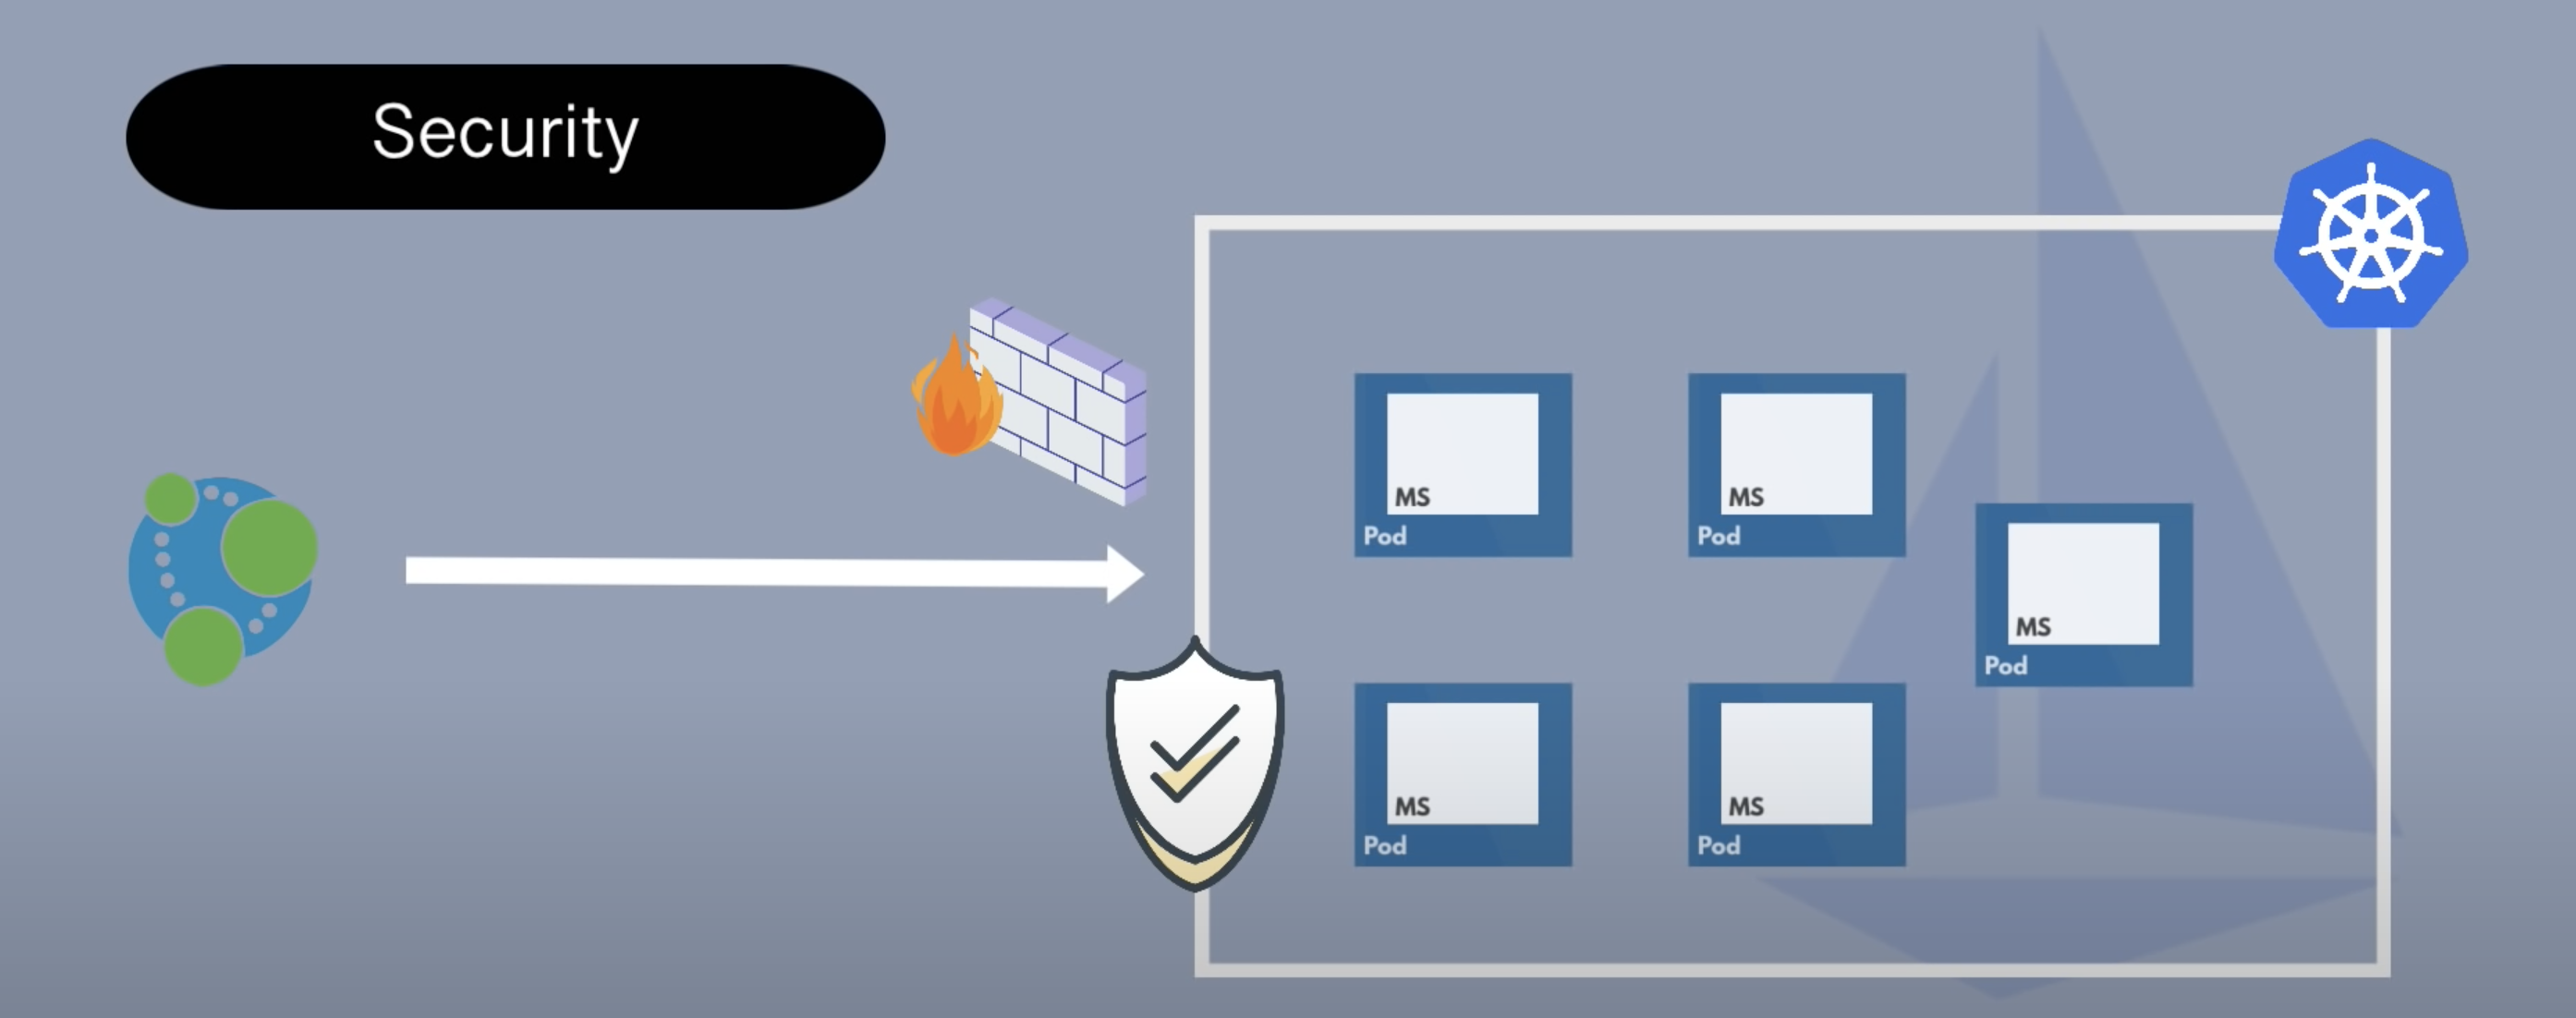
\includegraphics[width=0.7\linewidth]{Pics/2.1.1-p1}
			\caption{Ứng dụng kiến trúc Microservices trong Security}
			\label{fig:2.1.1-1}
		\end{figure}
		
		Chúng ta có firewall hoặc proxy để tránh Kubernetes cluster được truy cập trực tiếp, bảo vệ cho các dịch vụ bên trong cluster. Tuy nhiên ngay khi yêu cầu đi vào bên trong cluster, các dịch vụ giao tiếp với nhau 1 cách kém bảo mật, chúng giao tiếp với nhau thông qua http hoặc protocol kém bảo mật hơn, các dịch vụ giao tiếp tự do với nhau bên trong cluster - nơi không được bảo mật nữa. Khi ai đó tấn công vào ứng dụng, vượt qua firewall/proxy để vào bên trong cluster, họ thoải mái làm mọi thứ, có thể lấy các thông tin nhạy cảm của người dùng. Vì vậy chúng ta bổ sung thêm các security logic cho dịch vụ để đảm bảo việc giao tiếp giữa các dịch vụ bên trong cluster được an toàn.
		
		Mỗi dịch vụ cũng cần được bổ sung khả năng khởi động lại để khi dịch vụ không thể truy cập, hoặc các dịch vụ khác mất kết nối, tự nó có thể khởi động lại, để đảm bảo giao tiếp thông suốt.
		
		Ngoài ra, bạn cũng cần giám sát cách hoạt động của dịch vụ, cần nắm được các thông số về thời gian dịch vụ xử lý một yêu cầu, số lượng yêu cầu/phản hồi của mỗi dịch vụ. Cuối cùng mỗi dịch vụ sẽ được bổ sung thêm rất nhiều các logic bên cạnh business logic của dịch vụ rồi các nhà phát triển sẽ không còn tập trung vào phát triển logic cho dịch vụ mà còn phải xử lý cả các logic về mạng cho metrics, security, communication,... Điều này khiến các dịch vụ trở nên phức tạp và không còn đơn giản, gọn nhẹ như mục tiêu của microservice nữa.
		\begin{figure}[h]
			\centering
			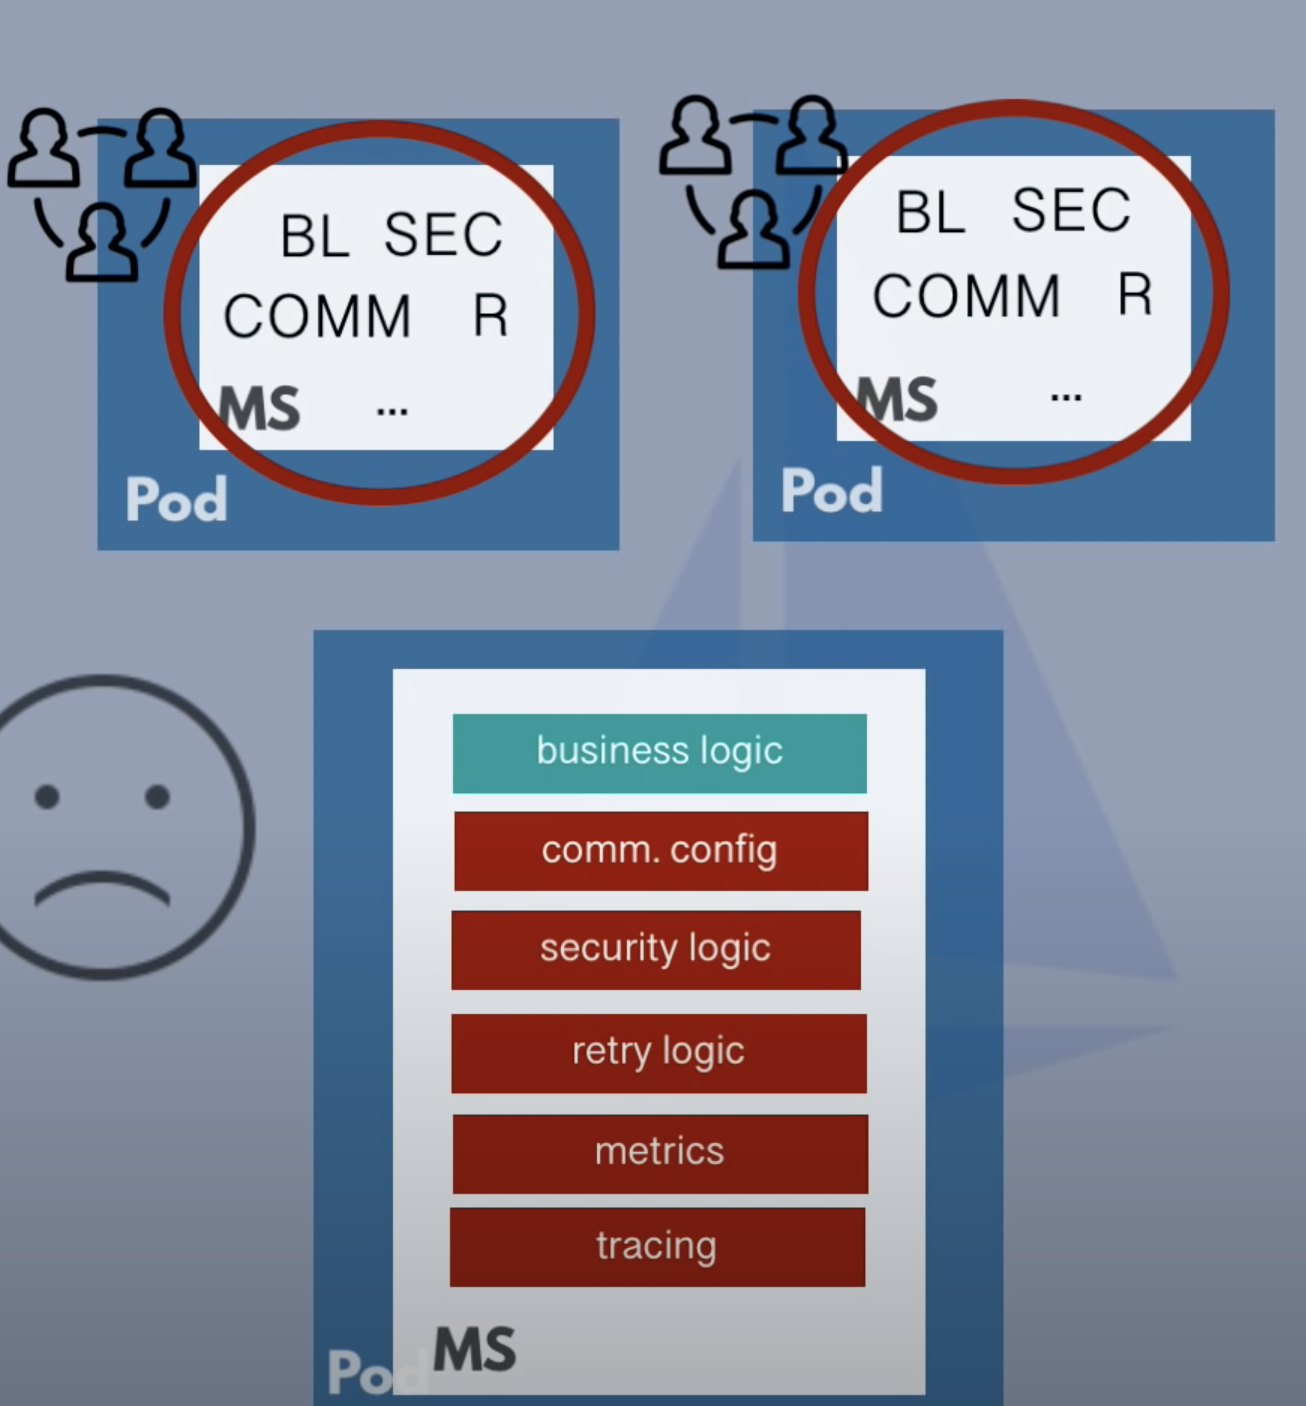
\includegraphics[width=0.48\linewidth]{Pics/2.1.1-p2}
			\caption{Các vấn đề gặp phải}
			\label{fig:2.1.1-2}
		\end{figure}
		
		Để giải quyết vấn đề này, chúng ta cần tách biệt các non-business logic với business logic khỏi service bằng solution được gọi là Service Mesh.
		
		Service Mesh là lớp cơ sở hạ tầng chuyên dụng kiểm soát giao tiếp qua mạng giữa dịch vụ với dịch vụ. Service Mesh cho phép các phần riêng biệt của ứng dụng giao tiếp với nhau. Service Mesh xuất hiện phổ biến cùng với các ứng dụng, bộ chứa và vi dịch vụ dựa trên đám mây.
		
		Service Mesh kiểm soát việc cung cấp các yêu cầu dịch vụ trong một ứng dụng. Service Mesh cung cấp các tính năng phổ biến gồm khám phá dịch vụ, cân bằng tải,mã hóa và khôi phục lỗi. Thay vì thông qua phần cứng, tính sẵn sàng cao cũng phổ biến thông qua việc sử dụng phần mềm được kiểm soát bởi API. Service Mesh có thể giúp giao tiếp giữa dịch vụ với dịch vụ nhanh chóng, đáng tin cậy và an toàn.
		
		Một tổ chức có thể chọn cổng API xử lý các giao dịch giao thức thay Service Mesh. Dù vậy, các nhà phát triển phải cập nhật cổng API mỗi khi thêm hoặc xóa một vi dịch vụ. Khả năng mở rộng quản lý mạng và tính linh hoạt của Service Mesh thường vượt trội so với khả năng của các cổng API truyền thống.
		
		\subsubsection{Cách thức hoạt động của Service Mesh}
		\hspace{0.6cm}Trong bất kỳ mô hình phát triển nào đang được sử dụng thì Service Mesh sử dụng một phiên bản proxy được gọi là sidecar. Trong một ứng dụng microservice, một sidecar gắn vào mỗi dịch vụ. Trong một vùng chứa, sidecar gắn vào từng vùng chứa ứng dụng, VM hoặc đơn vị điều phối vùng chứa, chẳng hạn như nhóm Kubernetes. Qua đây các Service Mesh trở thành ứng dụng bên thứ ba và giúp người vận hành cluster có thể cấu hình chúng dễ dàng hơn.
		
		Sidecar có thể xử lý các tác vụ được trừu tượng hóa từ chính dịch vụ, chẳng hạn như giám sát và bảo mật.
		
		Trong Service Mesh sidecar và các tương tác của chúng tạo nên được gọi là data plane. Một lớp khác quản lý các tác vụ như tạo phiên bản, giám sát và triển khai các chính sách để quản lý và bảo mật mạng được gọi là control plane. Các control plane có thể kết nối với CLI hoặc giao diện GUI để quản lý ứng dụng. Nhờ có control plane giúp cho các nhà phát triển không cần đưa Service Mesh vào trong deploy config của microservices.
		
		\subsubsection{Tại sao áp dụng Service Mesh?}
		\hspace{0.6cm}Một ứng dụng được cấu trúc theo kiến trúc microservices có thể chứa hàng chục hoặc hàng trăm dịch vụ, Mỗi dịch vụ đều có các phiên bản riêng hoạt động trong môi trường trực tiếp. Điều này gây khó khăn cho các nhà phát triển khi theo dõi những thành phần nào phải tương tác, theo dõi tình trạng và hiệu suất của chúng cũng như thực hiện các thay đổi đối với dịch vụ hoặc thành phần nếu có sự cố.
		
		Service Mesh cho phép các nhà phát triển tách biệt và quản lý các giao tiếp giữa dịch vụ với dịch vụ trong một lớp cơ sở hạ tầng chuyên dụng. Lợi ích của việc sử dụng Service Mesh càng tăng khi số lượng vi dịch vụ liên quan đến một ứng dụng tăng lên.
		
			\subsubsection{Các tính năng chính của Service Mesh}
		\hspace{0.6cm}Service Mesh thường cung cấp nhiều khả năng giúp quá trình giao tiếp trong vùng chứa và vi dịch vụ trở nên đáng tin cậy, an toàn và dễ quan sát hơn.
		\begin{itemize}
			\item \textbf{Độ tin cậy:} Quản lý thông tin liên lạc thông qua proxy sidecar và control plane cải thiện hiệu quả và độ tin cậy của các yêu cầu dịch vụ, chính sách và cấu hình. Các khả năng cụ thể bao gồm cân bằng tải và tiêm lỗi.
			\item \textbf{Khả năng quan sát:} Service Mesh có thể cung cấp thông tin chi tiết về hành vi và tình trạng của dịch vụ. Control plane có thể thu thập và tổng hợp dữ liệu đo từ xa từ các tương tác thành phần nhằm xác định tình trạng dịch vụ, chẳng hạn như lưu lượng truy cập và độ trễ, theo dõi phân tán và nhật ký truy cập. Tích hợp của bên thứ ba với các công cụ, chẳng hạn như Prometheus, Elasticsearch và Grafana, cho phép theo dõi và trực quan hóa hơn nữa.
			\item \textbf{Bảo vệ:} Service Mesh có thể tự động mã hóa thông tin liên lạc và phân phối các chính sách bảo mật, bao gồm xác thực và ủy quyền, từ mạng đến ứng dụng và các dịch vụ nhỏ riêng lẻ. Quản lý tập trung các chính sách bảo mật thông qua control plane và proxy sidecar giúp theo kịp các kết nối ngày càng phức tạp bên trong và giữa các ứng dụng phân tán.
		\end{itemize}
		
			\subsubsection{Lợi ích và hạn chế của Service Mesh}
		\hspace{0.6cm}Service Mesh có một số ưu điểm của như sau:
		\begin{itemize}
			\item Đơn giản hóa giao tiếp giữa các dịch vụ trong cả microservice và container.
			\item Dễ chẩn đoán lỗi giao tiếp hơn vì chúng sẽ xảy ra trên lớp cơ sở hạ tầng của chính chúng.
			\item Hỗ trợ các tính năng bảo mật như mã hóa, xác thực và ủy quyền.
			\item Cho phép phát triển, thử nghiệm và triển khai ứng dụng nhanh hơn.
			\item Sidecars được đặt bên cạnh một cụm container có hiệu quả trong việc quản lý các dịch vụ mạng.
		\end{itemize}
		
		Service Mesh có một số nhược điểm như sau:
		\begin{itemize}
			\item Thời gian chạy các dịch vụ tăng thông qua việc sử dụng Service Mesh.
			\item Trước tiên, mỗi cuộc gọi dịch vụ phải chạy qua proxy sidecar, điều này sẽ bổ sung thêm một bước.
			\item Các Service Mesh không đề cập đến việc tích hợp với các dịch vụ hoặc hệ thống khác cũng như loại định tuyến hoặc ánh xạ chuyển đổi.
			\item Độ phức tạp của quản lý mạng được trừu tượng hóa và tập trung, nhưng không bị loại bỏ. Do đó phải tích hợp Service Mesh vào quy trình công việc và quản lý cấu hình của nó.
		\end{itemize}
		
			\subsubsection{Thực trạng Thị trường Service Mesh}
		\hspace{0.6cm}Theo một cuộc khảo sát được thực hiện vào giữa năm 2020, việc áp dụng Service Mesh vào doanh nghiệp vẫn còn non trẻ và thua xa so với container. Theo khảo sát thì Istio, Linkerd và HashiCorp Consul là những mạng lưới dịch vụ được sử dụng nhiều nhất.
		
		Istio, một Service Mesh mã nguồn mở do Google, IBM và Lyft cung cấp, là một control plane chung ban đầu với mục tiêu cho các triển khai Kubernetes, nhưng các kiến trúc sư có thể sử dụng nó trên nhiều nền tảng.data plane của nó dựa trên các proxy được gọi là Envoy sidecar.
		
		Linkerd, một Service Mesh đa nền tảng, mã nguồn mở khác, được phát triển bởi Buoyant và được xây dựng trên thư viện Finagle của Twitter. Service Mesh này hỗ trợ các nền tảng như Kubernetes, Docker và Amazon ECS.
		
		HashiCorp’s Consul cung cấp khả năng khám phá dịch vụ và Service Mesh để xử lý việc quản lý mạng trong môi trường phân tán. Nó hoạt động với AWS và Microsoft Azure và cũng có sẵn dưới dạng sản phẩm SaaS.
		\subsection{Kiến trúc của Istio}
		\hspace{0.6cm}Service Mesh là 1 pattern và Istio là một trong những ứng dụng implement pattern này. Istio là service mesh độc lập, mã nguồn mở được viết bằng go-lang, một ngôn ngữ khá phổ biến để xây dựng những ứng dụng cloud-native (docker, kubernetes…), cung cấp các nguyên tắc cơ bản, giảm sự phức tạp trong việc quản lý microservice bằng cách cung cấp một cách thống nhất để bảo mật, kết nối và giám sát microservice với nhau. Istio có các API cho phép nó tích hợp vào bất kỳ nền tảng logging nào.
		
			\subsubsection{Kiến trúc của Istio}
		\hspace{0.6cm}Kiến trúc của Istio gồm:
		\begin{itemize}
			\item \textbf{Data Plane:} Istio sử dụng Envoy proxy, chịu trách nhiệm:
			\begin{itemize}
				\item Service Discovery
				\item Load Balancing
				\item Authentication and Authorization
				\item Request Tracing
				\item Traffic Management
				\item Fault Injection
				\item Rate Limiting
				\item Observability
			\end{itemize}
			\item \textbf{Control Plane} của Istio là istiod tiếp nhận các tương tác của DevOps/SysAdmin thông qua Command Line Interface — CLI, chịu trách nhiệm quản lý và truyền các envoy proxy vào service.
		\end{itemize}
		\begin{figure}[h]
			\centering
			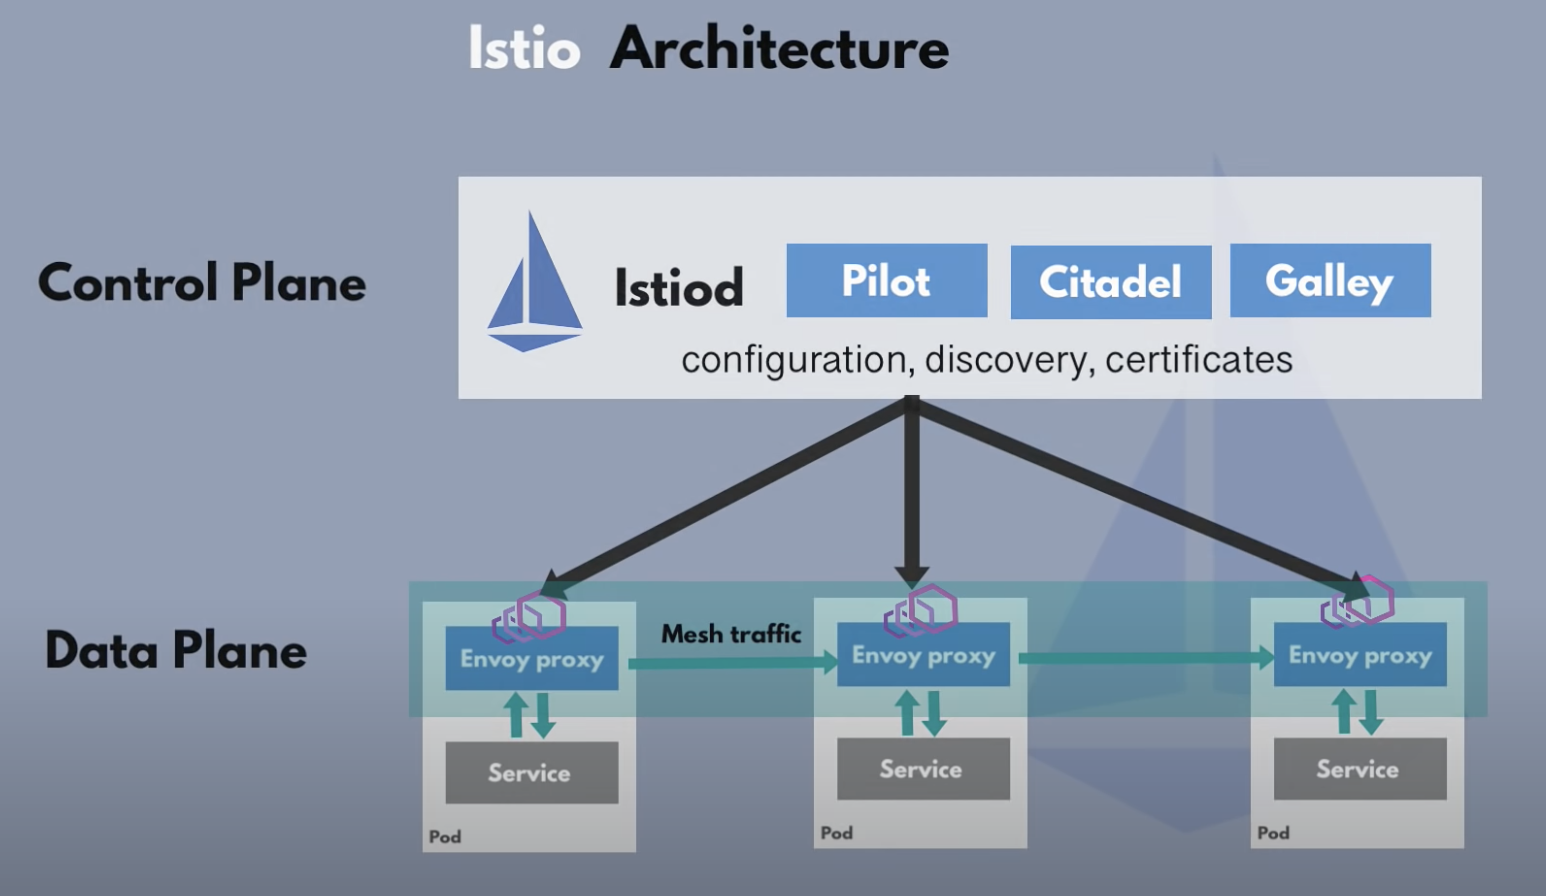
\includegraphics[width=0.7\linewidth]{Pics/2.1.2-p1}
			\caption{Kiến trúc của Istio}
			\label{fig:2.1.2-1}
		\end{figure}
		
		Ở phiên bản 1.5 trở về trước, control plane của Istio được gồm nhiều thành phần như Pilot, Citadel, Galley, Mixer,... mỗi thành phần thì lại được deploy trên Kubernetes như 1 pod riêng biệt. Tuy nhiên từ những version sau, chúng đươc gộp thành một thành phần duy nhất là Istiod, điều này làm cho việc cấu hình và vận hành Istio trở nên dễ dàng hơn.
		
			\subsubsection{Ưu điểm khi sử Istio}
		\hspace{0.6cm}Istio là 1 implementation của Service Mesh, nên tính độc lập của application là một trong những ưu tiên hàng đầu vì thế để đưa các chức năng của Istio vào trong ứng dụng microservice của thì chúng ta không cần thiết phải thay đổi các file cấu hình yaml của các Deployment hay Service, mọi thứ đã được đóng gói trong chính file cấu hình của Istio. Việc cài đặt Istio cũng tách rời với logic của ứng dụng, không làm thay đổi các business logic.
		
		Các component của Istio được kế thừa từ Kubernetes API, dưới dạng CRD, giúp ta dễ dàng cấu hình chúng như cấu hình 1 deployment, service luôn. Istio hỗ trợ cấu hình:
		\begin{itemize}
			\item Traffic routing: cho phép cài đặt nhiều rules khác nhau, quy định các service được giao tiếp với giao nhau.
			\item Traffice split
			\item Retry rule, timeout
		\end{itemize}
		
		Hai CRD chính của Istio là VirtualService định tuyến traffic tới 1 service, khi lưu lượng đã được định tuyến tới dịch vụ, chúng ta có thể sử dụng DestinationRule để cấu hình các chính sách lên nó.
		
		Khi chúng ta tạo các CRD trên Kubernetes, istiod - control plane của Istio, sẽ chuyển đổi chúng thành cấu hình của Envoy và gửi tất cả các cấu hình đó tới các Envoy Proxy sidecar. Khi các Envoy Proxy đã có được cấu hình, chúng sẽ giao tiếp với nhau (không thông qua istiod) dưới các rule mà chúng ta đã dinh nghĩa.
		
		Ngoài việc rất dễ dàng cấu hình Istio, nó còn mang tới những ưu điểm như:
		\begin{itemize}
			\item \textbf{Service discovery: Istio} có 1 central registry cho tất các microservice và các endpoint, không cần phải thêm các cài đặt cho endpoint mỗi microservice, mỗi khi có thêm 1 microservice mới được deploy, nó sẽ được đăng ký 1 các tự động với central registry của Istio
			\item \textbf{Istiod} cũng có thể quản lý các certificates, istiod đóng vai trò như 1 certificate authority, tạo ra certificate cho tất cả các dịch vụ trong cluster, cho phép các dịch vụ giao tiếp bảo mật hơn thông qua kết nối bảo mật TSL.
			\item \textbf{Istio} cũng thu thập dữ liệu từ xa thông qua các Envoy Proxy.
		\end{itemize}
		
			\subsubsection{Luồng traffic sau khi cài đặt Istio}
		\hspace{0.6cm}Ngoài 2 CRD là VirtualService và DestinationRule, Gateway đóng vai trò là 1 entrypoint cho các request từ cluster tới microservice application, nó hoạt động tương tự như Nginx Ingress Controller, đảm nhiệm việc cân bằng tải, điều hướng traffic tới các microservice bằng cấu hình của VirtualService.
		\begin{figure}[h]
			\centering
			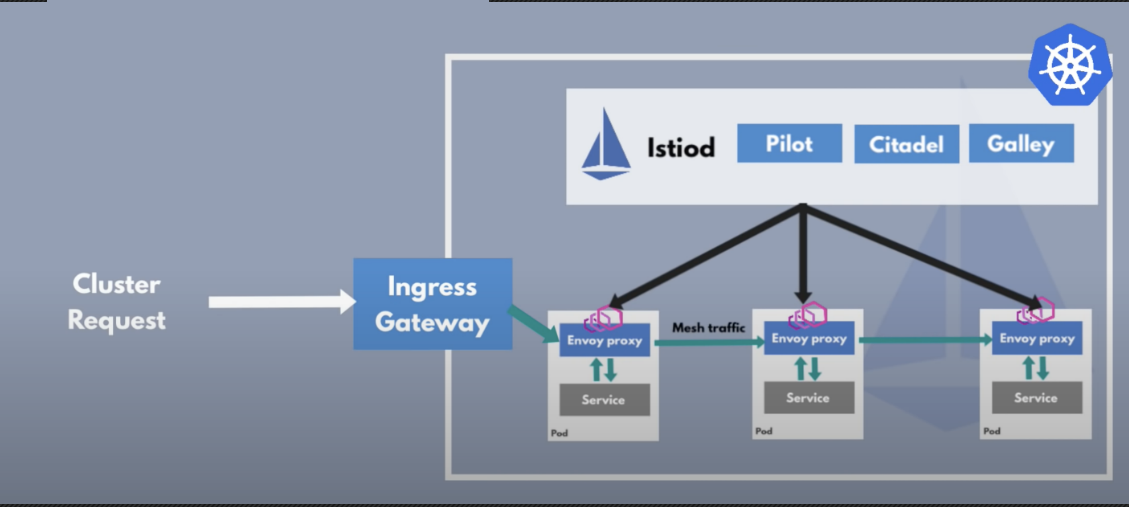
\includegraphics[width=0.7\linewidth]{Pics/2.1.2-p2}
			\caption{Luồng dữ liệu sau khi cài đặt Istio}
			\label{fig:2.1.2-2}
		\end{figure}
		
		\newpage Với ví dụ một trang web bán hàng online, lưu lượng sau khi ứng dụng được cài đặt thêm Istio sẽ như sau: User gửi yêu cầu tới web server service trong Kubernetes, đầu tiên nó sẽ tới Istio Gateway, gateway sẽ tìm ra dịch vụ dựa vào VirtualService rule, và gửi yêu cầu tới dịch vụ web server, cuối cùng yêu cầu sẽ tới Envoy proxy bên trong dịch vụ và được chuyển tiếp tới web server container thông qua localhost. Từ dịch vụ web server, tiếp tục tạo 1 yêu cầu tới dịch vụ thanh toán, yêu cầu sẽ đi từ dịch vụ web server qua Envoy proxy của dịch vụ web server, chúng sẽ được so sánh với các rule của VirtualService và DestinationRule rồi mới tới Envoy proxy của dịch vụ thanh toán, giao tiếp giữa Envoy proxy của web server và payment là mutual TLS. Quá trình này được lặp lại trên các dịch vụ tiếp theo mà yêu cầu gửi đến cho tới khi phản hồi về UI.
		\begin{figure}[h]
			\centering
			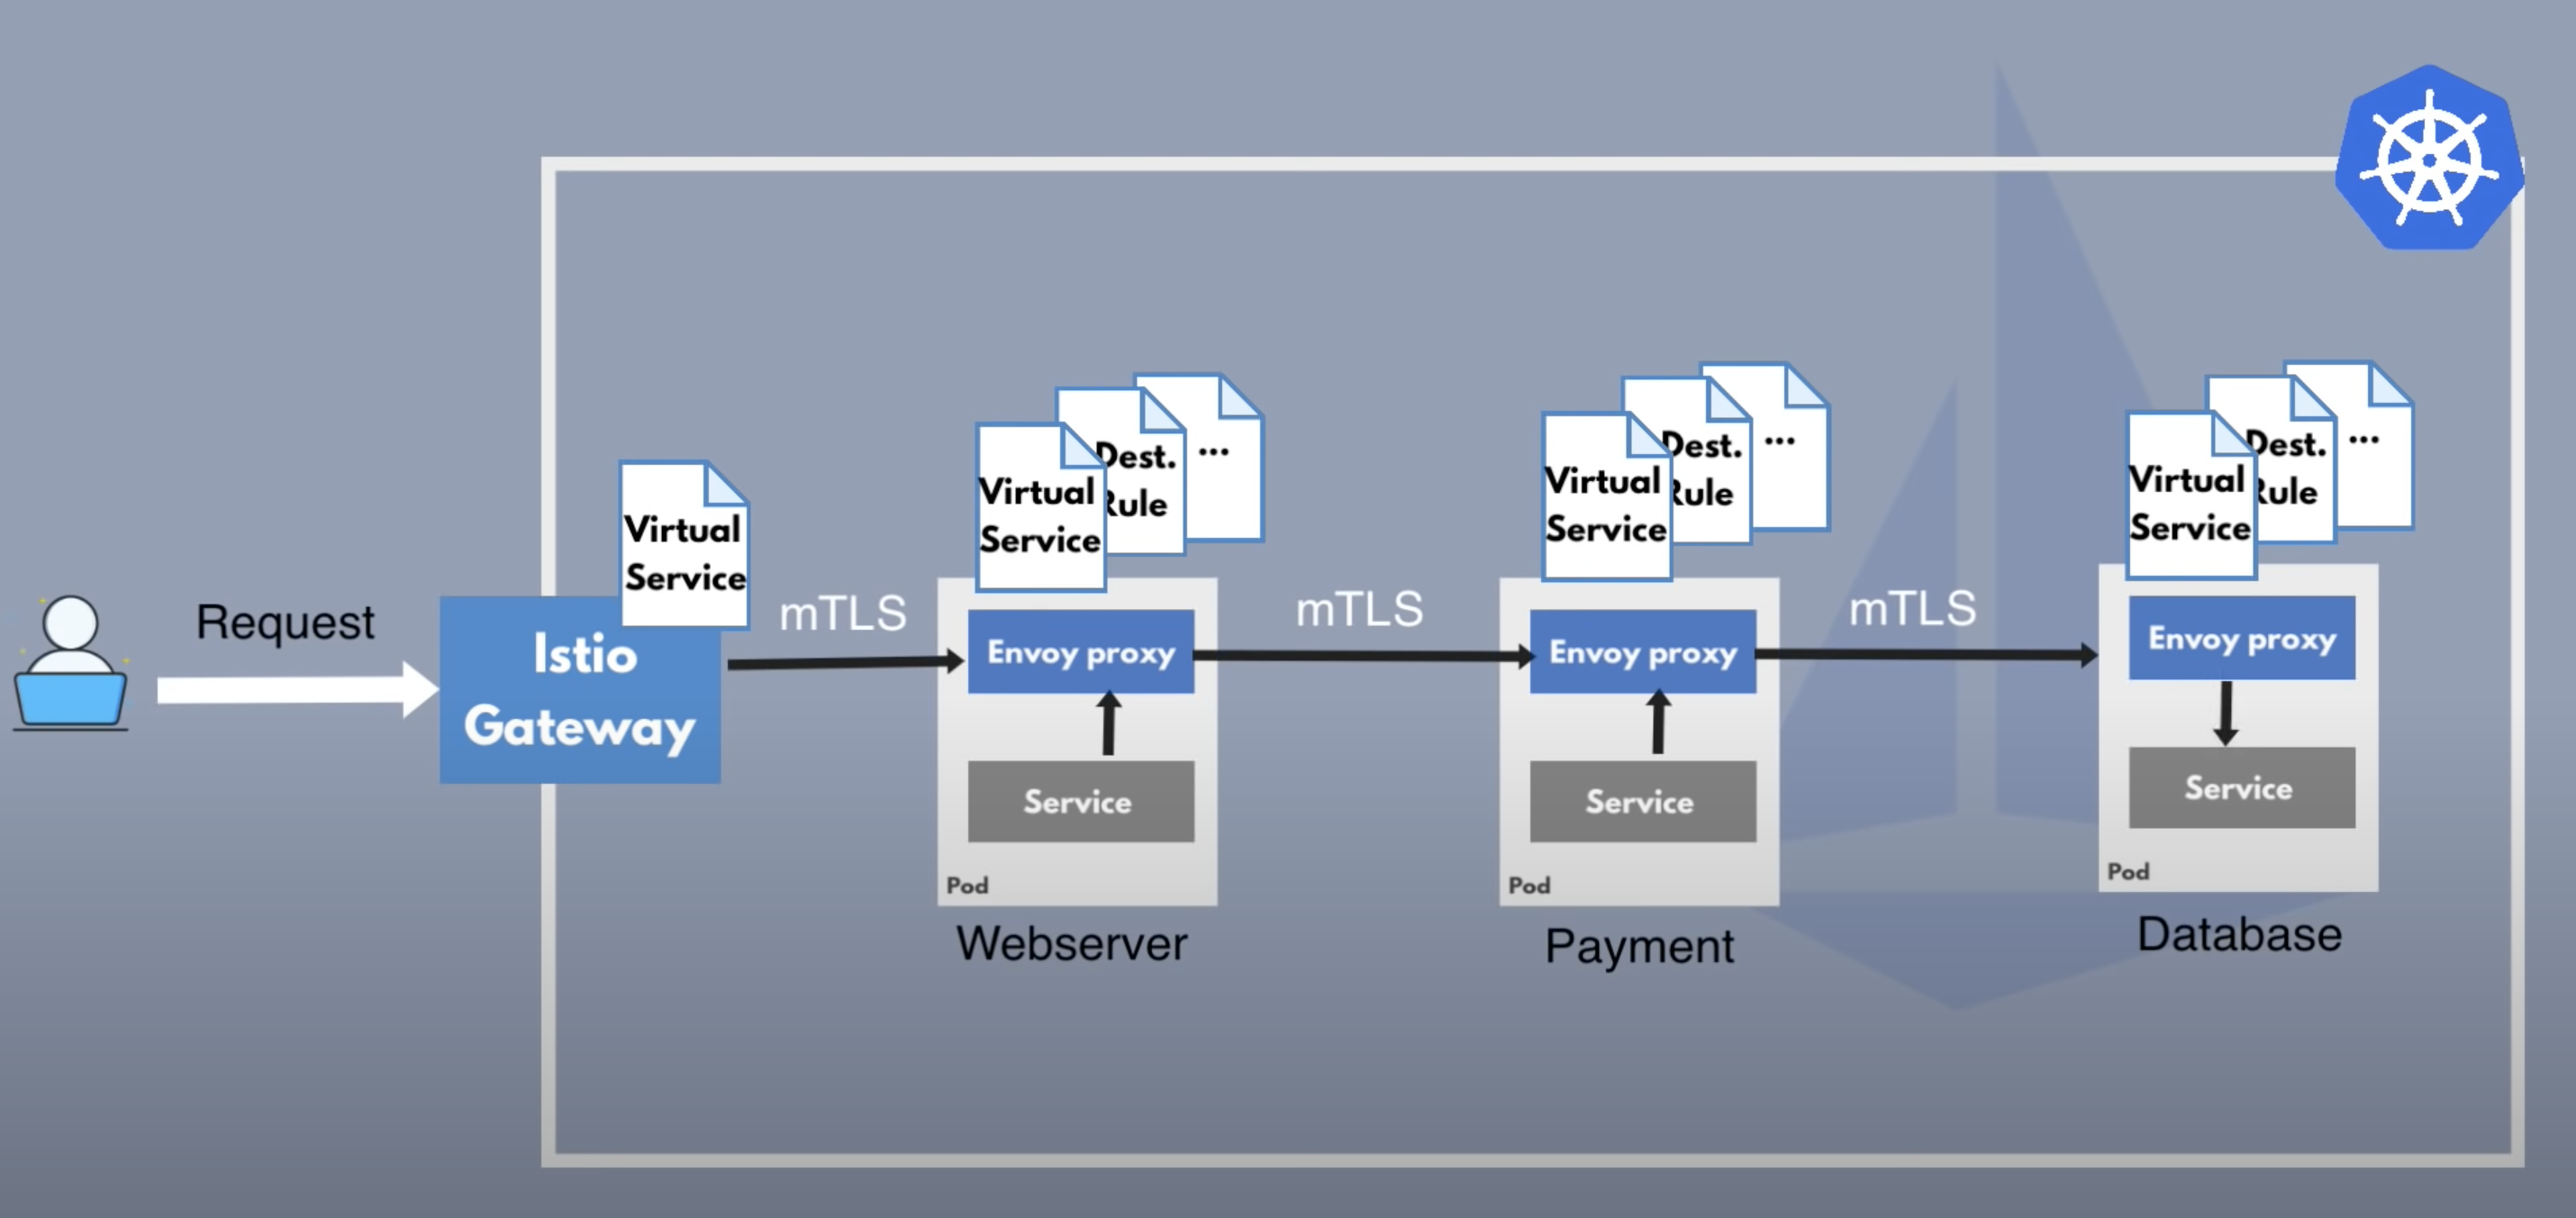
\includegraphics[width=0.7\linewidth]{Pics/2.1.2-p3}
			\caption{Ví dụ về lưu lượng trong Istio}
			\label{fig:2.1.2-3}
		\end{figure}
		
		\subsection{Tổng quan về Envoy Proxy}
		\hspace{0.6cm}Một dịch vụ proxy khi chạy được sắp xếp nằm ngoài quy trình với ứng dụng, ứng dụng sẽ nói chuyện thông qua dịch vụ proxy cứ khi nào nó muốn giao tiếp với các dịch vụ khác. Với Istio, các Envoy proxy được triển khai cùng với tất cả các ứng dụng trong một mạng lưới serves mesh, được quản lý bở services data plane. Vì Envoy là một thành phần quan trọng trong data plane và trong kiến trúc services mesh tổng thể, nên chúng ta cần phải làm quen với nó. Điều này sẽ giúp bạn hiểu rõ hơn về Istio và cách gỡ lỗi hoặc khắc phục sự cố trong quá trình triển khai của bạn.
			\subsubsection{Định nghĩa về Envoy proxy}
		\hspace{0.6cm}Envoy được phát triển bởi Lyft để giải quyết một số vấn đề khó khăn về mạng ứng dụng nảy sinh khi xây dựng các hệ thống phân tán. Nó đã được xây dựng như một dự án nguồn mở vào tháng 9 năm 2016 và một năm sau (tháng 9 năm 2017) nó đã tham gia Nền tảng điện toán  đám mây (CNCF). Envoy được viết bằng C++ với nỗ lực tăng hiệu suất và quan trọng hơn là làm cho nó ổn định hơn và mang tính quyết định hơn ở các mức tải cao hơn.
		
		Envoy là một proxy, vì vậy trước khi đi xa hơn chúng ta nên làm rõ proxy là gì. Proxy là một thành phần mạng trung gian trong kiến trúc mạng được đặt trong giao tiếp giữa máy khách và máy chủ, cho phép nó cung cấp các tính năng bổ sung như các chính sách, bảo mật và quyền riêng tư.
		
		\begin{figure}[h]
			\centering
			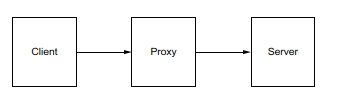
\includegraphics[width=0.7\linewidth]{Pics/2.1.3-p1}
			\caption{Proxy là một trung gian bổ sung các chức năng trong lưu lượng}
			\label{fig:2.1.3-1}
		\end{figure}
		
		Proxy có thể đơn giản hóa những gì máy khách cần biết khi nói chuyện với một dịch vụ. Ví dụ: một dịch vụ có thể được triển khai dưới dạng một tập hợp các phiên bản giống hệt nhau (một cụm), mỗi phiên bản có thể xử lý một lượng tải nhất định. Làm cách nào để máy khách biết phiên bản hoặc địa chỉ IP nào sẽ sử dụng khi đưa ra yêu cầu đối với dịch vụ đó? Một proxy có thể đứng ở giữa với một số nhận dạng hoặc địa chỉ IP duy nhất và máy khách có thể sử dụng nó để giao tiếp với các phiên bản của dịch vụ. Hình 2.7 cho thấy cách proxy xử lý cân bằng tải trên các phiên bản của dịch vụ mà không cần máy khách biết bất kỳ chi tiết nào về cách mọi thứ thực sự được triển khai. Một chức năng phổ biến khác của loại proxy ngược này là kiểm tra tình trạng của các phiên bản trong cụm và định tuyến lưu lượng xung quanh các phiên bản phụ trợ bị lỗi hoặc hoạt động sai. Bằng cách này, proxy có thể bảo vệ máy khách khỏi các thành phần phần phụ trợ đang bị quá tải hoặc lỗi.
		
		\begin{figure}[h]
			\centering
			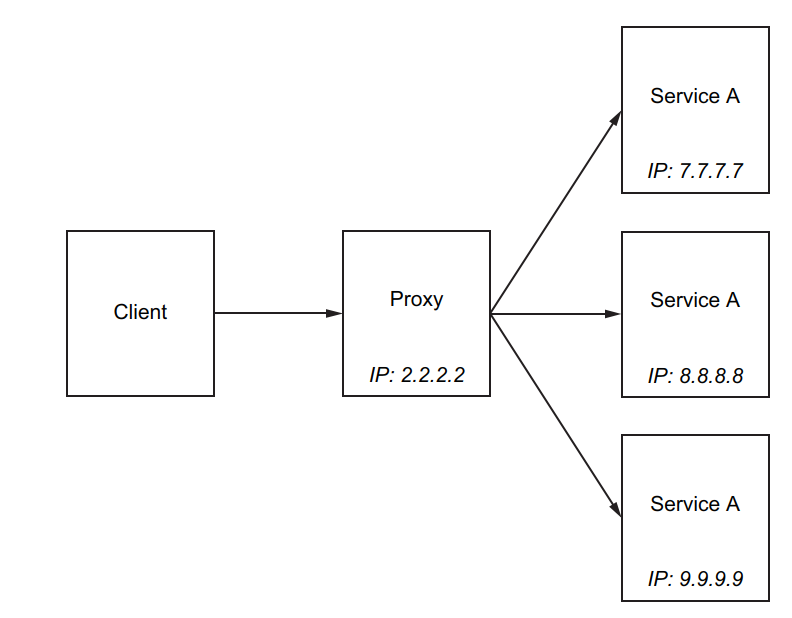
\includegraphics[width=0.7\linewidth]{Pics/2.1.3-p2}
			\caption{Một proxy có thể ẩn cấu trúc liên kết phụ trợ khỏi máy khách và thực hiện các thuật toán để phân phối lưu lượng truy cập một cách công bằng (cân bằng tải).}
			\label{fig:2.1.3-2}
		\end{figure}
		
		Proxy Envoy cụ thể là một proxy tầng ứng dụng mà chúng ta có thể chèn vào đường dẫn của yêu cầu ứng dụng để cung cấp những thứ như tìm kiếm dịch vụ, cân bằng tải và kiểm tra tình trạng, nhưng Envoy có thể làm được nhiều hơn thế. Envoy có thể hiểu các giao thức lớp 7 mà một ứng dụng có thể nói khi giao tiếp với các dịch vụ khác. Ví dụ: Envoy hiểu HTTP 1.1, HTTP 2, gRPC và các giao thức khác và có thể thêm hành vi như request-level timeouts, retries, perretry timeouts, circuit breaking, và các tính năng phục hồi khác. Những thứ như thế này không thể thực hiện được với các proxy cấp kết nối cơ bản (L3/L4) chỉ hiểu các kết nối.
		
		Envoy có thể được mở rộng để hiểu các giao thức ngoài các giao thức mặc định sẵn có. Các bộ lọc đã được viết cho các cơ sở dữ liệu như MongoDB, DynamoDB và thậm chí cả các giao thức không đồng bộ như Giao thức xếp hàng tin nhắn nâng cao (AMQP). Độ tin cậy và mục tiêu minh bạch mạng cho các ứng dụng là những nỗ lực đáng kể, nhưng điều quan trọng không kém là khả năng hiểu nhanh những gì đang xảy ra trong một kiến trúc phân tán, đặc biệt là khi mọi thứ không hoạt động như mong đợi. Vì Envoy hiểu các giao thức cấp ứng dụng và lưu lượng ứng dụng đi qua Envoy, nên proxy có thể thu thập nhiều dữ liệu từ xa về các yêu cầu truyền qua hệ thống, chẳng hạn như thời gian thực hiện các yêu cầu đó, số lượng yêu cầu mà một số dịch vụ nhất định đang xem (thông qua put) và tỷ lệ lỗi mà các dịch vụ đang gặp phải.
		
		\newpage Là một proxy, Envoy được thiết kế để bảo vệ các nhà phát triển khỏi các mối lo ngại về mạng bằng cách chạy các ứng dụng không mang tính quy trình. Điều này có nghĩa là bất kỳ ứng dụng nào được viết bằng bất kỳ ngôn ngữ lập trình nào hoặc với bất kỳ khuôn khổ nào đều có thể tận dụng các tính năng này. Hơn nữa, mặc dù các kiến trúc dịch vụ (SOA, microservice, v.v.) là kiến trúc tất yếu, nhưng Envoy không quan tâm liệu bạn có đang thực hiện các dịch vụ siêu nhỏ hay bạn có các ứng dụng nguyên khối và kế thừa được viết bằng bất kỳ ngôn ngữ nào hay không. Miễn là họ trao đổi bằng các giao thức mà Envoy có thể hiểu (như HTTP), Envoy đều có thể được sử dụng.
		
		Envoy là một proxy rất linh hoạt và có thể được sử dụng trong các vai trò khác nhau: như một proxy ở rìa cụm (như một điểm vào), như một proxy được chia sẻ cho một máy chủ hoặc một nhóm dịch vụ và thậm chí là một proxy cho mỗi dịch vụ như chúng ta thấy với Istio. Với Istio, một proxy Envoy duy nhất được triển khai cho mỗi phiên bản dịch vụ để đạt được sự linh hoạt, hiệu suất và khả năng kiểm soát cao nhất. Chỉ vì ta sử dụng một loại mẫu triển khai (proxy dịch vụ sidecar) không có nghĩa là ta cũng không thể có lợi thế được phân phối với Envoy. Trên thực tế, việc có proxy được triển khai giống nhau ở rìa cũng như được đặt trong lưu lượng ứng dụng có thể giúp cơ sở hạ tầng của ta dễ vận hành và suy luận hơn. Như chúng ta thấy, Envoy có thể được sử dụng ở biên để xâm nhập và liên kết với lưới dịch vụ để cung cấp toàn quyền kiểm soát và quan sát lưu lượng từ điểm nó đi vào cụm cho đến các dịch vụ riêng lẻ trong biểu đồ lời gọi cho một yêu cầu cụ thể.
		
			\subsubsection{Các chức năng chính của Envoy}
		\hspace{0.6cm}Envoy có nhiều tính năng hữu ích cho giao tiếp giữa các dịch vụ. Để giúp hiểu các tính năng và khả năng này, bạn nên nắm rõ các khái niệm Envoy sau đây:
		\begin{itemize}
			\item \textbf{Listeners}—Đưa một cổng ra bên ngoài, nơi mà các ứng dụng có thể kết nối. Ví dụ: một listener trên cổng 80 chấp nhận lưu lượng và áp dụng các hành vi được cấu hình chỉ định cho lưu lượng đó.
			\item \textbf{Route}—Quy tắc định tuyến để xử lý lưu lượng đến từ listener. Ví dụ: nếu một yêu cầu đến và khớp với \textit{/catalog}, hãy hướng lưu lượng truy cập đó đến cụm danh mục \textit{/catalog}.
			\item \textbf{Clusters}—Các dịch vụ cấp trên cụ thể mà Envoy có thể định tuyến lưu lượng. Ví dụ: catalog-v1 và catalog-v2 có thể là các cụm riêng biệt và các tuyến đường có thể chỉ định các quy tắc về cách hướng lưu lượng truy cập đến v1 hoặc v2 của dịch vụ catalog.
		\end{itemize}
		
		Đây là những khái niệm cơ bản về những gì mà Envoy có thể thực hiện đối với lưu lượng L7
		
		Envoy sử dụng thuật ngữ tương tự như thuật ngữ của các proxy khác khi chuyển hướng lưu lượng truy cập. Ví dụ: lưu lượng truy cập đến một listener từ hệ thống cấp dưới. Lưu lượng này được định tuyến đến một trong các cụm của Envoy, cụm này chịu trách nhiệm gửi lưu lượng đó đến một hệ thống cấp trên (như trong hình 2.8). Dòng lưu lượng qua Envoy từ hạ lưu đến thượng nguồn. Bây giờ, hãy chuyển sang một số tính năng của Envoy.
		\begin{figure}[h]
			\centering
			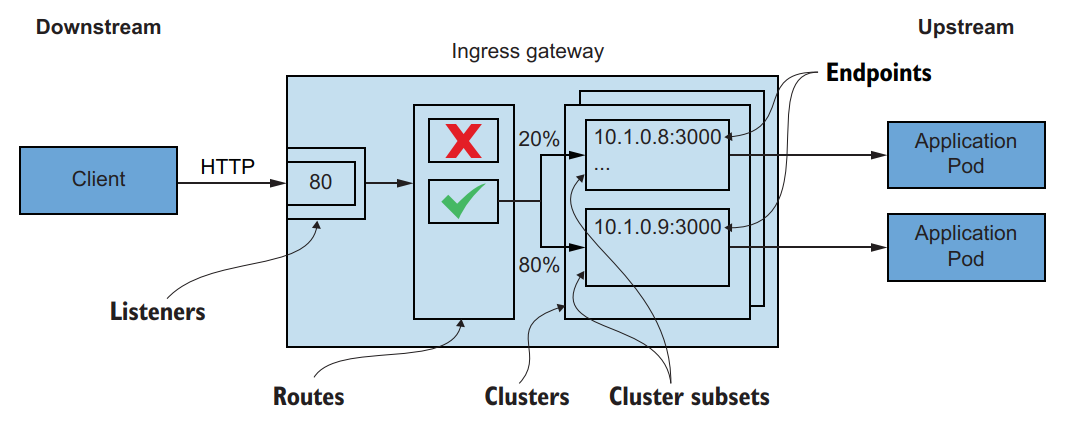
\includegraphics[width=0.9\linewidth]{Pics/2.1.3-p3}
			\caption{Một yêu cầu đến từ một hệ thống cấp dưới thông qua các listeners, đi qua quá trình định tuyến và kết thúc bằng một cụm gửi nó đến một dịch vụ cấp trên.}
			\label{fig:2.1.3-3}
		\end{figure}
	
		\textbf{Service discovery}
		
		Thay vì sử dụng các thư viện runtime đặc thù để tìm kiếm dịch vụ phía máy khách, Envoy có thể tự động thực hiện việc này cho một ứng dụng. Bằng cách định cấu hình Envoy để tìm kiếm các điểm cuối dịch vụ từ một API tìm kiếm đơn giản, các ứng dụng có thể không biết cách tìm thấy các điểm cuối dịch vụ. API tìm kiếm là một API REST đơn giản có thể được sử dụng để bọc các API tìm kiếm dịch vụ phổ biến khác (như HashiCorp Consul, Apache ZooKeeper, Netflix Eureka, v.v.). Control plane của Istio triển khai API này ngay lập tức.
		
		Envoy được xây dựng đặc biệt để dựa vào các bản cập nhật nhất quán cuối cùng cho danh mục tìm kiếm dịch vụ. Điều này có nghĩa là trong một hệ thống phân tán, ta không thể biết chính xác trạng thái của tất cả các dịch vụ mà chúng ta có thể liên lạc và liệu chúng có khả dụng hay không. Điều tốt nhất chúng ta có thể làm là sử dụng kiến thức có sẵn, sử dụng kiểm tra chủ động và thụ động.
		
		Istio đơn giản hoá rất nhiều chi tiết này bằng cách cung cấp một bộ tài nguyên cấp cao hơn giúp điều khiển cấu hình cơ chế tìm kiếm dịch vụ của Envoy. Chúng ta sẽ xem xét kỹ hơn vấn đề này trong suốt cuốn sách.
		
		\textbf{Cân bằng tải}\\
		\hspace{0.6cm}Envoy thực hiện một vài thuật toán cân bằng tải nâng cao mà các ứng dụng có thể tận dụng. Một trong những khả năng thú vị hơn của các thuật toán cân bằng tải của Envoy là cân bằng tải nhận biết cục bộ. Trong tình huống này, Envoy đủ thông minh để ngăn lưu lượng truy cập vượt qua bất kỳ ranh giới nào trừ khi nó đáp ứng các tiêu chí nhất định và sẽ mang lại sự cân bằng lưu lượng tốt hơn. Ví dụ: Envoy đảm bảo rằng lưu lượng dịch vụ đến dịch vụ được định tuyến đến các phiên bản trong cùng một địa điểm trừ khi làm như vậy sẽ tạo ra tình huống lỗi. Envoy cung cấp các thuật toán cân bằng tải vượt trội cho các chiến lược sau:
		\begin{itemize}
			\item 		Random
			\item 		Round robin
			\item 		Weighted, least request
			\item 		Consistent hashing (sticky) 
		\end{itemize}		
		
		\textbf{Kiểm soát và định hướng đường lưu lượng}\\
		Vì Envoy có thể hiểu các giao thức ứng dụng như HTTP 1.1 và HTTP 2 nên nó có thể sử dụng các quy tắc định tuyến tinh vi để hướng lưu lượng truy cập đến các cụm phụ trợ cụ thể. Envoy có thể thực hiện định tuyến proxy ngược cơ bản như ánh xạ máy chủ ảo và định tuyến theo ngữ cảnh; nó cũng có thể thực hiện định tuyến dựa trên tiêu đề và mức độ ưu tiên, retries and timeouts để định tuyến cũng như fault injection.
		
		\textbf{Dịch chuyển và tạo bóng lưu lượng}\\
		Envoy hỗ trợ phân tách/chuyển dịch lưu lượng dựa trên tỷ lệ phần trăm (nghĩa là có trọng số). Điều này cho phép các nhóm nhanh chóng sử dụng các kỹ thuật phân phối liên tục để giảm thiểu rủi ro, chẳng hạn như phát hành canary. Mặc dù chúng giảm thiểu rủi ro cho nhóm người dùng nhỏ hơn, các bản phát hành canary vẫn xử lý lưu lượng người dùng trực tiếp.
		
		Envoy cũng có thể tạo các bản sao của lưu lượng truy cập và tạo bóng cho lưu lượng truy cập đó trong chế độ chạy và quên thành một cụm Envoy. Bạn có thể coi khả năng tạo bóng này giống như phân tách lưu lượng, nhưng các yêu cầu mà cụm cấp trên nhìn thấy là một bản sao của lưu lượng trực tiếp; do đó, chúng ta có thể định tuyến lưu lượng truy cập ẩn đến phiên bản mới của dịch vụ mà không thực sự tác động đến lưu lượng truy cập sản xuất trực tiếp. Đây là một khả năng rất mạnh mẽ để thử nghiệm các thay đổi dịch vụ với lưu lượng khác mà không ảnh hưởng đến khách hàng.
		
		\textbf{Khả năng phục hồi mạng}\\
		Envoy có thể được sử dụng để giảm tải một số loại vấn đề về khả năng phục hồi, nhưng lưu ý rằng trách nhiệm của ứng dụng là tinh chỉnh và định cấu hình các tham số này. Envoy có thể tự động thực hiện hết thời gian chờ yêu cầu cũng như thử lại ở cấp độ yêu cầu (với thời gian chờ cho mỗi lần thử lại). Loại hành vi thử lại này rất hữu ích khi một yêu cầu gặp phải tình trạng mạng không ổn định liên tục. Mặt khác, thử lại khuếch đại có thể dẫn đến lỗi xếp tầng; Envoy cho phép bạn giới hạn hành vi thử lại. Cũng lưu ý rằng vẫn có thể cần thử lại ở cấp độ ứng dụng và không thể giảm tải hoàn toàn cho Envoy. Ngoài ra, khi Envoy gọi các cụm ngược dòng, nó có thể được định cấu hình với các đặc điểm phân vùng như giới hạn số lượng kết nối hoặc yêu cầu chưa xử lý trong chuyến bay và nhanh chóng thất bại bất kỳ kết nối nào vượt quá các ngưỡng đó (với một số rung pha trên các ngưỡng đó). Cuối cùng, Envoy có thể thực hiện phát hiện ngoại lệ, hoạt động giống như một bộ ngắt mạch và loại bỏ các điểm cuối khỏi nhóm cân bằng tải khi chúng hoạt động sai.
		
		\textbf{HTTP/2 và GRPC}\\
		HTTP/2 là một cải tiến đáng kể đối với giao thức HTTP, cho phép ghép các yêu cầu qua một kết nối duy nhất, tương tác đẩy máy chủ, tương tác truyền trực tuyến và áp lực ngược yêu cầu. Envoy được xây dựng ngay từ đầu để trở thành proxy HTTP/1.1 và HTTP/2 với khả năng ủy quyền cho từng giao thức cả hạ lưu và ngược dòng. Ví dụ, điều này có nghĩa là Envoy có thể chấp nhận các kết nối HTTP/1.1 và ủy quyền cho HTTP/2 hoặc ngược lại hoặc ủy quyền HTTP/2 đến cho các cụm HTTP/2 cấp trên. gRPC là một giao thức RPC sử dụng Google Protocol Buffers (Protobuf) nằm trên HTTP/2 và cũng được hỗ trợ bởi Envoy. Đây là những tính năng mạnh mẽ (và khó sửa sai khi triển khai) và phân biệt Envoy với các proxy dịch vụ khác.
		
		\textbf{Khả năng giám sát với Metric Collection}\\
		Như chúng ta đã thấy trong thông báo của Envoy từ Lyft vào tháng 9 năm 2016, một trong những mục tiêu của Envoy là giúp mạng trở nên dễ hiểu. Envoy thu thập một tập hợp lớn các số liệu để giúp đạt được mục tiêu này. Nó theo dõi nhiều chiều xung quanh các hệ thống cấp trên gọi nó, chính máy chủ và các cụm cấp dưới mà nó gửi yêu cầu. Số liệu thống kê của Envoy được theo dõi dưới dạng bộ đếm, đồng hồ đo hoặc biểu đồ. Bảng 3.1 liệt kê một số ví dụ về các loại thống kê được theo dõi cho một cụm cấp dưới.
		\begin{figure}[h]
			\centering
			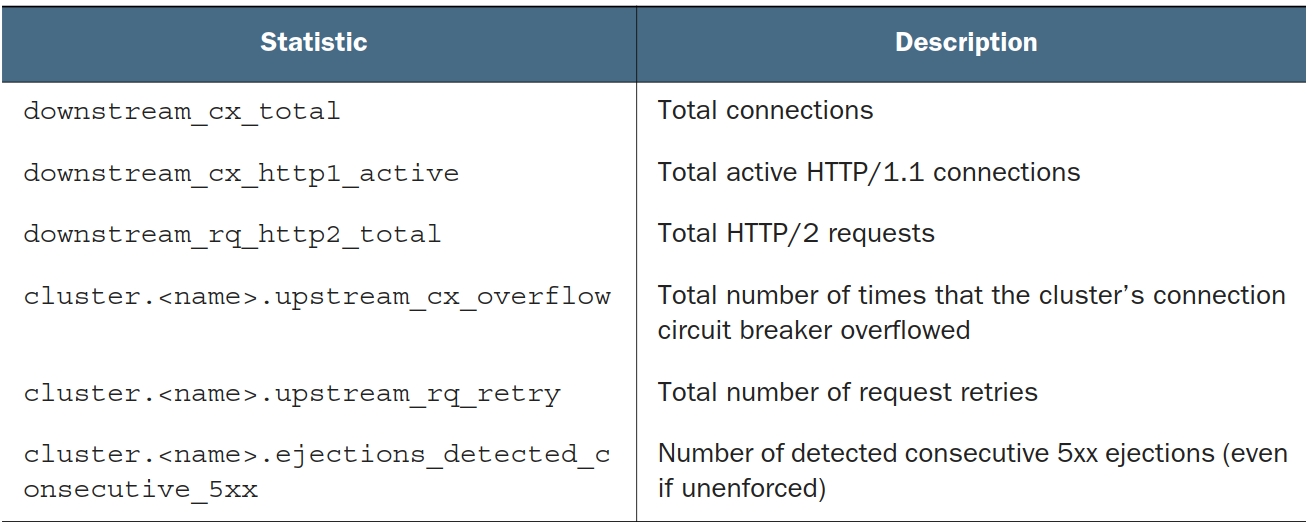
\includegraphics[width=0.7\linewidth]{Pics/2.1.3-p4}
			\caption{Một số số liệu thống kê mà Envoy proxy thu thập}
			\label{fig:2.3.1-4}
		\end{figure}
		
		Envoy có thể phát ra số liệu thống kê bằng cách sử dụng các định dạng và bộ điều hợp có thể định cấu hình. Ngoài ra, Envoy hỗ trợ như sau:
		\begin{itemize}
			\item StatsD
			\item Datadog; DogStatsD
			\item Hystrix formatting
			\item Generic metrics service
		\end{itemize}
		
		\textbf{Khả năng giám sát với Distributed Tracing}\\
		Envoy có thể báo cáo các khoảng thời gian theo dõi cho các công cụ OpenTracing (http://opentracing.io) để trực quan hóa luồng lưu lượng, bước nhảy và độ trễ trong biểu đồ lời gọi. Điều này có nghĩa là bạn không phải cài đặt các thư viện OpenTracing đặc biệt. Mặt khác, ứng dụng chịu trách nhiệm truyền tải các tiêu đề Zipkin cần thiết, điều này có thể được thực hiện với các thư viện trình bao bọc mỏng.
		
		Envoy tạo tiêu đề x-request-id để tương quan các lệnh gọi giữa các dịch vụ và cũng có thể tạo tiêu đề x-b3* ban đầu khi kích hoạt theo dõi. Các tiêu đề mà ứng dụng chịu trách nhiệm tuyên truyền như sau:
		\begin{itemize}
			\item x-b3-traceid
			\item x-b3-parentspanid
			\item x-b3-sampled
			\item x-b3-flags
		\end{itemize}
		
		\textbf{Sử dùng tự động TSL}\\
		Envoy có thể dừng lưu lượng Transport Level Security (TLS) dành cho một dịch vụ cụ thể ở cả rìa của cụm và sâu bên trong mạng lưới proxy dịch vụ. Một khả năng thú vị hơn là Envoy có thể được sử dụng để tạo lưu lượng truy cập TLS đến cụm cấp trên thay mặt cho ứng dụng. Đối với các nhà phát triển và nhà điều hành doanh nghiệp, điều này có nghĩa là ta không phải loay hoay với các cài đặt dành riêng cho ngôn ngữ và keystores hay truststores. Bằng cách có Envoy trong đường dẫn yêu cầu, chúng ta có thể tự động nhận TLS và thậm chí cả TLS lẫn nhau.
		
		\textbf{Rate Limit}\\
		Một khía cạnh quan trọng của khả năng phục hồi là khả năng hạn chế hoặc giới hạn quyền truy cập vào các tài nguyên được bảo vệ. Các tài nguyên như cơ sở dữ liệu hoặc bộ đệm hoặc dịch vụ dùng chung có thể được bảo vệ vì nhiều lý do:
		\begin{itemize}
			\item Expensive to call (per-invocation cost)
			\item Slow or unpredictable latency
			\item Fairness algorithms needed to protect against starvation
		\end{itemize}
		
		Đặc biệt là khi các dịch vụ được định cấu hình để thử lại, chúng ta không muốn phóng đại tác động của một số lỗi nhất định trong hệ thống. Để giúp điều tiết các yêu cầu trong các tình huống này, chúng ta có thể sử dụng dịch vụ giới hạn tốc độ toàn bộ. Envoy có thể tích hợp với dịch vụ giới hạn tốc độ ở cả cấp độ mạng (trên mỗi kết nối) và HTTP (theo yêu cầu).
		
		\textbf{Envoy mở rộng}\\
		Về cốt lõi, Envoy là một công cụ xử lý byte trên đó có thể xây dựng các codec giao thức (lớp 7) (được gọi là bộ lọc). Envoy làm cho việc xây dựng các bộ lọc bổ sung trở thành trường hợp sử dụng cụ thể và là một cách thú vị để mở rộng Envoy cho các trường hợp sử dụng cụ thể. Bộ lọc Envoy được viết bằng C++ và được biên dịch thành mã nhị phân Envoy. Ngoài ra, Envoy hỗ trợ tập lệnh Lua(www.lua.org) và WebAssugging (Wasm) để có cách tiếp cận ít xâm lấn hơn nhằm mở rộng chức năng của Envoy.
		
		\textbf{So sánh với các loại proxy khác}\\
		Điểm hấp dẫn của Envoy là nó đóng vai trò của proxy ứng dụng hoặc dịch vụ, trong đó Envoy tạo điều kiện cho các ứng dụng nói chuyện với nhau thông qua proxy và giải quyết các vấn đề về độ tin cậy và khả năng giám sát. Các proxy khác đã phát triển từ bộ cân bằng tải và máy chủ web thành các proxy có khả năng và hiệu suất cao hơn. Một số cộng đồng này không phát triển như vậy hoặc là mã nguồn nguồn đóng và đã mất một thời gian để phát triển đến mức chúng có thể được sử dụng trong các tình huống từ ứng dụng đến ứng dụng. Đặc biệt, Envoy tỏa sáng so với các proxy khác trong các lĩnh vực như sau:
		\begin{itemize}
			\item Extensibility with WebAssembly
			\item Open community
			\item Modular codebase built for maintenance and extension
			\item HTTP/2 support (upstream and downstream)
			\item Deep protocol metrics collection
			\item C++ / non-garbage-collected
			\item Dynamic configuration, no need for hot restarts
		\end{itemize}
	
		\textbf{Cấu hình Envoy}\\
		
		Envoy được điều khiển bởi một tệp cấu hình ở định dạng JSON hoặc YAML. Tệp cấu hình chỉ định listener, route và cluster cũng như các cài đặt dành riêng cho máy chủ như có bật API quản trị hay không, vị trí nhật ký truy cập, theo dõi cấu hình công cụ, v.v. Nếu bạn đã quen thuộc với Envoy hoặc cấu hình Envoy, bạn có thể biết rằng có nhiều phiên bản khác nhau của cấu hình Envoy. Các phiên bản ban đầu, v1 và v2, không được dùng nữa để chuyển sang phiên bản v3. Chúng tôi chỉ xem xét cấu hình v3 trong cuốn sách này, vì đó là phiên bản tiếp theo và là những gì Istio sử dụng.
		
		API cấu hình v3 của Envoy được xây dựng trên gRPC. Envoy và những người triển khai API v3 có thể tận dụng các khả năng phát trực tuyến khi gọi API và giảm thời gian cần thiết để các proxy của Envoy hội tụ về cấu hình chính xác. Trên thực tế, điều này giúp loại bỏ nhu cầu thăm dò API và cho phép máy chủ đẩy các bản cập nhật lên Envoys thay vì thăm dò proxy theo các khoảng thời gian định kỳ.
	\section{Quản lý mạng giữa các Microservices với Istio}
		\subsection{Tổng quan về Istio Ingress Gateway}
		\hspace{0.6cm}Istio có một gateway vào đóng vai trò là điểm vào mạng và chịu trách nhiệm bảo vệ và kiểm soát quyền truy cập vào cụm bởi lưu lượng truy cập bắt nguồn từ bên ngoài cụm. Ngoài ra, gateway của Istio xử lý cân bằng tải và định tuyến máy chủ ảo.
		
		Hình 2.10 cho thấy thành phần cổng vào của Istio cho phép lưu lượng truy cập vào cụm và thực hiện chức năng proxy ngược. Istio sử dụng một proxy Envoy duy nhất làm gateway. Chúng ta đã thấy ở trên rằng Envoy là một proxy có khả năng kết nối dịch vụ đến dịch vụ, nhưng nó cũng có thể được sử dụng để cân bằng tải và định tuyến lưu lượng từ bên ngoài lưới dịch vụ đến các dịch vụ chạy bên trong nó. Tất cả các tính năng của Envoy mà chúng ta đã thảo luận trong chương trước cũng có sẵn ở đây.
		
		Chúng ta hãy xem xét kỹ hơn cách Istio sử dụng Envoy để triển khai thành phần gateway của nó. Khi cài đặt Istio, hình 2.11 hiển thị danh sách các thành phần tạo nên control plane và các thành phần bổ sung hỗ trợ cho nó.
		
		Trong hình 2.11, bên cạnh Pod istio-ingressgateway, hãy lưu ý thành phần istio-egressgateway. Thành phần này chịu trách nhiệm định tuyến lưu lượng ra khỏi cụm. Cổng ra được cấu hình với cùng tài nguyên như cổng vào mà chúng ta sẽ thấy trong chương này.
		
		\begin{figure}[h!]
			\centering
			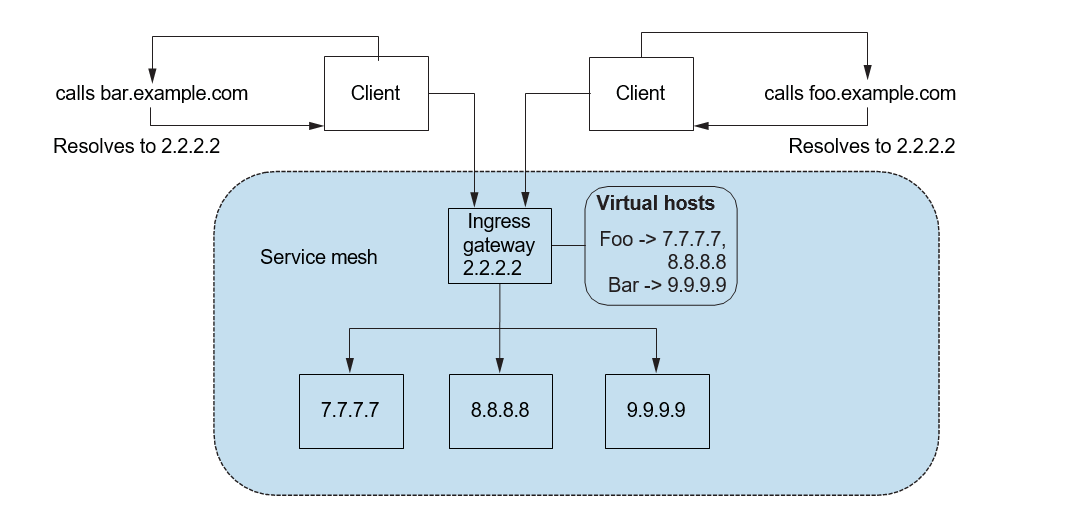
\includegraphics[width=0.6\linewidth]{Pics/2.2.1-p1}
			\caption{Istio Gateway đóng vai trò là điểm vào mạng và sử dụng proxy Envoy để thực hiện định tuyến và cân bằng tải.}
			\label{fig:2.2.1-1}
		\end{figure}
		
		\begin{figure}[h!]
			\centering
			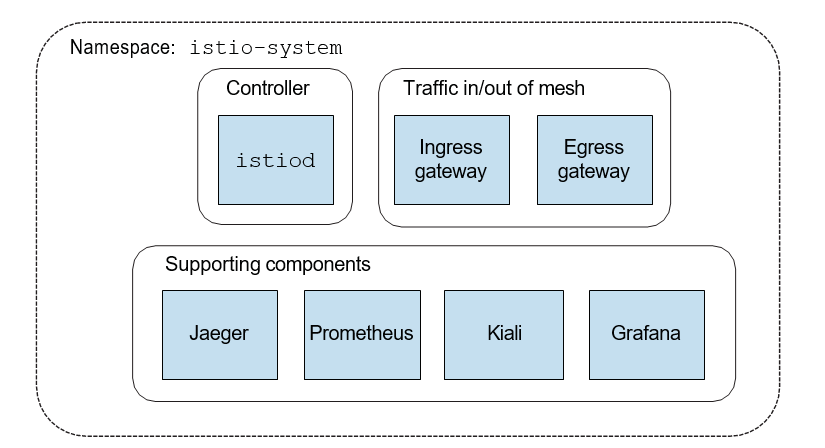
\includegraphics[width=0.7\linewidth]{Pics/2.2.1-p2}
			\caption{Cấu trúc một control plane và các thành phần phụ trợ}
			\label{fig:2.2.1-2}
		\end{figure}
		
		\subsection{Định tuyến đường đi các Microservices trong Kubernetes sử dụng Istio}
			\hspace{0.6cm} Trong kiến trúc monolith, chúng ta có một dịch vụ khổng lồ duy nhất với tất cả logic nghiệp vụ để xử lý tất cả các yêu cầu từ người dùng, nhưng trong kiến trúc microservices, chúng ta có nhiều dịch vụ tập trung vào logic nghiệp vụ cụ thể. Một yêu cầu của người dùng duy nhất có thể trờ thành nhiều yêu cầu cho các dịch vụ phụ thuộc.
			
			\begin{figure}[h!]
				\centering
				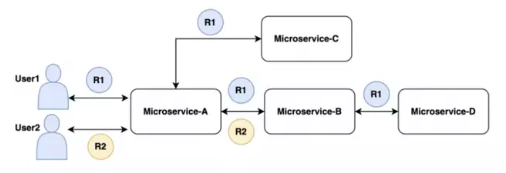
\includegraphics[width=0.9\linewidth]{Pics/2.2.2-p4}
				\caption{Ví dụ về mô hình microservices}
				\label{fig:2}
			\end{figure}
		
			Như thể hiện trong sơ đồ trên, một yêu cầu của người dùng tới microservice-A được gửi đến microservice-B, microservice-C, và microservice-D. Cuối cùng, một phản hồi được gửi đến người dùng. Bây giờ, giả sử microservice-B có một tính năng mới, cần được phát triển và thử nghiệm trên một nhóm user được chọn cụ thể ở đây là User1, hoặc cho tỉ lệ 10\% người dùng có thể dụng tính năng mới này. 
			Để giải quyết bài toán trên Istio đã cung cấp một số cơ chế định tuyến sau:
			\begin{itemize}
				\item Canary deployment: Một trong những lợi ích của dự án Istio là nó cung cấp khả năng kiểm soát cần thiết để triển khai các dịch vụ canary. Ý tưởng đằng sau việc triển khai canary là giới thiệu một phiên bản mới của dịch vụ bằng cách thử nghiệm phiên bản đó mới bằng cách sử dụng một tỷ lệ nhỏ lưu lượng truy cập của người dùng và sau đó nếu dịch vụ không có lỗi phát sinh, có thể tăng tỷ lệ phần trăm lên, có thể dần dần trong khi đồng thời loại bỏ dần phiên bản cũ. Nếu xảy ra sự cố trong quá trình thực hiện, có thể cho tất cả lưu lượng truy cập của người dùng trở về phiên bản cũ.
				\item Dark release: Khi nói đến việc triển khai phần mềm, bất cứ điều gì có thể làm để giảm thiểu rủi ro đều đáng được cân nhắc. Chạy song song nhiều phiên bản của một dịch là một cách rất hiệu quả và đã được chứng minh để kiểm tra phiên bản tiếp theo của bạn, đồng thời Istio cho phép bạn sử dụng các dịch vụ bí mật — một phiên bản chưa từng thấy của vi dịch vụ của bạn — mà không bị ảnh hưởng đến sản phẩm. Đó là tính năng dark release, tính năng này cho phép chỉ cố giới hạn một số người như các kĩ sư hoặc kiểm thử phần mềm có thể truy cập vào chức năng này.
				\item Traffic mirroring: giả sử chúng ta muốn đánh giá hiệu suất của dịch vụ mới của chúng ta mới tạo ra mà không muốn khách hàng vào được dịch vụ mới này chúng ta có thể sử dụng tính năng này để tất các lưu lượng truy cập đang đi vào phiên bản hiện tại và sao chép các lưu lượng đó và đưa lưu lượng truy cập đó vào dịch vụ mới chúng ta muốn kiểm thử.
			\end{itemize}
			
			
		\subsection{Giải quyết các vấn đề về mạng trong Microservices}
\hspace{0.6cm}Khi chúng ta có lưu lượng truy cập vào cụm của mình thông qua Istio gateway, chúng ta có thể điều khiển lưu lượng truy cập ở cấp độ yêu cầu và kiểm soát chính xác nơi định tuyến các yêu cầu. Trong chương trước, chúng ta đã đề cập đến kiểm soát lưu lượng cho định tuyến có trọng số, định tuyến dựa trên kết hợp yêu cầu và một số kiểu mẫu phát hành nhất định mà sau đó có thể được kích hoạt. Chúng ta cũng có thể sử dụng khả năng điều khiển lưu lượng này để định tuyến né tránh các sự cố trong trường hợp xảy ra lỗi ứng dụng, phân vùng mạng và các sự cố lớn khác.

Vấn đề với các hệ thống phân tán là chúng thường bị lỗi theo những cách không thể lường trước và chúng ta không thể thực hiện các hành động thay đổi lưu lượng theo cách thủ công. Chúng ta cần một cách để xây dựng các hành động hợp lý tác động vào ứng dụng để chúng có thể tự phản hồi khi gặp sự cố. Chúng ta có thể làm điều đó với Istio, bao gồm thêm timeouts, retries, and circuit breaking mà không phải thay đổi mã nguồn ứng dụng. Trong chương này, chúng ta xem xét cách thực hiện điều này và những tác động đối với phần còn lại của hệ thống.
			\subsubsection{Xây dựng khả năng phục hồi cho ứng dụng}
\hspace{0.6cm}Microservices phải được xây dựng với khả năng phục hồi là mối quan tâm hàng đầu. Thế giới nơi mà mọi thứ “just build it so it won’t fail” là không có thật; và khi xảy ra sự cố, chúng ta có nguy cơ bị mất truy cập tất cả các dịch vụ của mình. Khi chúng ta xây dựng các hệ thống phân tán với các dịch vụ giao tiếp qua mạng, chúng ta có nguy cơ tạo ra nhiều điểm lỗi hơn và đối mặt với khả năng xảy ra lỗi nghiêm trọng. Chủ sở hữu dịch vụ nên áp dụng một vài chức năng khôi phục nhất quán trên các ứng dụng và dịch vụ của họ.

Nếu dịch vụ A gọi dịch vụ B, như được mô tả trong hình 2.18 và gặp phải độ trễ trong các yêu cầu được gửi đến các điểm đầu cuối cụ thể của dịch vụ B, thì chúng ta muốn dịch vụ đó chủ động xác định điều này và định tuyến đến các điểm đầu cuối khác, các nơi khả dụng khác hoặc thậm chí các khu vực khác. Nếu dịch vụ B gặp lỗi không liên tục, chúng ta có thể gửi lại một yêu cầu không thành công. Tương tự, nếu chúng ta gặp sự cố khi gọi dịch vụ B, chúng ta có thể tạm dừng lại cho đến khi dịch vụ này có thể khôi phục sau bất kỳ sự cố nào mà nó có thể gặp phải. Nếu chúng tôi tiếp tục sử dụng dịch vụ B (và trong một số trường hợp, tăng tải khi chúng ta gửi lại các yêu cầu), thì chúng ta có nguy cơ làm quá tải dịch vụ. Tình trạng quá tải này có thể ảnh hưởng đến dịch vụ A và bất kỳ điều gì phụ thuộc vào các dịch vụ này và gây ra các lỗi chồng lỗi đáng kể.
\begin{figure}[h]
	\centering
	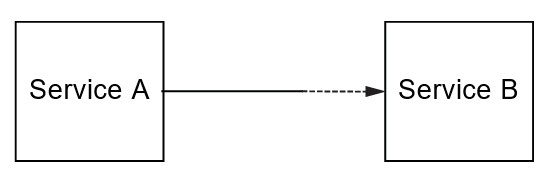
\includegraphics[width=0.7\linewidth]{Pics/2.2.3-p1}
	\caption{Dịch vụ A, dịch vụ gọi B, có thể đang gặp sự cố.}
	\label{fig:2.2.3-1}
\end{figure}

Giải pháp là xây dựng các ứng dụng của chúng tôi để dự kiến các lỗi và có cách để chúng tự động cố gắng khắc phục hoặc quay lại các đường dẫn thay thế khi phục vụ một yêu cầu. Ví dụ: khi dịch vụ A gọi dịch vụ B và bắt đầu gặp sự cố, chúng ta có thể thử gửi lại một yêu cầu, giới hạn thời gian của các yêu cầu hoặc hủy bất kỳ yêu cầu gửi đi nào khác bằng cách sử dụng circuit-breaking. Istio có thể được sử dụng để giải quyết các vấn đề này một cách dễ dàng để các ứng dụng có cách triển khai chính xác và nhất quán cho các vấn đề về khả năng phục hồi bất kể ứng dụng được viết bằng ngôn ngữ lập trình nào.

			\subsubsection{Cân bằng tải phía máy khách}
\hspace{0.6cm}Cân bằng tải phía máy khách là hoạt động thông báo cho khách hàng về các điểm đầu cuối khác nhau có sẵn cho một dịch vụ và cho phép khách hàng chọn các thuật toán cân bằng tải cụ thể để phân phối yêu cầu tốt nhất trên các điểm đầu cuối. Điều này làm giảm nhu cầu dựa vào cân bằng tải tập trung, vốn có thể tạo ra các nút cổ chai và điểm gây lỗi, đồng thời cho phép khách hàng thực hiện các yêu cầu trực tiếp đến các điểm đầu cuối cụ thể mà không cần phải thực hiện thêm các bước không cần thiết. Do đó, khách hàng và dịch vụ của chúng ta có thể mở rộng quy mô tốt hơn và đối phó với cấu trúc liên kết đang thay đổi hằng ngày.

Istio sử dụng khả năng tìm kiếm dịch vụ và điểm đầu cuối để trang bị cho proxy phía máy khách trong giao tiếp giữa dịch vụ với dịch vụ thông tin chính xác và cập nhật nhất, như minh họa trong hình 2.19. Sau đó, nhà phát triển và nhà điều hành dịch vụ có thể cấu hình hành vi cân bằng tải phía máy khách này thông qua cấu hình Istio.
\begin{figure}[h]
	\centering
	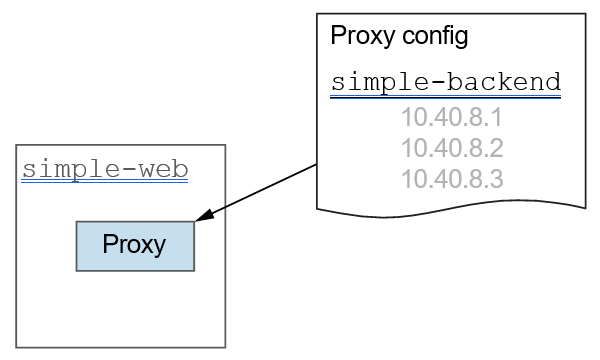
\includegraphics[width=0.7\linewidth]{Pics/2.2.3-p2}
	\caption{Proxy web đơn giản dùng các điểm đầu cuối phụ trợ.}
	\label{fig:2.2.3-2}
\end{figure}

Nhà khai thác và nhà phát triển dịch vụ có thể cấu hình thuật toán cân bằng tải mà máy khách sử dụng bằng cách xác định tài nguyên DestinationRule. Dịch vụ Proxy của Istio dựa trên Envoy và hỗ trợ các thuật toán cân bằng tải của Envoy, một số thuật toán bao gồm:
\begin{itemize}
	\item Round robin (Mặc định)
	\item Random
	\item Weighted least request
\end{itemize}
			\subsubsection{Cân bằng tải nhận biết cục bộ}
\hspace{0.6cm}Một vai trò của control plane như với Istio là nắm được cấu trúc liên kết của dịch vụ và cách cấu trúc liên kết đó có thể phát triển. Một lợi thế của việc nắm được1 cấu trúc liên kết tổng thể của các dịch vụ trong lưới dịch vụ là tự động đưa ra các quyết định định tuyến và cân bằng tải dựa trên kinh nghiệm như vị trí của dịch vụ và dịch vụ ngang hàng.

Istio hỗ trợ một loại cân bằng tải cung cấp trọng số cho các tuyến và đưa ra các quyết định định tuyến dựa trên vị trí của một khối lượng công việc cụ thể. Ví dụ: Istio có thể xác định khu vực và vùng khả dụng trong đó một dịch vụ cụ thể được triển khai và ưu tiên cho các dịch vụ gần hơn. Nếu các dịch vụ phụ trợ được triển khai trên nhiều khu vực (tây Mỹ, đông Mỹ, tây Âu), thì có nhiều tùy chọn để gọi dịch vụ đó. Nếu một dịch vụ web được triển khai ở khu vực phía tây của chúng ta, chúng tôi muốn các cuộc gọi từ dịch vụ web đến dịch vụ phụ trợ để duy trì cục bộ ở phía tây của chúng ta (xem hình 2.20). Nếu chúng ta đối xử bình đẳng với tất cả các điểm đầu cuối, chúng ta có thể sẽ phải chịu độ trễ cao cũng như chi phí khi chúng ta thực hiện chuyển vùng hoặc khu vực.
\begin{figure}[h]
	\centering
	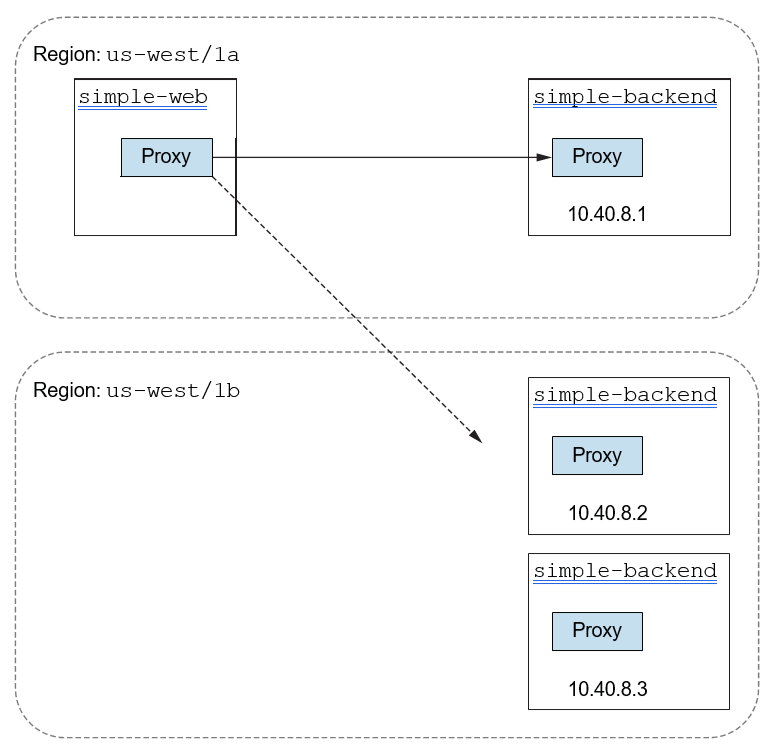
\includegraphics[width=0.7\linewidth]{Pics/2.2.3-p3}
	\caption{Ưu tiên các dịch vụ cục bộ}
	\label{fig:2.2.3-3}
\end{figure}
\newpage
\section{Giám sát các Microservices với Istio}
	{\hspace{0.6cm}Hệ thống giám sát dùng để thu thập thông tin về phần cứng và phần mềm của một hệ thống. Hệ thống giám sát có thể thu thập từ trạng thái của của server (CPU, memory, network, …) cho đến những thông tin chi tiết về cách server xử lý request đến từ người dùng (số lượng requests/s, thời gian server xử lý requests, …), hoặc là cái file nhật kí của hệ thống hoặc ứng dụng.\\
	
	Một hệ thống giám sẽ giúp các quản có một cái nhìn dễ dàng về chất lượng và những vấn đề xảy ra với sản phẩm. Nó sẽ tự động cảnh báo cho chúng ta ngay khi phát hiện ra điều bất thường. Bây giờ, thay vì được người dùng thông báo rằng server gặp trục trặc, chúng ta sẽ sớm phát hiện và giải quyết trước khi người dùng nhận ra. Hơn nữa, đối với các hệ thống đủ lớn và phức tạp, hệ thống giám sát còn giúp chúng ta biết được những thành phần nào hay gặp sự cố để có thể tập trung cải thiện chất lượng.
		\subsection{Cách Istio Giám sát các lưu lượng mạng}
	{\hspace{0.6cm}Istio ở một vị trí đặc biệt để giúp một hệ thống giám sát có thể lấy dữ liệu của Istio proxy là Envoy, và Envoy proxy đứng giữa đường truyền của các service. Thông qua proxy dịch vụ Envoy, Istio có thể nắm bắt các chỉ số quan trọng liên quan đến xử lý yêu cầu và tương tác dịch vụ, chẳng hạn như số lượng request mỗi giây, thời gian thực hiện request, số lượng requests không thành công mà và nhiều thông tin khác.\\		
	
	Istio đi kèm với một số công cụ mẫu sẵn dùng như Prometheus, Grafana và Kiali, có thể giúp các quản trị viên dễ dàng giám sát các microservice một cách tập trung và có thể vẽ các biểu đồ cho các chỉ số của microserivces và làm quản trị viên dễ dàng đánh giá trạng thái của các microservice.
	
	Envoy có thể giữ một tập hợp lớn các số liệu về kết nối, yêu cầu và thời gian chạy mà chúng ta có thể sử dụng để tạo thành một bức tranh về tình trạng mạng và giao tiếp của dịch vụ. Chúng ta có thể sử dụng câu lệnh:
	\begin{lstlisting}
		$ kubectl exec -it deploy/webapp -c istio-proxy \
		-- curl localhost:15000/stats
	\end{lstlisting}
	Và chúng ta có thể thấy rất nhiều các chỉ số mà envoy proxy cung cấp.Đối với lưu lượng HTTP, HTTP/2 và GRPC, Istio tạo các chỉ số sau:
	\begin{itemize}				
		\item istio\_requests\_total: Đây là bộ đếm được tăng lên cho mọi yêu cầu được xử lý bởi proxy Istio.
		\item istio\_request\_duratio\_milliseconds: Là thời gian Istio proxy xử lý một request.
		\item  istio\_request\_bytes: tổng số byte của HTTP request
		\item  istio\_response\_bytes: tổng số byte của HTTP response
		\item  istio\_request\_messages\_total: Đây là bộ đếm tăng dần cho mỗi tin nhắn gRPC được gửi từ máy khách.
		\item istio\_response\_messages\_total: Đây là bộ đếm tăng dần cho mỗi tin nhắn gRPC được gửi từ server.
	\end{itemize}
	Đối với lưu lượng TCP, Istio tạo các chỉ số sau:
	\begin{itemize}				
		\item istio\_tcp\_sent\_bytes\_total: Đây là bộ đếm đo kích thước của tổng số byte được gửi trong quá trình phản hồi trong trường hợp kết nối TCP.
		\item istio\_tcp\_received\_bytes\_total: Đây là bộ đếm đo kích thước của tổng số byte nhận được trong khi yêu cầu trong trường hợp kết nối TCP.
		\item istio\_tcp\_connections\_opened\_total: Đây là bộ đếm được tăng lên cho mỗi kết nối được mở.
		\item istio\_tcp\_connections\_closed\_total: Đây là bộ đếm được tăng lên cho mọi kết nối đã đóng.
	\end{itemize}
	Từ các chỉ số được Envoy cung cấp các hệ thống giám sát như promethues có thể lấy các chỉ số này về và Grafana sẽ cung lấy các chỉ số này từ promethues và vẽ ra các biểu đồ cho quản trị viên có thể quan sát các 
	
	\begin{figure}[h]
		\centering
		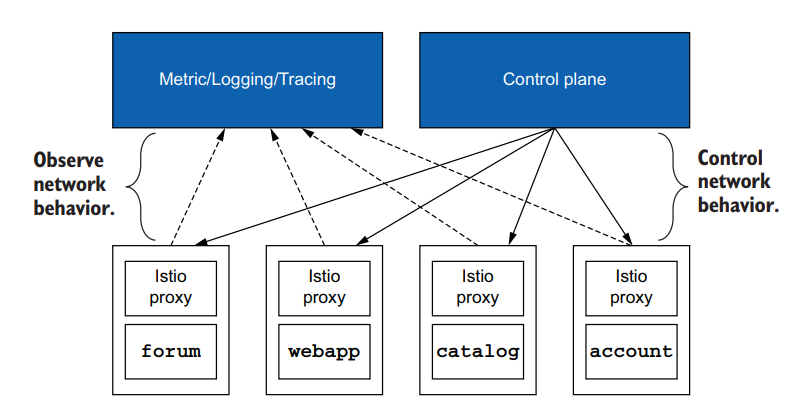
\includegraphics[width=0.5\linewidth]{Pics/2.3.1-p1}
		\caption{Mô hình proxy kết hợp với các hệ thống quản lý}
		\label{fig:2}
	
\end{figure}
	\subsection{Theo dõi phân tán với Istio}
		{\hspace{0.6cm}Khi xây dựng một ứng dụng theo kiến trúc microservice, chúng ta tạo ra một mạng lưới phân tán của các microserivce để chúng hoạt động như một ứng dụng bình thường, như được minh họa hình 2.3.2. Khi có sự cố bắt đầu xảy ra khi các mircrosevice gọi nhau, điều quan trọng là phải hiểu điều gì đang xảy ra để có thể chẩn đoán và khắc phục nhanh chóng. Trong các phần trước, chúng ta đã thấy cách Istio có thể giúp thu thập các số liệu và phép đo từ xa liên quan đến kết nối mạng thay mặt cho ứng dụng. Theo dõi phân tán giúp các quản trị viên có thể chẩn đoán microservice nào đang bị lỗi.}\\
			
		\begin{figure}[h]
			\centering
			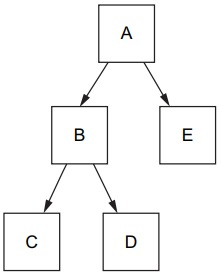
\includegraphics[width=0.3\linewidth]{Pics/Untitled}
			\caption{Mô hình để thực hiện một request cần đi qua nhiều microservice.}
			\label{fig:untitled}
		\end{figure}
	
		Khi có request bị lỗi khi đi qua nhiều các microservice, quản trị viên phải hiểu chuyện gì đang xảy ra và chuẩn đoán lỗi để có thể nhanh chóng khắc phục. Trong phần trước, Istio đã thu thập các chỉ số về mạng cho các microserivce. Ở phần này, Istio hỗ trợ việc theo dõi phân phân tán để chuẩn đoán khi các request bị lỗi khi đi qua các microservice và tìm xem request bị lỗi ở microservice nào.\\
		
		Theo dõi phân tán cung cấp thông tin chi tiết về các thành phần của hệ thống phân khi phục vụ các request. Nó được giới thiệu bởi bài báo Google Dapper (“Dapper, a LargeScale Distributed Systems Tracing Infrastructure” 2010, https://research.google/pubs/pub36356) 
		và nói về việc đánh nhãn các các request bằng các ID tương ứng với mỗi request đại diện cho các cuộc gọi từ dịch vụ đến dịch vụ và ID theo dõi đại diện cho một request cụ thể khi các service gọi lẫn nhau. Istio proxy có thể thêm các metadata khi các request đi qua chúng.\\
		
		OpenTelemetry là một framework bao gồm OpenTracing, OpenTracing là một API không phụ thuộc vào nhà cung cấp để giúp các kĩ sư phần mềm dễ dàng đưa công cụ theo dõi vào mã nguồn của họ. Theo dõi phân tán, một phần, dựa vào các kĩ sư phần mềm viết code của họ và đánh nhãn các request khi chúng được ứng dụng xử lý và đưa ra các request mới cho các hệ thống khác. Công cụ theo dõi giúp tổng hợp bức tranh toàn thể về luồng request, có thể được sử dụng để xác định các nguồn bị lỗi trong kiến trúc microservice của ứng dụng.\\
		
		Ở dạng đơn giản nhất, theo dõi phân tán với OpenTracing bao gồm các ứng dụng tạo Span, chia sẻ các Span đó với công cụ OpenTracing và chia sẻ thông tin của Span đó tới bất kỳ dịch vụ nào mà nó gọi sau đó. Span là một tập hợp dữ liệu đại diện cho một đơn vị công việc trong một dịch vụ hoặc các thành phần liên quan. Dữ liệu này bao gồm những thứ như thời gian bắt đầu hoạt động, thời gian kết thúc, tên hoạt động cũng như một tập hợp các tag và nhật ký.\\
		
		Các dịch vụ ngược tạo một Span lấy một số thông tin của request, gửi span đó đến công cụ OpenTracing và tiếp tục chia sẻ thông tin của Span đó tới bất kỳ dịch vụ nào mà nó gọi sau đó. Sử dụng các Span này và các trace, trace được tạo ra từ công cụ OpenTracing được tạo ra từ mối quan hệ giữa các dịch vụ hiển thị hướng, thời gian và thông tin gỡ lỗi khác. Span có ID riêng và một trace ID. Các ID này được sử dụng để tương quan và dự kiến sẽ được phổ biến giữa các dịch vụ.
		
		\begin{figure}[h]
			\centering
			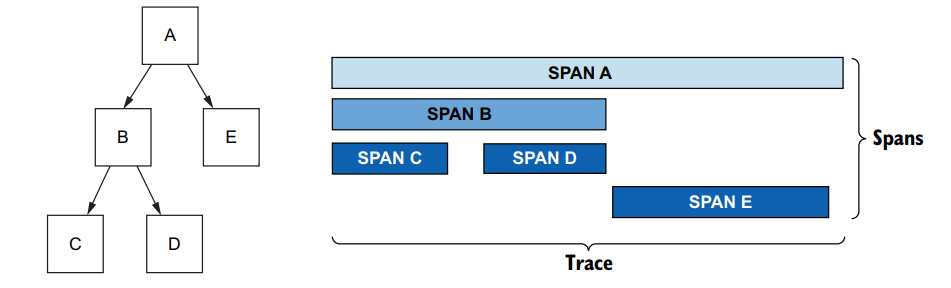
\includegraphics[width=1\linewidth]{Pics/2.3.2-p2}
			\caption{Mô hình span và trace}
			\label{fig:2}
		\end{figure}
		
		Istio có thể xử lý việc gửi các span tới công cụ theo dõi phân tán, vì vậy bạn không cần các thư viện dành riêng cho ngôn ngữ và cấu hình dành riêng cho ứng dụng để thực hiện việc này. Khi một request đi qua proxy, một trace mới sẽ được bắt đầu nếu không có request nào đang diễn ra, đồng thời thời gian bắt đầu và kết thúc của request được ghi lại như một phần của Span. Istio thêm các HTTP header, được gọi là Zipkin tracing header, vào request có thể được sử dụng để tương quan các đối tượng Span tiếp theo với Trace. Nếu một request đến với một dịch vụ và proxy Istio nhận ra các header, thì proxy sẽ coi đó là Trace đang diễn ra và không cố gắng tạo một Trace mới. Các Zipkin tracing header sau đây được sử dụng bởi Istio và chức năng theo dõi phân tán:
		
		\begin{itemize}				
			\item x-request-id
			\item x-b3-traceid
			\item x-b3-spanid
			\item x-b3-parentspanid
			\item x-b3-sampled
			\item x-b3-flags
			\item x-ot-span-context
		\end{itemize}
		
		Để chức năng theo dõi phân tán do Istio cung cấp hoạt động, mỗi ứng dụng cần thêm các header này tới bất kỳ request nào mà gọi đi nào mà nó thực hiện. Lý do là Istio không thể biết đâu là request đi và đâu là request đến.
		
	\section{Bảo mật các Microservices bằng Istio}
		{\hspace{0.6cm}Bảo mật ứng dụng bao gồm tất cả các hoạt động góp phần bảo vệ dữ liệu ứng dụng có giá trị quan trọng và không bị xâm phạm, đánh cắp hoặc truy cập trái phép bởi người dùng trái phép. Để bảo vệ dữ liệu người dùng, các quản trị viên cần:}
		\begin{itemize}
			\item Xác thực và ủy quyền của người dùng trước khi cho phép truy cập vào tài nguyên.
			\item Mã hóa dữ liệu khi truyền để ngăn không cho dữ liệu bị nghe trộm trong khi truyền qua nhiều thiết bị mạng để tiếp cận khách hàng yêu cầu dữ liệu.
		\end{itemize}
		
		\subsection{Bảo mật trong kiến trúc monoliths và kiến trúc microservices}
			{\hspace{0.6cm}Cả microservice và monolith đều cần triển khai xác thực và ủy quyền giữa người dùng cuối và dịch vụ với dịch vụ. Tuy nhiên, các microsevice có nhiều kết nối hơn và nhiều request di chuyển trong mạng. Ngược lại, monolith có ít kết nối hơn và thường được chạy trên cơ sở hạ tầng tĩnh hơn như máy ảo hoặc máy vật lý. Việc chạy trong cơ sở hạ tầng tĩnh làm cho địa chỉ IP trở thành một nguồn nhận dạng tốt và vì lý do đó, chúng thường được sử dụng trong các chứng chỉ để xác thực (cũng như các quy tắc tường lửa mạng).}
			
			Mặt khác, các microservice dễ dàng phát triển thành hàng trăm, hàng nghìn dịch vụ, khiến việc vận hành các dịch vụ trong môi trường tĩnh rất khó quản trị. Vì lý do này, các doanh nghiệp thường sử dụng dịch vụ điện toán đám mấy (ECS, EKS, AKS, ...) hoăc là các container orchestration (Docker Swarm, Nomad, Kubernetes, ...), nơi các dịch vụ được lên lịch cho nhiều máy chủ và các microserice thường có vòng đời ngắn. Điều này làm cho các phương pháp truyền thống như sử dụng địa chỉ IP trở thành nguồn nhận dạng không đáng tin cậy. Tệ hơn nữa, các dịch vụ không nhất thiết phải chạy trong cùng một mạng và có thể trải rộng trên các nhà cung cấp dịch vụ điện toán đám mây khác nhau và thậm chí chạy các cụm máy vật lý.
			
			Để giải quyết những thách thức này và cung cấp danh tính cho các microserice, Istio sử dụng đặc tả SPIFFE. SPIFFE là một tập hợp các tiêu chuẩn nguồn mở để cung cấp danh tính cho khối lượng công việc trong các môi trường không đồng nhất và năng động cao.
			
			SPIFFE là một URI tuân thủ RFC 3986 được tạo ở định dạng spiffe://trust-domain/path, trong đó:
			\begin{itemize}
				\item trust-domain đại diện cho nhà phát hành danh tính, chẳng hạn như một cá nhân hoặc tổ chức.
				\item path xác định duy nhất một khối lượng công việc trong trust-domain
			\end{itemize}
		
			Chi tiết về cách đường dẫn xác định khối lượng công việc được quyết định bởi SPIFFE. Istio điền vào đường dẫn này bằng cách sử dụng tài khoản dịch vụ mà theo đó một khối lượng công việc cụ thể sẽ chạy. Danh tính SPIFFE này được mã hóa trong chứng chỉ X.509, còn được gọi là Tài liệu nhận dạng có thể xác minh SPIFFE (SPIFFE Verifiable Identity Document), mà Istio control plane tạo ra cho khối lượng công việc. Các chứng chỉ này sau đó được sử dụng để mã hóa các đường truyền khi các dịch vụ kết nối với nhau.
		
		\subsection{Cách Istio bảo mật các microsevice}
			{\hspace{0.6cm}Istio có ba thành phần sau dùng để cấu hình Istio proxy để thực hiện các chức năng bảo mật:}
			\begin{itemize}
				\item Tài nguyên PeerAuthentication định cấu hình proxy để xác thực lưu lượng dịch vụ đến dịch vụ. Khi xác thực thành công, proxy sẽ trích xuất thông tin được mã hóa trong chứng chỉ và cung cấp thông tin đó để cho phép gửi các request.
				\item Tài nguyên RequestAuthentication định cấu hình proxy để xác thực thông tin đăng nhập của người dùng cuối đối với các máy chủ đã cấp chúng. Khi xác thực thành công, nó cũng trích xuất thông tin được mã hóa trong thông tin xác thực và cung cấp thông tin đó để cho phép gửi các request.
				\item Tài nguyên AuthorizationPolicy định cấu hình proxy để cho phép hoặc từ chối các thực hiện các request bằng cách đưa ra quyết định dựa trên dữ liệu được trích xuất bởi hai tài nguyên trước đó.
			\end{itemize}
		
		\subsection{Xác thực và mã hóa đường truyền giữa các Microservices với Istio}
			{\hspace{0.6cm}Theo mặc định, lưu lượng truy cập giữa các dịch vụ đã chèn proxy sidecar được mã hóa và xác thực lẫn nhau. Việc có một quy trình tự động phát hành và tạo mới chứng chỉ là rất quan trọng bởi vì theo lịch sử, quy trình này rất dễ xảy ra lỗi khi được quản lý bởi con người. Điều này gây ra những lần ngừng hoạt động không cần thiết và tốn kém mà lẽ ra có thể tránh được bằng cách sử dụng quy trình tự động, chẳng hạn như quy trình do Istio triển khai. Hình dưới đây cho thấy cách các dịch vụ sử dụng chứng chỉ do Istio control plane khiển cấp để xác thực lẫn nhau và mã hóa lưu lượng theo mặc định.}
			
			\begin{figure}[h]
				\centering
				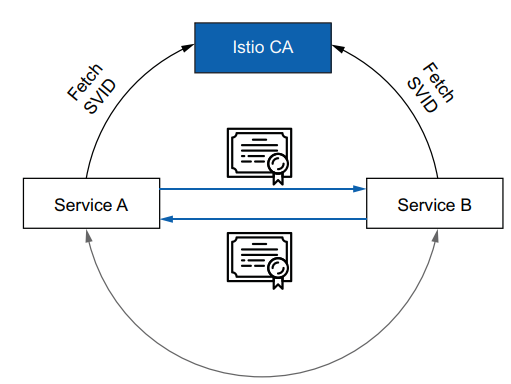
\includegraphics[width=0.7\linewidth]{Pics/2.4.3-p1}
				\caption{Các microservice xác thực lẫn nhau bằng cách sử dụng chứng chỉ SVID do cơ quan cấp chứng chỉ Istio cấp }
				\label{fig:2}
			\end{figure}
			
			Tài nguyên PeerAuthentication cấu hình các microserivce bắt buộc sử dụng mTLS hoặc chấp nhận các đường truyền không được mã hóa, có hai chế độ xác thực chính là STRICT (bắt buộc sử dụng mTLS) hoặc PERMISSIVE (có thể sử dụng mTLS hoặc không dùng mTLS). Và chế độ xác thực này có thể được cấu hình với nhiều phạm vi khác nhau như:
			
			\begin{itemize}
				\item Áp dụng chính sách xác thực của PeerAuthentication lên tất cả các microservice.
				\item Áp dụng chính sách xác thực của PeerAuthentication lên các microservice trên một namespace được chỉ định
				\item Áp dụng chính sách xác thực của PeerAuthentication lên các microservice được chỉ định cụ thể
			\end{itemize}
			 
			
		\subsection{Phân quyền cho các Microservices với Istio}
			{\hspace{0.6cm}Ủy quyền là quy trình xác định xem chủ thể được xác thực có được phép thực hiện một thao tác hay không, chẳng hạn như truy cập, chỉnh sửa hoặc xóa tài nguyên. Các chính sách được hình thành cùng với chủ thể được xác thực (“ai”) và ủy quyền (“cái gì”) và xác định ai có thể làm gì.}
			
			Istio cung cấp tài nguyên AuthorizationPolicy, là API khai báo để xác định các chính sách truy cập trên tất cả các microsevice, hoặc một số microservice trên một namespace cụ thể, hoặc một microservice cụ thể.
			
			Proxy dịch vụ được triển khai với mỗi dịch vụ là công cụ ủy quyền hoặc thực thi vì nó chứa tất cả các chính sách để xác định liệu một yêu cầu nên bị từ chối hay cho phép. Do đó, kiểm soát truy cập trong Istio cực kỳ hiệu quả vì các quyết định được đưa ra trực tiếp trong proxy. Proxy được định cấu hình với tài nguyên AuthorizationPolicy, tài nguyên này xác định các chính sách. Ví dụ:
			
			\begin{lstlisting}
			apiVersion: "security.istio.io/v1beta1"
			kind: "AuthorizationPolicy"
			metadata:
			  name: "allow-catalog-requests-in-web-app"
			  namespace: istioinaction
			spec:
			  selector:
			    matchLabels:
				  app: webapp
			  action: ALLOW
			  rules:
			  - to:
				- operation:
				    paths: ["/api/catalog*"]
			\end{lstlisting}
			
			Khi istiod khi nhận được AuthorizationPolicy mới đã được áp dụng cho cụm, nó sẽ xử lý và cập nhật các luật của AuthorizationPolicy vào các proxy của các microservice.
			
			AuthorizationPolicy cung cấp ba trường để định cấu hình và xác định chính sách:
			
			\begin{itemize}
				\item Trường selector xác định tập hợp các tài nguyên được áp dụng luật.
				\item Trường action có ba lựa chọn là ALLOW (cho phép), DENY (từ chối), hoặc là CUSTOM (tùy chỉnh). Các hành động sẽ chỉ được áp dụng nếu một trong các thành phần của trường rules giống với request.
				\item Trường rules xác định danh sách quy tắc xác request có bị vi phạm với quy tắc không và từ đó sẽ kích hoạt các chính sách như cho phép(ALLOW) hoặc chặn (DENY).
			\end{itemize}
		
			Trường rules còn có nhiều trường khác như:
			\begin{enumerate}
				\item[$\blacksquare$] Trường from chỉ định nguồn của yêu cầu, có thể là một trong các loại sau:
				\begin{itemize}
					\item principals: Một danh sách các định danh nguồn (SPIFFE ID)
					\item namespaces: Một danh sách các namespace.
					\item ipBlocks: Một địa chỉ IP hoặc một dải địa chỉ IP.
				\end{itemize}
				\item[$\blacksquare$] Trường to chỉ định các hoạt động của request, chẳng hạn như máy chủ hoặc phương thức của request.
				\item[$\blacksquare$] Trường when chỉ định danh sách các điều kiện cần phải đáp ứng sau khi quy tắc đã khớp.
			\end{enumerate}
			
			Sự phức tạp của các chính sách phát sinh khi nhiều chính sách được áp dụng cho các microservice và rất khó để phân biệt luật nào được ưu tiên trước. Nhiều giải pháp sử dụng trường ưu tiên để xác định quyền nào được ưu tiên hơn. Istio sử dụng một cách tiếp cận khác để đánh giá các chính sách:
			
			\begin{enumerate}
				\item[$\blacksquare$] CUSTOM được ưu tiên đầu tiên.
				\item[$\blacksquare$] DENY được ưu tiên thứ hai nếu không có CUSTOM.
				\item[$\blacksquare$] ALLOW được ưu tiên tiếp theo.
				\item[$\blacksquare$] Nếu có chính sách áp dụng lên tất cả các microservice hoặc không có chính sách nào áp dụng lên tất cả các microservice thì sẽ xảy ra hai trường hợp sau:
				\begin{itemize}
					\item Nếu có chính sách áp dụng lên tất cả các microservice, thì chính sách đó quyết định request đó dược chấp nhận hay không.
					\item Nếu không chính sách áp dụng lên tất cả các microservice, thì request sẽ:
					\begin{enumerate}
						\item[a.] được cho phép nếu không có chính sách ALLOW nào.
						\item[b.] sẽ từ chối nếu có chính sách ALLOW nhưng request không khớp với luật của ALLOW.
					\end{enumerate}
				\end{itemize}
			\end{enumerate}
	\newpage		
	\section*{Kết luận chương 2}
		{\hspace{0.6cm}Các ứng dụng hiện đại thường được kiến trúc dưới dạng tập hợp vi dịch vụ phân tán, với mỗi tập hợp microservice thực hiện một số chức năng riêng biệt. Service-mesh là lớp cơ sở hạ tầng chuyên dụng có thể thêm vào ứng dụng. Nó cho phép quản trị viên có thêm các khả năng như khả năng quan sát, quản lý lưu lượng và bảo mật một cách rõ ràng mà không cần phải sửa lại code của ứng dụng. }
		
		Khi việc triển khai các dịch vụ phân tán, chẳng hạn như trong hệ thống dựa trên Kubernetes, tăng về quy mô và độ phức tạp, việc hiểu và quản lý có thể trở nên khó khăn hơn. Các yêu cầu của nó có thể bao gồm phát hiện, cân bằng tải, khôi phục lỗi, số liệu và giám sát. Lưới dịch vụ cũng thường giải quyết các yêu cầu hoạt động phức tạp hơn, như thử nghiệm A/B, triển khai canary, giới hạn tốc độ, kiểm soát truy cập, mã hóa và xác thực đầu cuối.
		
		Giao tiếp giữa dịch vụ với dịch vụ là điều làm cho ứng dụng phân tán trở nên khả thi. Định tuyến giao tiếp cả bên trong và trên các cụm ứng dụng ngày càng trở nên phức tạp khi số lượng dịch vụ tăng lên.
		
		Istio có thể giải quyết các vấn để trên. Các tính năng mạnh mẽ của Istio cung cấp một cách thống nhất và hiệu quả hơn để bảo mật, kết nối và giám sát các dịch vụ. Istio là đường dẫn đến cân bằng tải, xác thực dịch vụ với dịch vụ và giám sát – với ít hoặc không có thay đổi mã dịch vụ.
		
\chapter{Triển khai Istio trên Kubernetes}
	\section{Mô hình triển khai}
	\subsection{Mô hình hạ tầng triển khai}
	Sử dụng máy tính hệ điều hành Windows, công cụ hỗ trợ ảo hóa cho hệ điều hành này là Hyper-V. Sau đó cài đặt Docker Desktop, trong Docker Desktop chúng ta sẽ cài đặt Docker Kubernetes. Cụm Docker Kubernetes sẽ có chỉ có một node làm Master Node và cũng đồng thời làm Worker Node, với địa chỉ IP của node là địa chỉ có máy Windows.
	
	\begin{figure}[h]
		\centering
		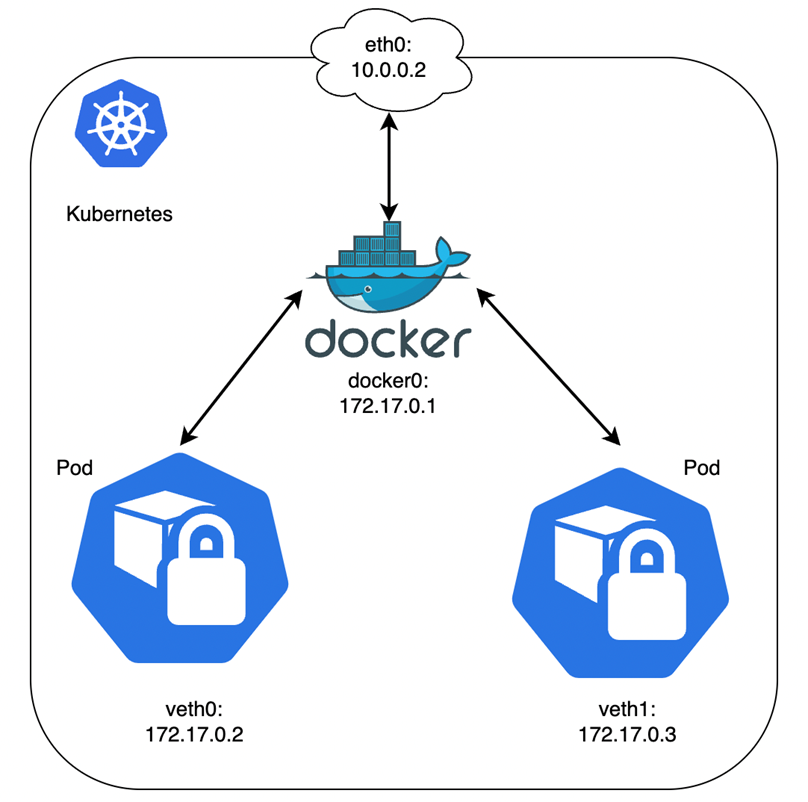
\includegraphics[width=0.7\linewidth]{Pics/3.1.1-1}
		\caption{Mô hình hạ tầng triển khai}
		\label{fig:3.1.1-1}
	\end{figure}
	\newpage
	\subsection{Mô hình Microservices}
	Mô hình ở đây là là một ứng dụng Bookinfo hiển thị thông tin về một cuốn sách, chứa mô tả về sách, chi tiết về sách (ISBN, số trang, v.v.) và một số bài đánh giá về sách.
	Ứng dụng Bookinfo được chia thành bốn dịch vụ nhỏ riêng biệt:
	\begin{itemize}
		\item \textit{productpage}. Microservice của productpage gọi các microservice details và reviews để điền vào trang hiển thị.
		\item \textit{details}.  Microservice details chứa thông tin sách.
		\item \textit{reviews}. Microservice reviews chứa các bài đánh giá sách.
		\item \textit{ratings}. Microservice ratings chứa thông tin xếp hạng và bài đánh giá về sách.
	\end{itemize}
	
	Có 3 phiên bản của Microservice \textit{reviews}:
	\begin{itemize}
		\item \textbf{Version 1} không gọi dịch vụ \textit{ratings}
		\item \textbf{Version 2} gọi dịch vụ \textit{ratings} và hiển thị các phần xếp hạng dưới dạng từ 1 đến 5 sao đen.
		\item \textbf{Version 3} gọi dịch vụ \textit{ratings} và hiển thị các phần xếp hạng dưới dạng từ 1 đến 5 sao đỏ.
	\end{itemize}
	
	Hình 3.2 diễn tả mô hình của dịch vụ trên.
	\begin{figure}[h]
		\centering
		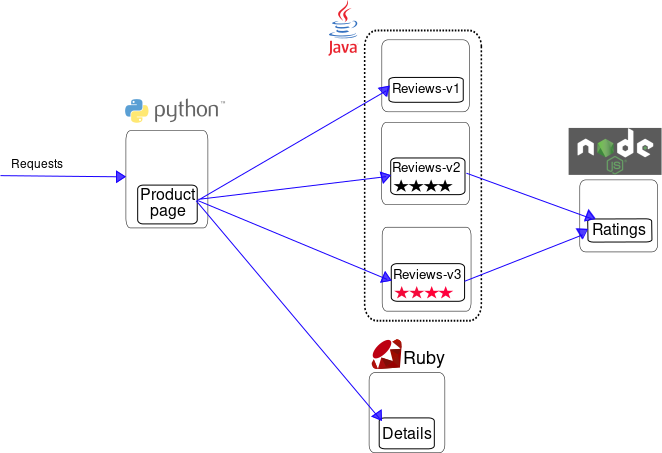
\includegraphics[width=0.7\linewidth]{Pics/3.1.2-1}
		\caption{Mô hình Microservices}
		\label{fig:3.1.2-1}
	\end{figure}
	\section{Cài đặt và thiết lập môi trường}
	Thực hiện quá trình cài đặt theo các bước:\\
	\textbf{Bước 1:} Cài đặt Docker Kubernetes\\
	Docker Kubernetes là một cụm đặc biệt trong kubernetes, chỉ có duy nhất một node, ngoài ra còn giúp chúng ta học tập và nghiện cứu phát triển kubernetes dễ dàng hơn. Trong phạm vi đề tài này, chúng ta sử dụng Docker Kubernetes để thực hiện nghiên cứu và phát triển các chính sách an toàn bằng istio. Trong Docker Desktop chúng ta vào Settings, chọn vào Kubernetes, tích vào Kubernetes và chờ Docker Desktop  cài đặt Docker Kubernetes.
	
	\begin{figure}[h!]
		\centering
		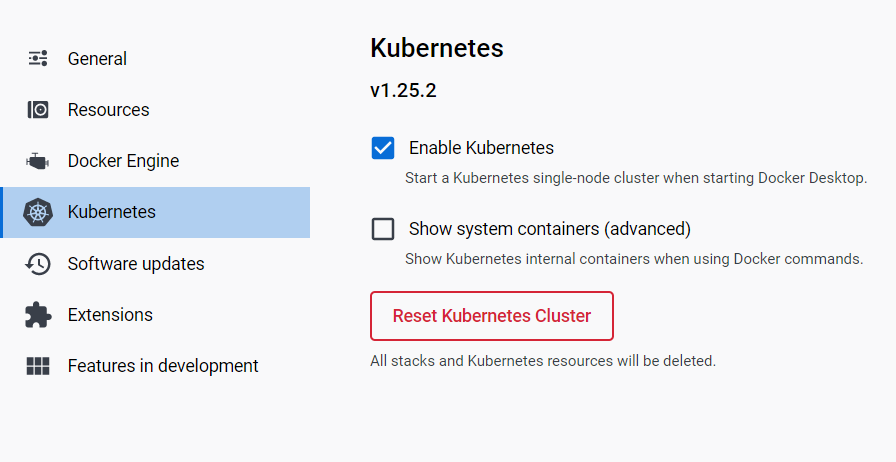
\includegraphics[width=0.65\linewidth]{Pics/3.2-1}
		\caption{Cài đặt Docker Kubernetes}
		\label{fig:3.2-1}
	\end{figure}
	
	\textbf{Bước 2:} Kiểm tra cụm Docker Kubernetes đã khởi động chưa
	\begin{lstlisting}
		$ kubectl get node
		NAME             STATUS   ROLES           AGE     VERSION
		docker-desktop   Ready    control-plane   2d14h   v1.25.2
	\end{lstlisting}
	\textbf{Bước 3:} Cài đặt Kubectl và Istioctl thông qua chocolatey
	Cài đặt Chocolatey thông qua Powershell
	\begin{lstlisting}
		Set-ExecutionPolicy Bypass -Scope Process -Force; [System.Net.ServicePointManager]::SecurityProtocol = [System.Net.ServicePointManager]::SecurityProtocol -bor 3072; iex ((New-Object System.Net.WebClient).DownloadString('https://community.chocolatey.org/install.ps1'))
	\end{lstlisting}
	
	Cài đặt Kubectl và Istioctl bằng Chocolatey
	\begin{lstlisting}
		$ choco install kubernetes-cli
		
		$ choco install istioctl
	\end{lstlisting}
	\textbf{Bước 4:} Cài đặt Istio
	\begin{lstlisting}
		$ istioctl install --set profile=demo -y
		Istio core installed
		Istiod installed
		Ingress gateways installed
		Egress gateways installed
		Installation complete                                                        
	\end{lstlisting}
	\textbf{Bước 5:} Kiểm tra Istio đã được cài đặt trên cụm chưa
	\begin{lstlisting}
		$ kubectl get pod -n istio-system
		NAME                                    READY   STATUS    RESTARTS      AGE
		istio-egressgateway-79598956cf-4vc6k    1/1     Running   2 (18m ago)   2d14h
		istio-ingressgateway-854c9d9c5f-h8xpl   1/1     Running   2 (18m ago)   2d14h
		istiod-fd94754fb-46mdd                  1/1     Running   2 (18m ago)   2d14h
	\end{lstlisting}
	\textbf{Bước 6:} Cài đặt namespace istioinaction cho các service 
	\begin{lstlisting}
		kubectl create namespace istioinaction
		namespace/istioinaction created
	\end{lstlisting}
	\textbf{Bước 7:} Inject istio vào namespace istioinaction
	\begin{lstlisting}
		$ kubectl label namespace istioinaction istio-injection=enabled
		namespace/istioinaction labeled
	\end{lstlisting}
	\textbf{Bước 8:} Triển khai ứng dụng 
	\begin{lstlisting}
		$ kubectl apply -f samples/bookinfo/platform/kube/bookinfo.yaml
		service/details created
		serviceaccount/bookinfo-details created
		deployment.apps/details-v1 created
		service/ratings created
		serviceaccount/bookinfo-ratings created
		deployment.apps/ratings-v1 created
		service/reviews created
		serviceaccount/bookinfo-reviews created
		deployment.apps/reviews-v1 created
		deployment.apps/reviews-v2 created
		deployment.apps/reviews-v3 created
		service/productpage created
		serviceaccount/bookinfo-productpage created
		deployment.apps/productpage-v1 created
	\end{lstlisting}
	\textbf{Bước 9:} Kiểm tra sự sẵn sàng cảu các pod cũng như Istio sidecar đã được đính kèm hay chưa
	\begin{lstlisting}
		$ kubectl get services
		NAME          TYPE        CLUSTER-IP       EXTERNAL-IP   PORT(S)    AGE
		details       ClusterIP   10.100.195.223   <none>        9080/TCP   2d20h
		kubernetes    ClusterIP   10.96.0.1        <none>        443/TCP    2d20h
		productpage   ClusterIP   10.108.125.43    <none>        9080/TCP   2d20h
		ratings       ClusterIP   10.104.36.197    <none>        9080/TCP   2d20h
		reviews       ClusterIP   10.102.245.160   <none>        9080/TCP   2d20h
		
		$ kubectl get pod
		NAME                             READY   STATUS    RESTARTS      AGE
		details-v1-5ffd6b64f7-tn8lc      2/2     Running   8 (12m ago)   2d20h
		productpage-v1-979d4d9fc-d8hsl   2/2     Running   8 (12m ago)   2d20h
		ratings-v1-5f9699cfdf-tsg85      2/2     Running   8 (12m ago)   2d20h
		reviews-v1-569db879f5-q6v49      2/2     Running   8 (12m ago)   2d20h
		reviews-v2-65c4dc6fdc-2w95m      2/2     Running   8 (12m ago)   2d20h
		reviews-v3-c9c4fb987-x85tw       2/2     Running   8 (12m ago)   2d20h
	\end{lstlisting}
	\textbf{Bước 10:} Xác nhận ứng dụng Bookinfo đang chạy thông qua gửi các yêu cầu bằng lệnh {\color{red}curl} 
	\begin{lstlisting}
		$ kubectl exec "$(kubectl get pod -l app=ratings -o jsonpath='{.items[0].metadata.name}')" -c ratings -- curl -sS productpage:9080/productpage | grep -o "<title>.*</title>"
		<title>Simple Bookstore App</title>
	\end{lstlisting}
	\textbf{Bước 11:} Đặt ingress IP và port
	\begin{lstlisting}
		$ kubectl apply -f samples/bookinfo/networking/bookinfo-gateway.yaml
		gateway.networking.istio.io/bookinfo-gateway created
		virtualservice.networking.istio.io/bookinfo created
		
		$ kubectl get gateway
		NAME               AGE
		bookinfo-gateway   2d20h
	\end{lstlisting}
	\textbf{Bước 12:} Kiểm tra xem ứng dụng đã được truy cập được từ ngoài Cluster hay chưa
	\begin{lstlisting}
		$ curl -s "http://localhost/productpage" | grep -o "<title>.*</title>"
		<title>Simple Bookstore App</title>
	\end{lstlisting}
	\section{Thực nghiệm}
			\subsection{Canary Release}
		\subsubsection{a. Mục đích}
		Có nhiều chiến lược triển khai (deployment strategy) được áp dụng khi đưa một phiên bản mới của ứng dụng lên môi trường thực tế (production). Các chiến lược triển khai phổ biến là recreate, ramped, blue/green, canary, A/B testing, shadow… Mỗi chiến lược triển khai đều có điểm mạnh và yếu riêng. Việc lựa chọn chiến lược nào sẽ tuỳ thuộc vào bài toán cụ thể của từng loại ứng dụng. Đối với một số services trong các Platform, mỗi rủi ro gặp phải khi triển khai ở môi trường Production sẽ có sự ảnh hưởng rất lớn đến toàn bộ hệ thống, cũng như trải nghiệm người dùng. Vậy nên, áp dụng các giải pháp an toàn cho các trường hợp này là ưu tiên hàng đầu và là điều quan trọng cần phải làm. Đảm bảo được zero downtime, giảm mức độ ảnh hưởng và có thể kịp thời rollback là tiêu chí hàng đầu trong việc chọn chiến lược triển khai.
		\begin{figure}[h]
			\centering
			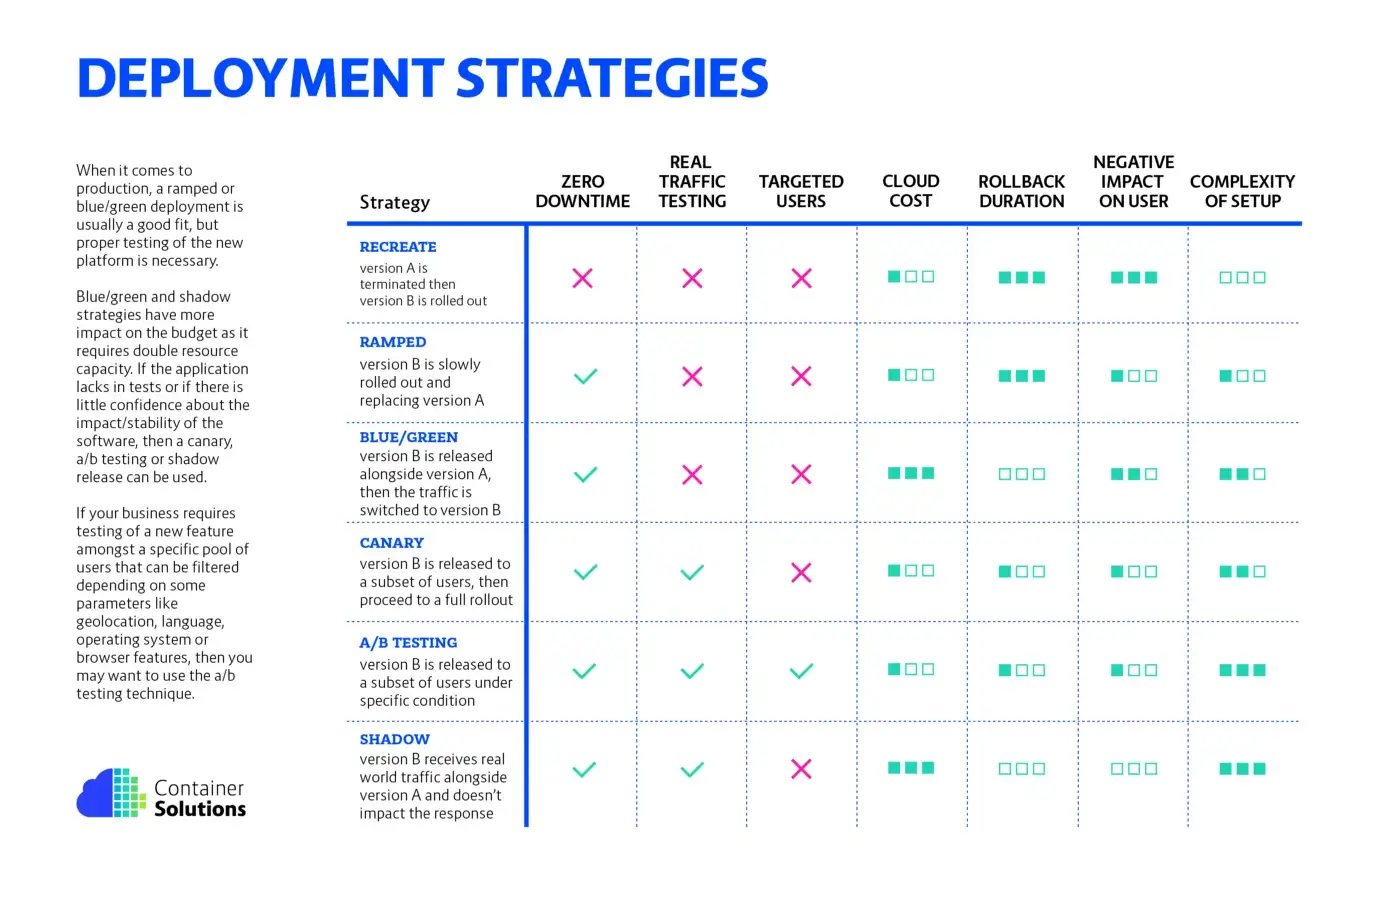
\includegraphics[width=0.7\linewidth]{Pics/3.3.1-1}
			\caption{Mỗi chiến lược triển khai đều có điểm mạnh và yếu riêng. Việc lựa chọn chiến lược nào sẽ tuỳ thuộc vào tình hình và bài toán cụ thể của từng loại ứng dụng}
			\label{fig:3.3-1}
		\end{figure}
		
		Canary là chiến lược triển khai từng phần. Khi phiên bản mới được triển khai (v2), các traffic sẽ được chuyển dần từ phiên bản cũ (v1) qua v2. Các traffic này sẽ được phân chia theo tỷ trọng (weight), tăng dần theo mỗi bước (step). Sau mỗi bước sẽ đánh giá chất lượng của v2 so với v1, việc đánh giá này tuỳ thuộc vào ngữ cảnh sẽ là tỉ lệ lỗi, hiệu năng (performance), độ trễ (latency). Với chiến lược đó, canary sẽ giúp kiểm soát tốt chất lượng của phiên bản mới, kịp thời đánh giá chất lượng và đưa ra quyết định chính xác khi xác nhận phiên bản mới (promote new version).
		
		\subsubsection{b. Kịch bản}
		Trong mô hình xây dựng một trang web "Bookinfo" đơn giản với chức năng "review" cùng với 3 phiên bản triển khai khác nhau. Với chiến lược triển khai từng phần của Canary, ta có thể chia làm 3 bước, giảm dần tỉ trọng các traffic, đồng thời tăng tỉ trọng các traffic vào v2/v3:
		\begin{itemize}
			\item \textbf{Bước 1:} 90\% request vào v1, 10\% request vào v2/v3
			\item \textbf{Bước 2:} 80\% request vào v1, 20\% request vào v2/v3
			\item \textbf{Bước 3:} 50\% request vào v1, 50\% request vào v2/v3
		\end{itemize}
		Sau mỗi bước sẽ kiểm tra số lượng các request bị lỗi (http code 5xx) và tốc độ phản hồi có đúng mục tiêu không (P99 dưới 500ms) bằng một số công cụ theo dõi sẽ trình bày trong phần tiếp theo. Nếu kết quả không như mong muốn sẽ đẩy các traffic vào v1 như cũ và loại bỏ v2. Nếu kết quả phù hợp thì sẽ quyết định sử dụng v2/v3 và loại bỏ v1.
		\subsubsection{c. Các bước thực hiện}
		Istio sử dụng các subset trong destination rules để xác định các phiên bản của dịch vụ. Vì thế trước hết ta phải tạo destination rule mặc định cho dịch vụ với việc triển khai toàn bộ các phiên bản.
		\begin{lstlisting}
			$ kubectl apply -f samples/bookinfo/networking/destination-rule-all.yaml
			
			$ for i in $(seq 1 10); do curl -s "http://localhost/productpage" | grep "review"; done
			<u>reviews-v3-c9c4fb987-x85tw</u>
			<u>reviews-v2-65c4dc6fdc-2w95m</u>
			<u>reviews-v1-569db879f5-q6v49</u>
			<u>reviews-v2-65c4dc6fdc-2w95m</u>
			<u>reviews-v2-65c4dc6fdc-2w95m</u>
			<u>reviews-v1-569db879f5-q6v49</u>
			<u>reviews-v1-569db879f5-q6v49</u>
			<u>reviews-v2-65c4dc6fdc-2w95m</u>
			<u>reviews-v3-c9c4fb987-x85tw</u>
			<u>reviews-v3-c9c4fb987-x85tw</u>
		\end{lstlisting}
		Như vậy qua việc dùng lệnh {\color{red}curl} ta có thể thấy được toàn bộ cả 3 phiên bản đều đã được triển khai thành công.
		Lúc này ta có thể bắt đầu quá trình Canary release.
		\textbf{Bước 1:} Ta định hướng với 90\% request vào v1, 10\% request vào v2
		\begin{lstlisting}
			$ kubectl apply -f .\samples\bookinfo\networking\virtual-service-reviews-90-10.yaml
			virtualservice.networking.istio.io/reviews created
			
			$ for i in $(seq 1 10); do curl -s "http://localhost/productpage" | grep "review"; done
			<u>reviews-v1-569db879f5-q6v49</u>
			<u>reviews-v1-569db879f5-q6v49</u>
			<u>reviews-v1-569db879f5-q6v49</u>
			<u>reviews-v1-569db879f5-q6v49</u>
			<u>reviews-v1-569db879f5-q6v49</u>
			<u>reviews-v1-569db879f5-q6v49</u>
			<u>reviews-v2-65c4dc6fdc-2w95m</u>
			<u>reviews-v1-569db879f5-q6v49</u>
			<u>reviews-v1-569db879f5-q6v49</u>
			<u>reviews-v1-569db879f5-q6v49</u>
		\end{lstlisting}
		Ở đây ta có thể thấy hầu hết các yêu cầu đề trả về v1, một số trả về v2 và không có v3
		Sau quá trình theo dõi và thu thập số liệu trong quá trình triển khai ta loại bỏ cấu hình trên để đến với các bước tiếp theo:
		\begin{lstlisting}
			$ kubectl delete -f .\samples\bookinfo\networking\virtual-service-reviews-90-10.yaml
			virtualservice.networking.istio.io "reviews" deleted
		\end{lstlisting}
		Tiếp theo ta thực hiện các bước 2 và 3 với cách thực hiện tương tự như trên để có được kết quả trả về với các ti lệ khác nhau.
		\begin{lstlisting}
			$ kubectl apply -f .\samples\bookinfo\networking\virtual-service-reviews-80-20.yaml
			virtualservice.networking.istio.io/reviews created
			
			$ for i in $(seq 1 10); do curl -s "http://localhost/productpage" | grep "review"; done
			<u>reviews-v2-65c4dc6fdc-2w95m</u>
			<u>reviews-v2-65c4dc6fdc-2w95m</u>
			<u>reviews-v1-569db879f5-q6v49</u>
			<u>reviews-v1-569db879f5-q6v49</u>
			<u>reviews-v1-569db879f5-q6v49</u>
			<u>reviews-v2-65c4dc6fdc-2w95m</u>
			<u>reviews-v2-65c4dc6fdc-2w95m</u>
			<u>reviews-v1-569db879f5-q6v49</u>
			<u>reviews-v2-65c4dc6fdc-2w95m</u>
			<u>reviews-v1-569db879f5-q6v49</u>
			
			$ kubectl delete -f .\samples\bookinfo\networking\virtual-service-reviews-80-20.yaml
			virtualservice.networking.istio.io "reviews" deleted
			###
			$ kubectl apply -f .\samples\bookinfo\networking\virtual-service-reviews-50-v3.yaml
			virtualservice.networking.istio.io/reviews created
			
			$ for i in $(seq 1 10); do curl -s "http://localhost/productpage" | grep "review"; done
			<u>reviews-v3-c9c4fb987-x85tw</u>
			<u>reviews-v3-c9c4fb987-x85tw</u>
			<u>reviews-v1-569db879f5-q6v49</u>
			<u>reviews-v3-c9c4fb987-x85tw</u>
			<u>reviews-v1-569db879f5-q6v49</u>
			<u>reviews-v3-c9c4fb987-x85tw</u>
			<u>reviews-v1-569db879f5-q6v49</u>
			<u>reviews-v3-c9c4fb987-x85tw</u>
			<u>reviews-v1-569db879f5-q6v49</u>
			<u>reviews-v3-c9c4fb987-x85tw</u>
			
			kubectl delete -f .\samples\bookinfo\networking\virtual-service-reviews-50-v3.yaml
			virtualservice.networking.istio.io "reviews" deleted
		\end{lstlisting}
		Như vậy, qua các bước trên có thể thực hiện triển khai toàn bộ v2 hay tiếp tục kiểm tra v3; Từ quá trình triển khai các phiên bản khác nhau với lưu lượng được kiểm soát ta có thể thử nghiệm các phiên bản mới mà không phải đối mặt với việc gây ảnh hưởng tới toàn bộ hệ thống khi chỉ 1 phiên bản có lỗi.
		\subsection{Kiali Dashboard}
		\subsubsection{a. Mục đích}
		Như có nói ở trên, để có thể kiểm tra giám sát quá trình triển khai thì chúng ta cần phải có một công cụ cung cấp khả năng theo dõi, giám sát, giúp chúng ta xem được network của ứng dụng microservice, kiểm tra request giữa từng service, response time,... Kiali là một công cụ giúp chúng ta thực hiện điều đó
		\subsubsection{b. Kịch bản}
		Ở đây ta dựng một Kiali Dashboard để có thể giám sát quá trình Canary release ở trên, kiểm soát các thông số đối với từng bản thử nghiệm để cho ra kết quả có triển khai phiên bản đó trên toàn bộ hệ thống hay không
		\subsubsection{c. Các bước thực hiện}
		Trước hết ta cài đặt Kiali cùng với add-on của nó
		\begin{lstlisting}
			$ kubectl apply -f .\samples\addons\kiali.yaml
			serviceaccount/kiali created
			configmap/kiali created
			clusterrole.rbac.authorization.k8s.io/kiali-viewer created
			clusterrole.rbac.authorization.k8s.io/kiali created
			clusterrolebinding.rbac.authorization.k8s.io/kiali created
			role.rbac.authorization.k8s.io/kiali-controlplane created
			rolebinding.rbac.authorization.k8s.io/kiali-controlplane created
			service/kiali created
			deployment.apps/kiali created
			
			$ kubectl apply -f .\samples\addons\prometheus.yaml
			serviceaccount/prometheus created
			configmap/prometheus created
			clusterrole.rbac.authorization.k8s.io/prometheus created
			clusterrolebinding.rbac.authorization.k8s.io/prometheus created
			service/prometheus created
			deployment.apps/prometheus created
		\end{lstlisting}
		Sau đó ta dùng câu lệnh {\color{red}Istioctl dashboard kiali} để mở Kiali dashboard trên trình duyệt web.
		\begin{figure}[h]
			\centering
			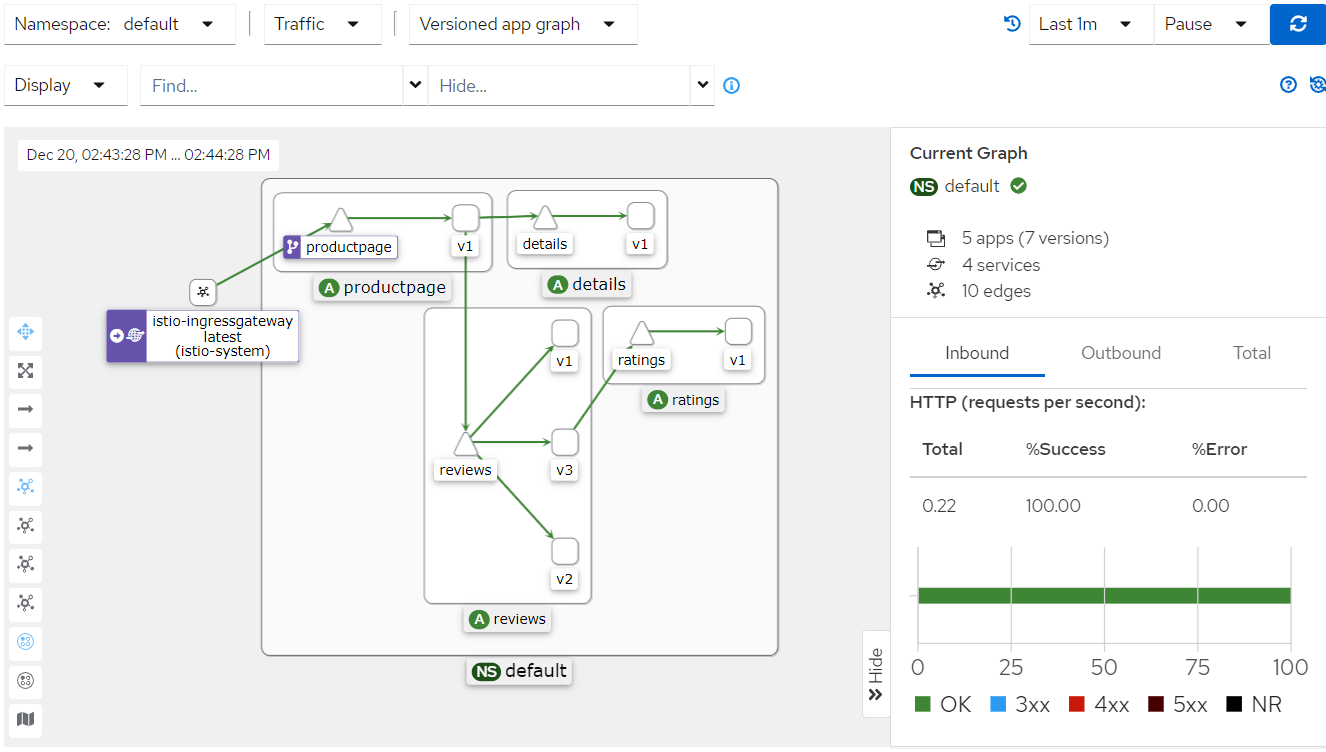
\includegraphics[width=0.7\linewidth]{Pics/3.3.2-1}
			\caption{Khởi động Kiali Dashboard}
			\label{fig:3}
		\end{figure}
		Khi này ở tab Graph cùng với thuộc tính Namespace default ta có thể thấy được quá trình triển khai của ứng dụng Bookinfo ở trên một cách trực tiếp và giúp ta có thể hình dung một cách rõ ràng nhất về quá trình hoạt động của dịch vụ.
		Thậm chí ta có thể theo dõi các chỉ số hoạt động chi tiết hơn nữa như Response time, Traffic rate,... 
		\begin{figure}[h]
			\centering
			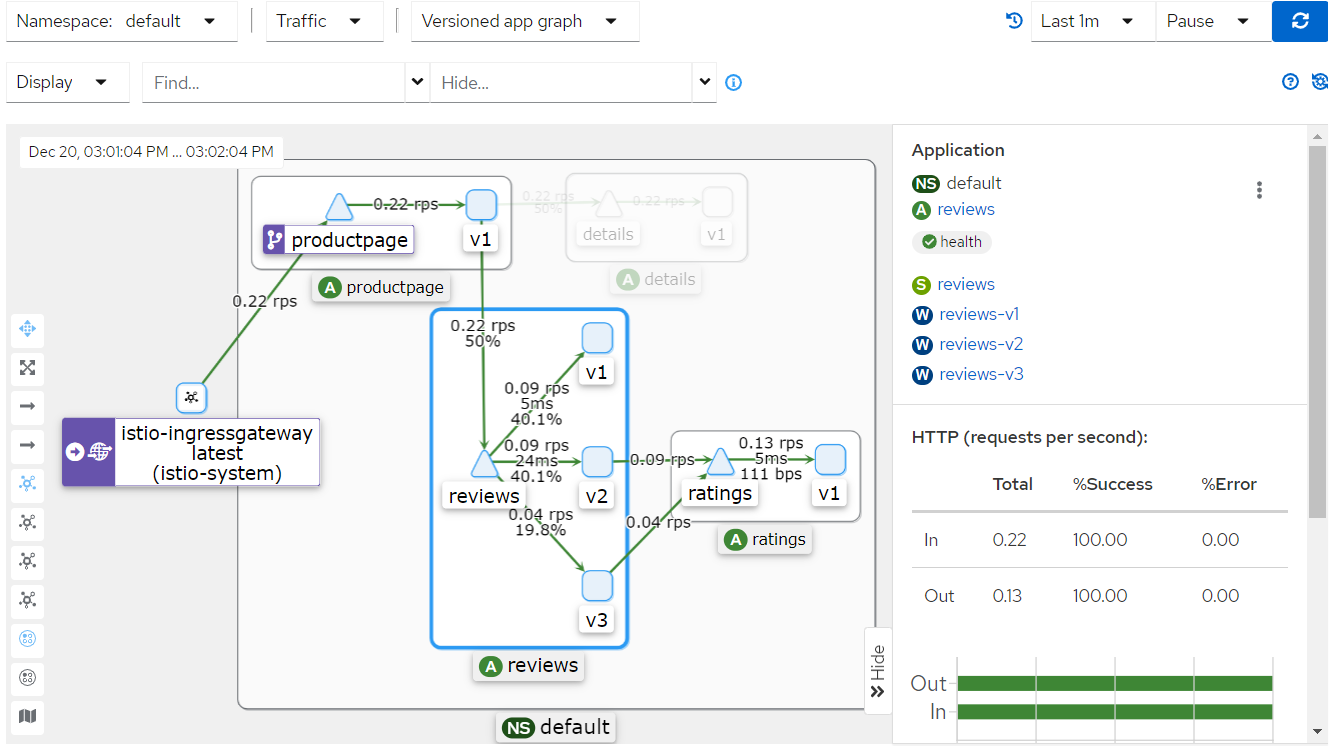
\includegraphics[width=0.7\linewidth]{Pics/3.3.2-2}
			\caption{Theo dõi các thông tin chi tiết trong Kiali Dashboard}
			\label{fig:3.4-2}
		\end{figure}
		
		Như trong hình 3.6 ta có thể thấy được thông tin về Traffic Distribution của ứng dụng "reviews" đối với từng phiên bản của nó, chẳng hạn như 40,1\% với v1 và v2 hay 19,8\% với v3. Ta cũng có thể thấy thời gian phản hồi lớn nhất của 99\% gói tin gửi giữa các thành phần trong hệ thống như ta thấy được thời gian phản hồi giữa ứng dụng "reviews" v2 với dịch vụ "reviews" là 24ms cũng như Traffic Rate giữa chúng là 0.09 request-per-second 
		\subsection{Xác thực và mã hóa đường truyền giữa các microservice}
			\subsubsection{a. Mục đích}
				{\hspace{0.6cm}Hai microservice sẽ được xác thực với nhau qua cơ chế mTLS và đường truyền giữa hai microservice cũng được mã hóa nhằm chống kẻ tấn công bắt trộm gói tin và đọc thông tin của những gói tin chưa được mã hóa giữa các microservice}
			\subsubsection{b. Kịch bản}
				\begin{enumerate}
					\item[$\blacksquare$] Tạo ra namespace sleep, sau đó tạo pod sleep trong namespace sleep.
					\item[$\blacksquare$] Từ trong pod sleep sử dụng câu lệnh curl đến pod productpage-v1.
					\item[$\blacksquare$] Áp dụng chính sách cấm tất các pod chưa được xác thực với các pod đã được xác thực.
					\item[$\blacksquare$] Sử dụng lại câu lệnh curl từ pod sleep đến pod productpage-v1.
					\item[$\blacksquare$] Sử dụng câu lệnh để bật tính năng tcpdump của proxy, sau đó xóa pod của productpage-v1 để proxy được tái tạo lại và có cơ chế tcpdump.
					\item[$\blacksquare$] Sử dụng câu lệnh tcpdump từ proxy của productpage-v1 và truy cập trang productpage từ trình duyệt. Sau đó quan sát màn hình proxy đang tcpdump thấy đường truyền được mã hóa. 
				\end{enumerate}
			\subsubsection{c. Các bước thực hiện}
				{\hspace{0.6cm}Bước 1: Tạo namspace sleep và pod sleep bằng câu lệnh sau:}
				\begin{lstlisting}
				$ kubectl create namespace sleep
				namespace/sleep created
				$ kubectl apply -f manifests/authentication/sleep.yaml -n sleep
				serviceaccount/sleep created
				service/sleep created
				deployment.apps/sleep created
				$ kubectl get pod -n sleep
				NAME                     READY   STATUS    RESTARTS   AGE
				sleep-787dbb8dd6-f25x2   1/1     Running   0          50s
				\end{lstlisting}
				
				Bước 2: Sử dụng câu lệnh curl trong pod sleep để gọi đến dịch vụ productpage bằng câu lệnh sau:
				\begin{lstlisting}
				$ kubectl -n sleep exec deploy/sleep -c sleep --  curl -s productpage.default:9080/productpage -o /dev/null -w "%{http_code}"
				200
				\end{lstlisting}
				
				Bước 3: Tạo ra file chính sách cấm tất cả các pod chưa được xác thực với các pod đã được xác thực, trong đó phần name bắt buộc phải có giá trị default và phần namespace bắt buộc là namespace của istiod được cài đặt, và mode là STRICT để bắt buộc tất cả mọi pod đã được cài Istio phải xác thực với nhau mới được kết nối
				\begin{lstlisting}
				apiVersion: "security.istio.io/v1beta1"
				kind: "PeerAuthentication"
				metadata:
				  name: "default"
				  namespace: "istio-system"
				spec:
			 	  mtls:
				    mode: STRICT 
				\end{lstlisting}
				
				Bước 4: Áp dụng chính sách và từ pod sleep thử curl lại dịch vụ productpage bằng câu lệnh sau:
				\begin{lstlisting}
				$ kubectl apply -f manifests/authentication/meshwide-strict-peer-authn.yaml 
				peerauthentication.security.istio.io/default configured
				$ kubectl -n sleep exec deploy/sleep -c sleep --  curl -s productpage.default:9080/productpage
				command terminated with exit code 56
				\end{lstlisting}
				
				Bước 5: Bật tính năng tcpdump của proxy, xóa pod productpage  bằng các câu lệnh dưới sau đó đợi pod mới được khởi tạo lại:
				\begin{lstlisting}
				$ istioctl install -y --set profile=demo --set values.global.proxy.privileged=true
				$ kubectl delete pod productpage-v1-979d4d9fc-87fdq
				pod "productpage-v1-979d4d9fc-87fdq" deleted
				\end{lstlisting}
				
				Bước 6: Sử dụng câu lệnh tcpdump trong proxy của pod productpage sau đó lên trên trình duyệt web truy cập vào địa chỉ http://localhost/productpage sau đó quay lại terminal đang thực hiện câu lệnh dump xem các request đang được mã hóa:
				\begin{lstlisting}
				$ kubectl  exec deploy/productpage-v1 -c istio-proxy -- sudo tcpdump -l --immediate-mode -vv -s 0  '(((ip[2:2] - ((ip[0]&0xf)<<2)) - ((tcp[12]&0xf0)>>2)) != 0)'
				tcpdump: listening on eth0, link-type EN10MB (Ethernet), capture size 262144 bytes
				05:43:37.964166 IP (tos 0x0, ttl 64, id 4024, offset 0, flags [DF], proto TCP (6), length 168)
				10.1.0.1.41546 > productpage-v1-979d4d9fc-55qgk.15021: Flags [P.], cksum 0x175a (incorrect -> 0x450f), seq 469286402:469286518, ack 2038184201, win 502, options [nop,nop,TS val 169039982 ecr 766623303], length 116
				05:43:37.964960 IP (tos 0x0, ttl 64, id 62383, offset 0, flags [DF], proto TCP (6), length 195)
				productpage-v1-979d4d9fc-55qgk.15021 > 10.1.0.1.41546: Flags [P.], cksum 0x1775 (incorrect -> 0x7159), seq 1:144, ack 116, win 509, options [nop,nop,TS val 766623304 ecr 169039982], length 143
				05:43:37.965590 IP (tos 0x0, ttl 64, id 20122, offset 0, flags [DF], proto UDP (17), length 67)
				productpage-v1-979d4d9fc-55qgk.35855 > kube-dns.kube-system.svc.cluster.local.domain: [bad udp cksum 0x1768 -> 0xf9ed!] 57182+ PTR? 1.0.1.10.in-addr.arpa. (39)
				05:43:37.972419 IP (tos 0x0, ttl 64, id 12075, offset 0, flags [DF], proto UDP (17), length 67)
				kube-dns.kube-system.svc.cluster.local.domain > productpage-v1-979d4d9fc-55qgk.35855: [bad udp cksum 0x1768 -> 0x796a!] 57182 NXDomain q: PTR? 1.0.1.10.in-addr.arpa. 0/0/0 (39)
				\end{lstlisting}
				
				
		\subsection{Ủy quyền giữa các microservice}
			\subsubsection{a. Mục đích}
			{\hspace{0.6cm}Istio không chỉ giúp quản trị viên xác thực các microservice, sau khi xác thực chúng ta có thể phân quyền cho các microservice, hạn chế microserivce chỉ có thể sử dụng một số tính năng cụ thể của microservice khác.}
			\subsubsection{b. Kịch bản}
			\begin{enumerate}
				\item[$\blacksquare$] Áp dụng chính sách cấm tất cả các requests đến với tất cả các pod trọng Kubernetes.
				\item[$\blacksquare$] Lên trình duyệt web truy cập đến dịch vụ thì thấy bị từ chối.
				\item[$\blacksquare$] Áp dụng chính sách cho phép request đến productpage-v1.
				\item[$\blacksquare$] Lên trình duyệt web truy cập đến dịch vụ productpage nhưng dịch vụ reviews, details, ratings bị lỗi.
				\item[$\blacksquare$] Áp dụng chính sách cho phép productpage-v1 có thể lấy thông tin từ dịch vụ details.
				\item[$\blacksquare$] Lên trình duyệt web truy cập đến dịch vụ productpage thấy dịch vụ details không bị lỗi nhưng dịch vụ reviews, ratings bị lỗi.
				\item[$\blacksquare$] Áp dụng chính sách cho phép productpage-v1 có thể lấy thông tin từ dịch vụ reviews.
				\item[$\blacksquare$] Lên trình duyệt web truy cập đến dịch vụ productpage thấy dịch vụ reviews không bị lỗi nhưng dịch vụ ratings bị lỗi.
				\item[$\blacksquare$] Áp dụng chính sách cho phép productpage-v1 có thể lấy thông tin từ dịch vụ ratings.
				\item[$\blacksquare$] Lên trình duyệt web truy cập đến dịch vụ productpage thấy các dịch vụ không bị lỗi. 
			\end{enumerate}
			\subsubsection{c. Các bước thực hiện}
				Bước 1: Tạo file chính sách như dưới trong đó trường namespace sẽ để là default, và spec là {}, có nghĩa là từ chối tất cả các request trong namespace default:
				\begin{lstlisting}
				apiVersion: security.istio.io/v1beta1
				kind: AuthorizationPolicy
				metadata:
				  name: allow-nothing
				  namespace: default
				spec:
				  {}
				\end{lstlisting}
						
				Bước 2: Sử dụng câu lệnh dưới để áp dụng file chính sách và truy cập lên trình duyệt web:
				\begin{lstlisting}
				$ kubectl apply -f manifests/authoriztion/deny-all.yaml 
				authorizationpolicy.security.istio.io/allow-nothing created
				\end{lstlisting}
				\begin{figure}[h]
					\centering
					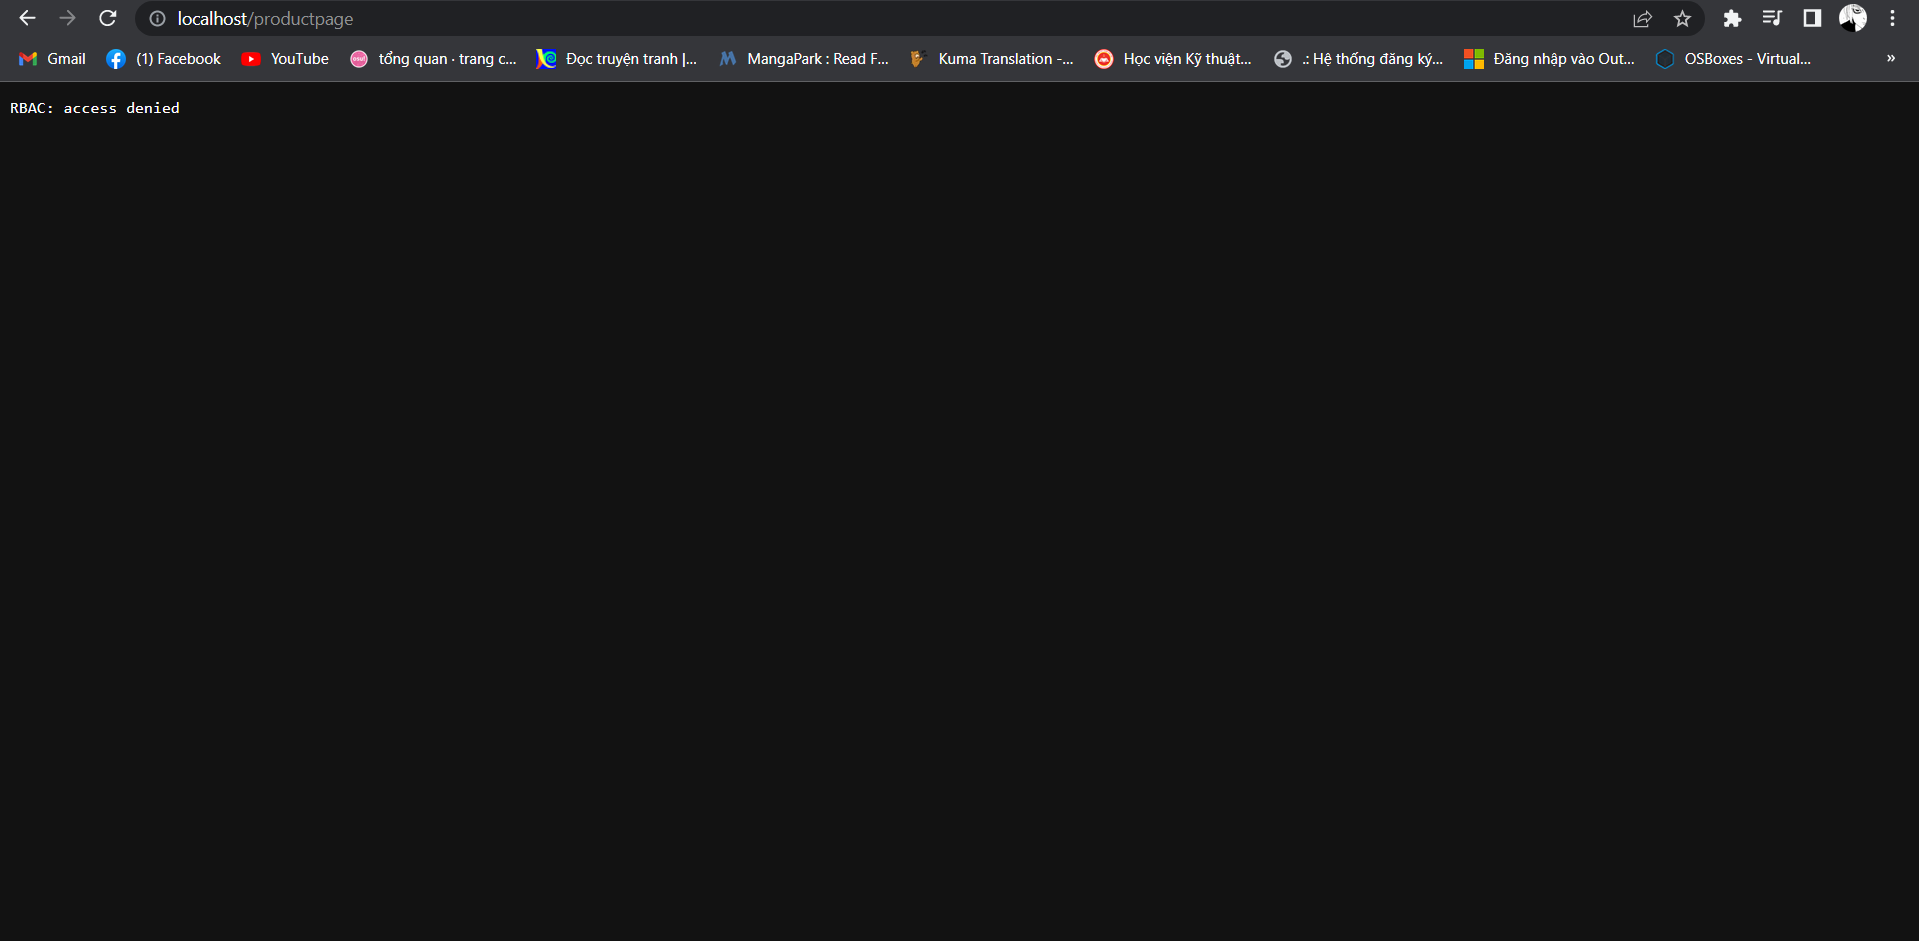
\includegraphics[width=1\linewidth]{Pics/3.3.2-p1}
					\caption{Không thể truy cập vào dịch vụ}
					\label{fig:3}
				\end{figure}
			
				Bước 3: Tạo file chính sách cho phép vào dịch vụ productpage như hình dưới, trong đó chúng ta để matchLabels là app: productpage và trường action là ALLOW, và method có thể sử dụng là GET. Nghĩa là tất các các app được đánh nhãn app có giá trị là productpage thì sẽ cho phép tất cả mọi dịch vụ hay người dùng sử dụng phương thức GET đối với dịch vụ này:
				\begin{lstlisting}
				apiVersion: security.istio.io/v1beta1
				kind: AuthorizationPolicy
				metadata:
				  name: "productpage-viewer"
				  namespace: default
				spec:
				  selector:
				    matchLabels:
				      app: productpage
				  action: ALLOW
				  rules:
				  - to:
				    - operation:
				        methods: ["GET"]
				\end{lstlisting}
				
				Bước 4: Sử dụng câu lệnh dưới để áp dụng file chính sách và truy cập lên trình duyệt web:
				\begin{lstlisting}
				$ kubectl apply -f manifests/authoriztion/allow-product-page.yaml 
				authorizationpolicy.security.istio.io/productpage-viewer created
				\end{lstlisting}
				\begin{figure}[h]
					\centering
					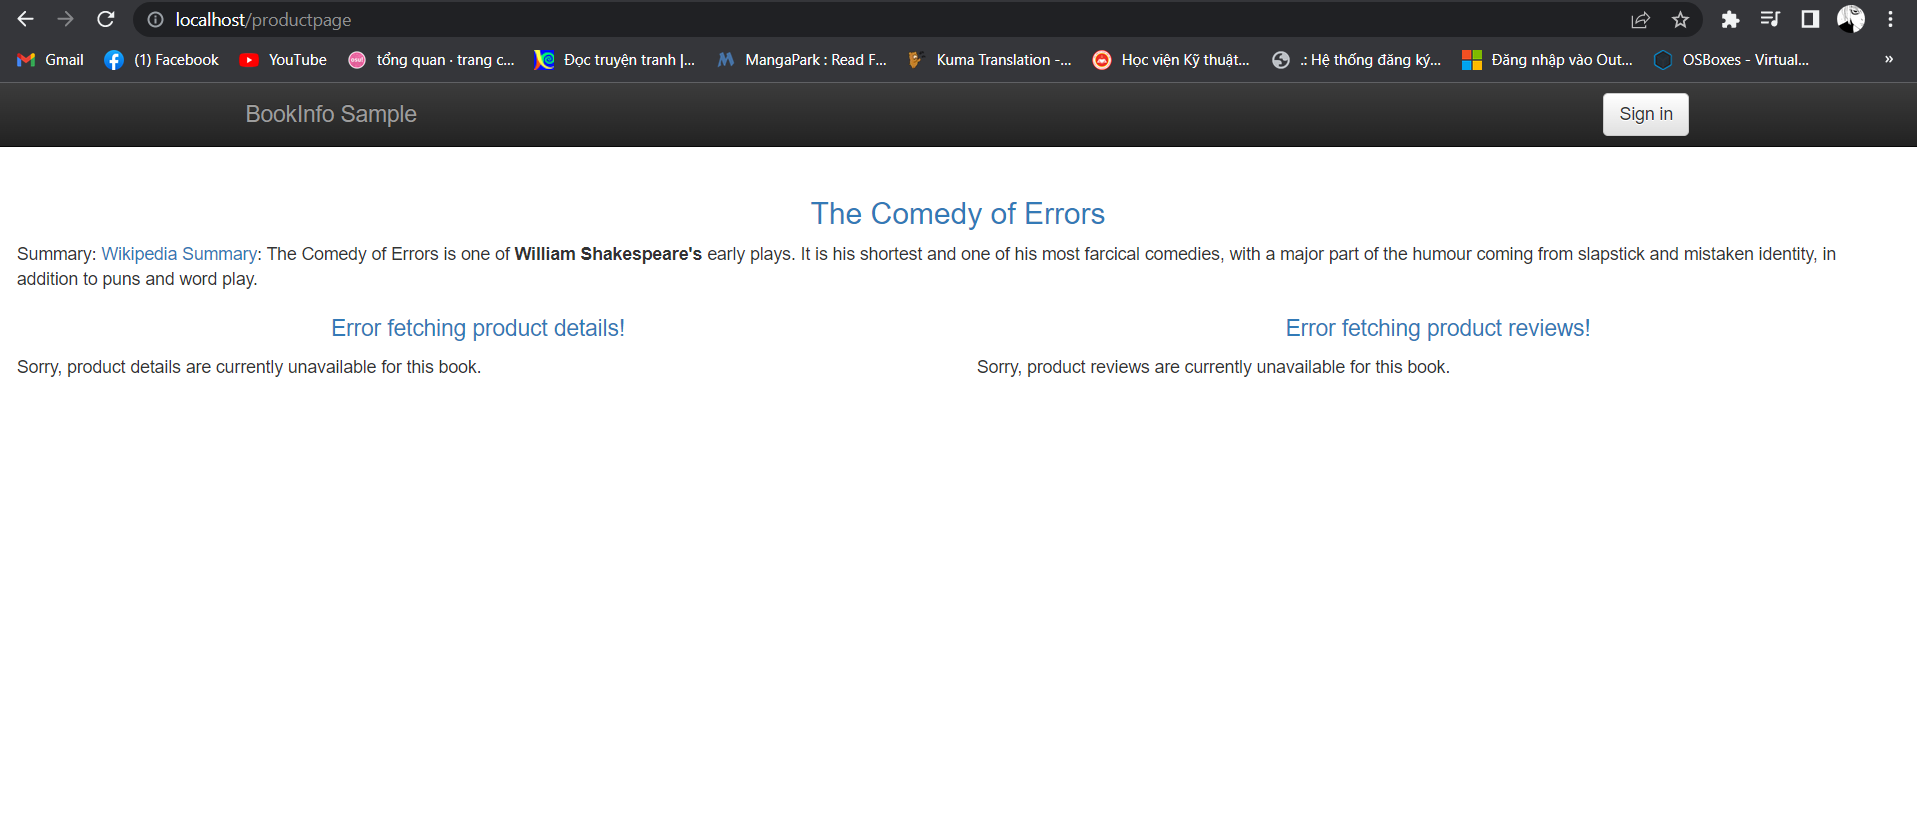
\includegraphics[width=0.7\linewidth]{Pics/3.3.2-p2}
					\caption{Đã vào được productpage nhưng các dịch vụ khác đang bị lỗi}
					\label{fig:3}
				\end{figure}
				
				Bước 5: Tạo file chính sách cho phép vào dịch vụ productpage có thể sử dụng phương thức GET với dịch vụ details, trong đó chúng ta chỉ cần thêm phần source trỏ đến serviceaccount của dịch productpage:
				\begin{lstlisting}
				apiVersion: security.istio.io/v1beta1
				kind: AuthorizationPolicy
				metadata:
				  name: "details-viewer"
				  namespace: default
				spec:
				  selector:
				    matchLabels:
				      app: details
				action: ALLOW
				rules:
				- from:
				  - source:
				      principals: ["cluster.local/ns/default/sa/bookinfo-productpage"]
				  to:
				  - operation:
				      methods: ["GET"]
				\end{lstlisting}
	
			 	Bước 6: Sử dụng câu lệnh dưới để áp dụng file chính sách và truy cập lên trình duyệt web:
			 	\begin{lstlisting}
			 	$ kubectl apply -f manifests/authoriztion/allow-details.yaml 
			 	authorizationpolicy.security.istio.io/details-viewer created
			 	\end{lstlisting}

				\begin{figure}[h]
					\centering
					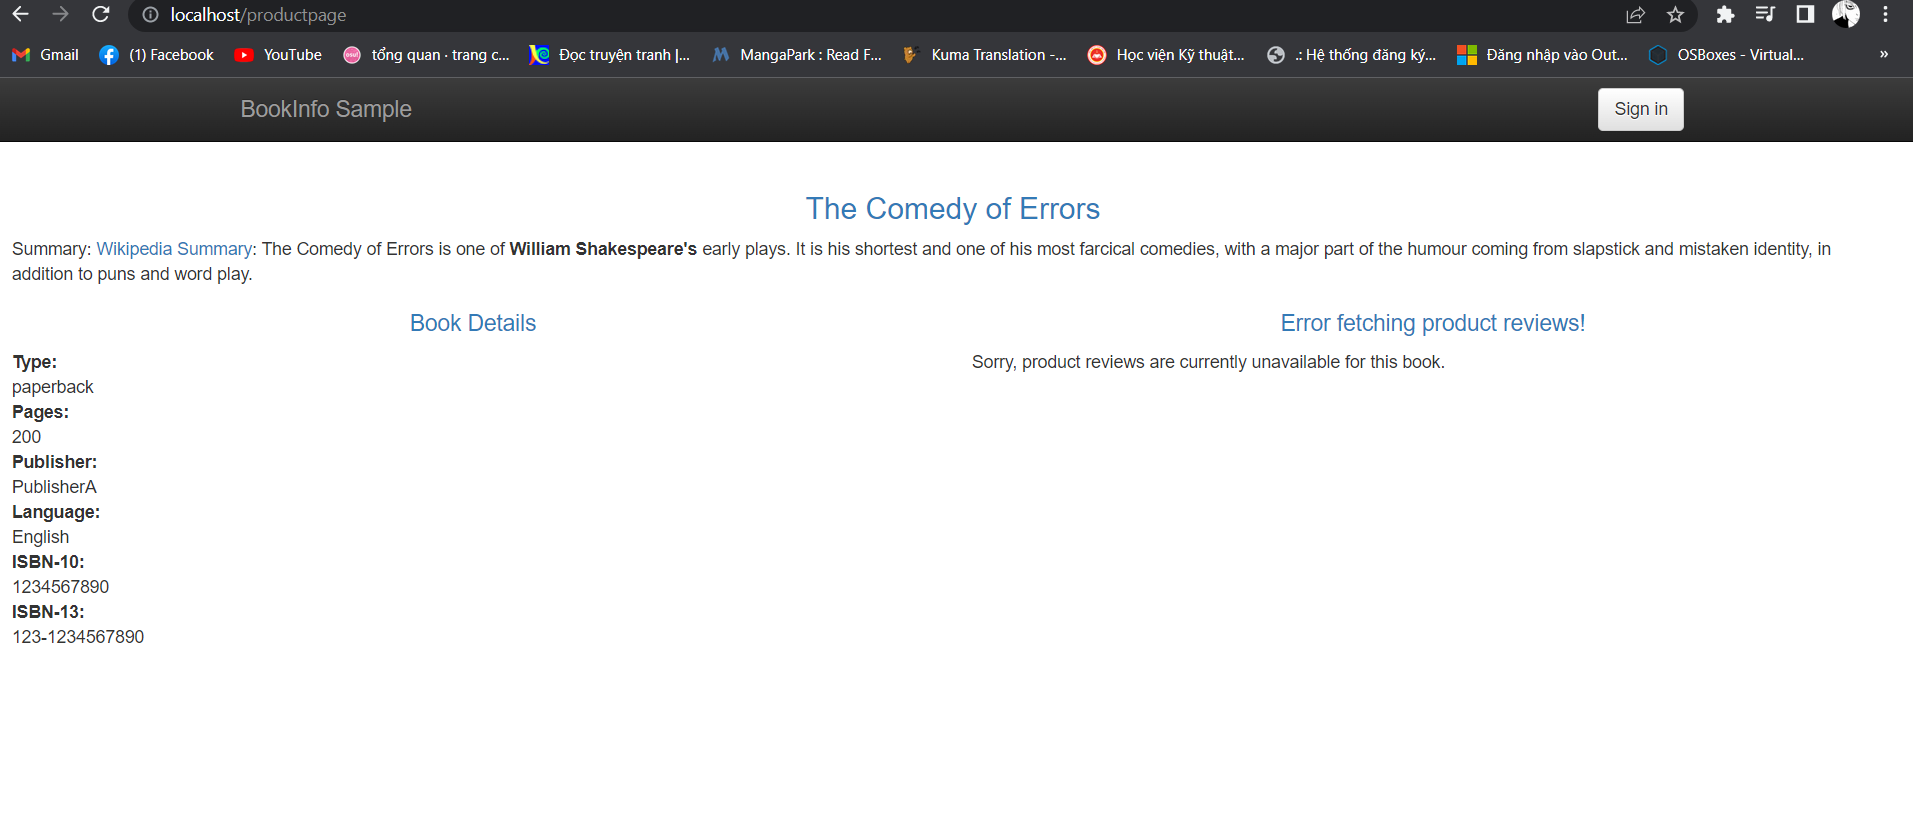
\includegraphics[width=0.7\linewidth]{Pics/3.3.2-p3}
					\caption{Dịch vụ details đã hoạt động như rating và reviews thì vẫn bị lỗi}
					\label{fig:3}
				\end{figure}

				Bước 7: Tạo file chính sách tương tự với dịch vụ rating và reviews xong đó dùng câu lệnh dưới để áp dụng file chính sách và vào lại trang dịch vụ trên trình duyệt:
				\begin{lstlisting}
				$ kubectl apply -f manifests/authoriztion/allow-rating.yaml 
				authorizationpolicy.security.istio.io/ratings-viewer created
				$ kubectl apply -f manifests/authoriztion/allow-reviews.yaml 
				authorizationpolicy.security.istio.io/reviews-viewer created
				\end{lstlisting}
				\begin{figure}[h]
					\centering
					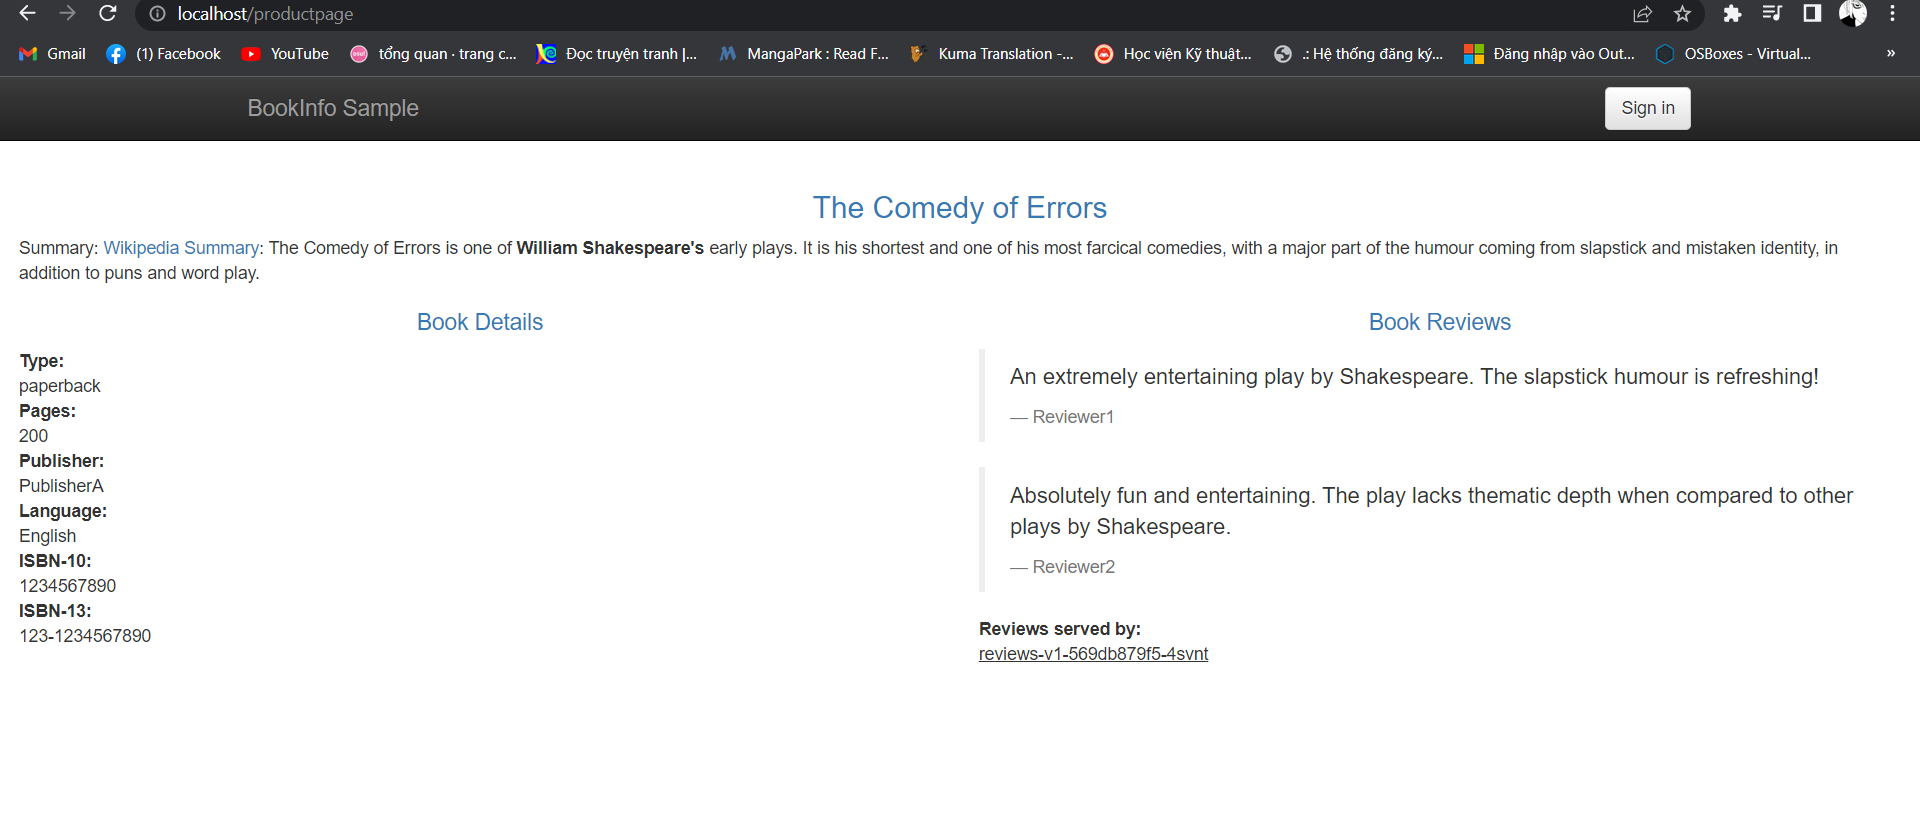
\includegraphics[width=0.7\linewidth]{Pics/3.3.2-p4}
					\caption{Các dịch vụ đều hoạt động bình thường}
					\label{fig:3}
				\end{figure}
		\pagebreak
		\section*{Kết luận chương 3}
		{\hspace{0.6cm}Qua phần thực nghiệm trên, cho thấy việc triển khai Istio là cực kì hữu dụng và quan trọng đối với bất kì hệ thống nào có sử dụng Kubernetes. Có thể sử dụng nhiều chiến lược triển khai như canary deployment, dark release, ...để có thể kiểm thử khi dịch vụ mới được triển khai có thể cho phép một lượng ít người dùng sử dụng tính năng để xem tính năng có bị lỗi hay không, hoặc chỉ có một nhóm người có thể sử dụng tính năng như các kĩ sư phần mềm hoặc các tester khi kiểm tra các tính năng mới của dịch vụ, và có thể quay về bản cũ nếu như tính năng mới của dịch vụ bị lỗi mà không làm ảnh hưởng gì đến hệ thống.}
		
		Khi các dịch vụ ngày càng phức tạp, việc hiểu hành vi và hiệu suất của hệ thống trở nên ngày càng khó khăn. Istio tạo phép đo từ xa chi tiết cho tất cả các thông tin liên lạc trong các dịch vụ. Phép đo từ xa này cung cấp khả năng quan sát hành vi dịch vụ, làm cho việc khắc phục sự cố, bảo trì và tối ưu hóa ứng dụng trở nên dễ dàng. Ngoài ra Istio còn hỗ trợ các phần mềm khác như kiali, prometheus, jaeger, grafana, ... tạo ra các biểu đồ thể hiện hiệu suất của hệ thống làm cho người quản trị viên có thể dễ dàng quản lí tập trung các microservice.
		
		Microservices có các nhu cầu bảo mật cụ thể, bao gồm bảo vệ chống lại các cuộc tấn công trung gian, kiểm soát truy cập linh hoạt, công cụ kiểm toán và xác thực giữa các microservice(mTLS). Istio bao gồm các giải pháp bảo mật toàn diện để cung cấp cho người vận hành khả năng giải quyết tất cả các vấn đề này. Nó cung cấp tính năng xác thực, ủy quyền, kiếm toán.
\chapter*{\centering Kết luận}
\addcontentsline{toc}{chapter}{Kết luận}

	Hầu hết các hệ thống hiện này đều sử dụng cấu trúc microservice, với cấu trúc này thì các nhà phát triển sẽ chỉ cần làm tốt phần công việc của họ, sau đó sẽ được liên kết với các tính năng hay ứng dụng khác thông qua API, các tính năng hay ứng dụng có thể nằm trong cùng một Pod hoặc khác Pod nhau nhưng với điều kiện các Pod này phải được giao tiếp với nhau, với việc các ứng dụng giao tiếp với bên ngoài nên việc bảo mật điều tất yếu. Thông qua báo cáo này, ta thấy rất rõ việc áp dụng các dịch vụ đảm bảo an toàn cho Pod là hiển nhiên và bắt buộc phải có, nếu muốn có một hệ thống an toàn hơn bằng cách hạn chế hoặc chặn quyền truy cập đến một số tài nguyên được xác định. Các dịch vụ này tương đối dễ tạo và triển khai và là thành phần hữu ích cho bất kỳ kế hoạch đảm bảo bảo mật cho Kubernetes.

	\begin{description}
		\item[Chương 1] đã nêu rõ được khái quát về cấu trúc các thành phần vận hành bên trong Container Kubernetes, Qua việc hiểu tổng quan của các công nghệ trênnhóm đã nhận ra một số vấn đề bảo mật của kiến trúc Microservices như nguy cơ bị tấn công cao khi mở rộng, việc ảnh hưởng đến hiệu suất khi triển khai bảo mật phân tán cũng như sự phức tạp, khó khăn khi triển khai các giải pháp an toàn cũng yêu cầu nhiều kiến thức đối với những nhà phát triển.
		\item[Chương 2] đã đi sâu sâu vào chi tiết về các tập hợp vi dịch vụ phân tán, các lớp cơ sở hạ tầng chuyên dụng như Service-mesh, quá trình triển khia các dịch vụ phân tán cũng như giao tiếp giữa dịch vụ với dịch vụ. Từ đó cho thấy Istio như một cách để giải quyết các bài toán gặp phải khi sử dụng các dịch vụ trên.
		\item[Chương 3] đã cho thấy việc triển khai Istio là cực kì hữu dụng và quan trọng đối với bất kì hệ thống nào có sử dụng Kubernetes. Có thể sử dụng nhiều chiến lược triển khai như canary deployment, dark release, ... Cung cấp khả năng quan sát hành vi dịch vụ, làm cho việc khắc phục sự cố, bảo trì và tối ưu hóa ứng dụng trở nên dễ dàng cũng như hỗ trợ các phần mềm theo dõi trực quan như kiali, jeager, grafane, v.v.. đồng thời bao gồm các giải pháp bảo mật toàn diện như các tính năng xác thực, ủy quyền, kiếm toán.
	\end{description}


\begin{thebibliography}{9}
\addcontentsline{toc}{chapter}{Tài liệu tham khảo}
	\bibitem{Kubernetes in Action Second Edition}
	Marko Luksa. Kubernetes in Action Second Edition MEAP V05 
	
	\bibitem{Istio in Action-Manning Publication}
	Christian E. Posta and Rinor Maloku. Istio in Action-Manning Publication
	
	\bibitem{Kubernetes Documentation}
	Kubernetes Documentation{https://kubernetes.io/docs/home/}
	
	\bibitem{Istio Documentation}
	Istio Documentation{https://istio.io/latest/docs/}
	
	\bibitem{Envoy Proxy Documentation}
	Envoy Proxy Documentation{https://www.envoyproxy.io/docs/}
\end{thebibliography}

\appendix 
\addcontentsline{toc}{chapter}{Phụ Lục}
\chapter{Các file cấu hình}
1. File cấu hình cấu hình bookinfo.yaml
\begin{lstlisting}
	# Copyright Istio Authors
	#
	#   Licensed under the Apache License, Version 2.0 (the "License");
	#   you may not use this file except in compliance with the License.
	#   You may obtain a copy of the License at
	#
	#       http://www.apache.org/licenses/LICENSE-2.0
	#
	#   Unless required by applicable law or agreed to in writing, software
	#   distributed under the License is distributed on an "AS IS" BASIS,
	#   WITHOUT WARRANTIES OR CONDITIONS OF ANY KIND, either express or implied.
	#   See the License for the specific language governing permissions and
	#   limitations under the License.
	
	####################################################
	# This file defines the services, service accounts, and deployments for the Bookinfo sample.
	#
	# To apply all 4 Bookinfo services, their corresponding service accounts, and deployments:
	#
	#   kubectl apply -f samples/bookinfo/platform/kube/bookinfo.yaml
	#
	# Alternatively, you can deploy any resource separately:
	#
	#   kubectl apply -f samples/bookinfo/platform/kube/bookinfo.yaml -l service=reviews # reviews Service
	#   kubectl apply -f samples/bookinfo/platform/kube/bookinfo.yaml -l account=reviews # reviews ServiceAccount
	#   kubectl apply -f samples/bookinfo/platform/kube/bookinfo.yaml -l app=reviews,version=v3 # reviews-v3 Deployment
	####################################################
	
	#################################
	# Details service
	#################################
	apiVersion: v1
	kind: Service
	metadata:
	  name: details
	  labels:
		app: details
		service: details
	spec:
	  ports:
	  - port: 9080
		name: http
	  selector:
		app: details
	---
	apiVersion: v1
	kind: ServiceAccount
	metadata:
	  name: bookinfo-details
	  labels:
		account: details
	---
	apiVersion: apps/v1
	kind: Deployment
	metadata:
	  name: details-v1
	  labels:
		app: details
		version: v1
	spec:
	  replicas: 1
	  selector:
		matchLabels:
		  app: details
		  version: v1
	  template:
		metadata:
		  labels:
			app: details
			version: v1
		spec:
		  serviceAccountName: bookinfo-details
		  containers:
		  - name: details
			image: docker.io/istio/examples-bookinfo-details-v1:1.17.0
			imagePullPolicy: IfNotPresent
			ports:
			- containerPort: 9080
			securityContext:
			  runAsUser: 1000
	---
	##################################################
	# Ratings service
	##################################################
	apiVersion: v1
	kind: Service
	metadata:
	  name: ratings
	  labels:
		app: ratings
		service: ratings
	spec:
	  ports:
	  - port: 9080
		name: http
	  selector:
		app: ratings
	---
	apiVersion: v1
	kind: ServiceAccount
	metadata:
	  name: bookinfo-ratings
	  labels:
		account: ratings
	---
	apiVersion: apps/v1
	kind: Deployment
	metadata:
	  name: ratings-v1
	  labels:
		app: ratings
		version: v1
	spec:
	  replicas: 1
	  selector:
		matchLabels:
		  app: ratings
		  version: v1
	  template:
		metadata:
		  labels:
			app: ratings
			version: v1
		spec:
		  serviceAccountName: bookinfo-ratings
		  containers:
		  - name: ratings
			image: docker.io/istio/examples-bookinfo-ratings-v1:1.17.0
			imagePullPolicy: IfNotPresent
			ports:
			- containerPort: 9080
			securityContext:
			  runAsUser: 1000
	---
	##########################################
	# Reviews service
	##########################################
	apiVersion: v1
	kind: Service
	metadata:
	  name: reviews
	  labels:
		app: reviews
		service: reviews
	spec:
	  ports:
	  - port: 9080
		name: http
	  selector:
		app: reviews
	---
	apiVersion: v1
	kind: ServiceAccount
	metadata:
	  name: bookinfo-reviews
	  labels:
		account: reviews
	---
	apiVersion: apps/v1
	kind: Deployment
	metadata:
	  name: reviews-v1
	  labels:
		app: reviews
		version: v1
	spec:
	  replicas: 1
	  selector:
		matchLabels:
		  app: reviews
		  version: v1
	  template:
		metadata:
		  labels:
			app: reviews
			version: v1
		spec:
		  serviceAccountName: bookinfo-reviews
		  containers:
		  - name: reviews
			image: docker.io/istio/examples-bookinfo-reviews-v1:1.17.0
			imagePullPolicy: IfNotPresent
			env:
			- name: LOG_DIR
			  value: "/tmp/logs"
			ports:
			- containerPort: 9080
			volumeMounts:
			- name: tmp
			  mountPath: /tmp
			- name: wlp-output
			  mountPath: /opt/ibm/wlp/output
			securityContext:
			  runAsUser: 1000
		  volumes:
		  - name: wlp-output
			emptyDir: {}
		  - name: tmp
			emptyDir: {}
	---
	apiVersion: apps/v1
	kind: Deployment
	metadata:
	  name: reviews-v2
	  labels:
		app: reviews
		version: v2
	spec:
	  replicas: 1
	  selector:
		matchLabels:
		  app: reviews
		  version: v2
	  template:
		metadata:
		  labels:
			app: reviews
			version: v2
		spec:
		  serviceAccountName: bookinfo-reviews
		  containers:
		  - name: reviews
			image: docker.io/istio/examples-bookinfo-reviews-v2:1.17.0
			imagePullPolicy: IfNotPresent
			env:
			- name: LOG_DIR
			  value: "/tmp/logs"
			ports:
			- containerPort: 9080
			volumeMounts:
			- name: tmp
			  mountPath: /tmp
			- name: wlp-output
			  mountPath: /opt/ibm/wlp/output
			securityContext:
			  runAsUser: 1000
		  volumes:
		  - name: wlp-output
			emptyDir: {}
		  - name: tmp
			emptyDir: {}
	---
	apiVersion: apps/v1
	kind: Deployment
	metadata:
	  name: reviews-v3
	  labels:
		app: reviews
		version: v3
	spec:
	  replicas: 1
	  selector:
		matchLabels:
		  app: reviews
		  version: v3
	  template:
		metadata:
		  labels:
			app: reviews
			version: v3
		spec:
		  serviceAccountName: bookinfo-reviews
		  containers:
		  - name: reviews
			image: docker.io/istio/examples-bookinfo-reviews-v3:1.17.0
			imagePullPolicy: IfNotPresent
			env:
			- name: LOG_DIR
			  value: "/tmp/logs"
			ports:
			- containerPort: 9080
			volumeMounts:
			- name: tmp
			  mountPath: /tmp
			- name: wlp-output
			  mountPath: /opt/ibm/wlp/output
			securityContext:
			  runAsUser: 1000
		  volumes:
		  - name: wlp-output
			emptyDir: {}
		  - name: tmp
			emptyDir: {}
	---
	################################
	# Productpage services
	################################
	apiVersion: v1
	kind: Service
	metadata:
	  name: productpage
	  labels:
		app: productpage
		service: productpage
	spec:
	  ports:
	  - port: 9080
		name: http
	  selector:
		app: productpage
	---
	apiVersion: v1
	kind: ServiceAccount
	metadata:
	  name: bookinfo-productpage
	  labels:
		account: productpage
	---
	apiVersion: apps/v1
	kind: Deployment
	metadata:
	  name: productpage-v1
	  labels:
		app: productpage
		version: v1
	spec:
	  replicas: 1
	  selector:
		matchLabels:
		  app: productpage
		  version: v1
	  template:
		metadata:
		  labels:
			app: productpage
			version: v1
		spec:
		  serviceAccountName: bookinfo-productpage
		  containers:
		  - name: productpage
			image: docker.io/istio/examples-bookinfo-productpage-v1:1.17.0
			imagePullPolicy: IfNotPresent
			ports:
			- containerPort: 9080
			volumeMounts:
			- name: tmp
			  mountPath: /tmp
			securityContext:
			  runAsUser: 1000
		  volumes:
		  - name: tmp
			emptyDir: {}
	---
\end{lstlisting}

2. File cấu hình bookinfo-gateway.yaml
\begin{lstlisting}
	apiVersion: networking.istio.io/v1alpha3
	kind: Gateway
	metadata:
	  name: bookinfo-gateway
	spec:
	  selector:
		istio: ingressgateway # use istio default controller
	  servers:
	  - port:
		  number: 80
		  name: http
		  protocol: HTTP
		hosts:
		- "*"
	---
	apiVersion: networking.istio.io/v1alpha3
	kind: VirtualService
	metadata:
	  name: bookinfo
	spec:
	  hosts:
	  - "*"
	  gateways:
	  - bookinfo-gateway
	  http:
	  - match:
		- uri:
			exact: /productpage
		- uri:
			prefix: /static
		- uri:
			exact: /login
		- uri:
			exact: /logout
		- uri:
			prefix: /api/v1/products
		route:
		- destination:
			host: productpage
			port:
			  number: 9080
	
\end{lstlisting}

3. File cấu hình destination-rule-all.yaml
\begin{lstlisting}
	apiVersion: networking.istio.io/v1alpha3
	kind: DestinationRule
	metadata:
	  name: productpage
	spec:
	  host: productpage
	  subsets:
	  - name: v1
		labels:
		  version: v1
	---
	apiVersion: networking.istio.io/v1alpha3
	kind: DestinationRule
	metadata:
	  name: reviews
	spec:
	  host: reviews
	  subsets:
	  - name: v1
		labels:
		  version: v1
	  - name: v2
		labels:
		  version: v2
	  - name: v3
		labels:
		  version: v3
	---
	apiVersion: networking.istio.io/v1alpha3
	kind: DestinationRule
	metadata:
	  name: ratings
	spec:
	  host: ratings
	  subsets:
	  - name: v1
		labels:
		  version: v1
	  - name: v2
		labels:
		  version: v2
	  - name: v2-mysql
		labels:
		  version: v2-mysql
	  - name: v2-mysql-vm
		labels:
		  version: v2-mysql-vm
	---
	apiVersion: networking.istio.io/v1alpha3
	kind: DestinationRule
	metadata:
	  name: details
	spec:
	  host: details
	  subsets:
	  - name: v1
		labels:
		  version: v1
	  - name: v2
		labels:
		  version: v2
	---
	
\end{lstlisting}

4. File cấu hình virtual-service-all-v1.yaml
\begin{lstlisting}
	apiVersion: networking.istio.io/v1alpha3
	kind: VirtualService
	metadata:
	  name: productpage
	spec:
	  hosts:
	  - productpage
	  http:
	  - route:
		- destination:
			host: productpage
			subset: v1
	---
	apiVersion: networking.istio.io/v1alpha3
	kind: VirtualService
	metadata:
	  name: reviews
	spec:
	  hosts:
	  - reviews
	  http:
	  - route:
		- destination:
			host: reviews
			subset: v1
	---
	apiVersion: networking.istio.io/v1alpha3
	kind: VirtualService
	metadata:
	  name: ratings
	spec:
	  hosts:
	  - ratings
	  http:
	  - route:
		- destination:
			host: ratings
			subset: v1
	---
	apiVersion: networking.istio.io/v1alpha3
	kind: VirtualService
	metadata:
	  name: details
	spec:
	  hosts:
	  - details
	  http:
	  - route:
		- destination:
			host: details
			subset: v1
	---
	
\end{lstlisting}

5. File cấu hình virtual-service-reviews-50-v3.yaml
\begin{lstlisting}
	apiVersion: networking.istio.io/v1alpha3
	kind: VirtualService
	metadata:
	  name: reviews
	spec:
	  hosts:
		- reviews
	  http:
	  - route:
		- destination:
			host: reviews
			subset: v1
		  weight: 50
		- destination:
			host: reviews
			subset: v3
		  weight: 50
	
\end{lstlisting}

6. File cấu hình virtual-service-reviews-80-20.yaml
\begin{lstlisting}
	apiVersion: networking.istio.io/v1alpha3
	kind: VirtualService
	metadata:
	  name: reviews
	spec:
	  hosts:
		- reviews
	  http:
	  - route:
		- destination:
			host: reviews
			subset: v1
		  weight: 80
		- destination:
			host: reviews
			subset: v2
		  weight: 20
	
\end{lstlisting}

7. File cấu hình virtual-service-reviews-90-10.yaml
\begin{lstlisting}
	apiVersion: networking.istio.io/v1alpha3
	kind: VirtualService
	metadata:
	  name: reviews
	spec:
	  hosts:
		- reviews
	  http:
	  - route:
		- destination:
			host: reviews
			subset: v1
		  weight: 90
		- destination:
			host: reviews
			subset: v2
		  weight: 10
	
\end{lstlisting}

8. File cấu hình kiali.yaml
\begin{lstlisting}
	---
	# Source: kiali-server/templates/serviceaccount.yaml
	apiVersion: v1
	kind: ServiceAccount
	metadata:
	  name: kiali
	  namespace: istio-system
	  labels:
		helm.sh/chart: kiali-server-1.55.1
		app: kiali
		app.kubernetes.io/name: kiali
		app.kubernetes.io/instance: kiali
		version: "v1.55.1"
		app.kubernetes.io/version: "v1.55.1"
		app.kubernetes.io/managed-by: Helm
		app.kubernetes.io/part-of: "kiali"
	...
	---
	# Source: kiali-server/templates/configmap.yaml
	apiVersion: v1
	kind: ConfigMap
	metadata:
	  name: kiali
	  namespace: istio-system
	  labels:
		helm.sh/chart: kiali-server-1.55.1
		app: kiali
		app.kubernetes.io/name: kiali
		app.kubernetes.io/instance: kiali
		version: "v1.55.1"
		app.kubernetes.io/version: "v1.55.1"
		app.kubernetes.io/managed-by: Helm
		app.kubernetes.io/part-of: "kiali"
	data:
	  config.yaml: |
		auth:
		  openid: {}
		  openshift:
			client_id_prefix: kiali
		  strategy: anonymous
		deployment:
		  accessible_namespaces:
		  - '**'
		  additional_service_yaml: {}
		  affinity:
			node: {}
			pod: {}
			pod_anti: {}
		  configmap_annotations: {}
		  custom_secrets: []
		  host_aliases: []
		  hpa:
			api_version: autoscaling/v2beta2
			spec: {}
		  image_digest: ""
		  image_name: quay.io/kiali/kiali
		  image_pull_policy: Always
		  image_pull_secrets: []
		  image_version: v1.55
		  ingress:
			additional_labels: {}
			class_name: nginx
			override_yaml:
			  metadata: {}
		  ingress_enabled: false
		  instance_name: kiali
		  logger:
			log_format: text
			log_level: info
			sampler_rate: "1"
			time_field_format: 2006-01-02T15:04:05Z07:00
		  namespace: istio-system
		  node_selector: {}
		  pod_annotations: {}
		  pod_labels:
			sidecar.istio.io/inject: "false"
		  priority_class_name: ""
		  replicas: 1
		  resources:
			limits:
			  memory: 1Gi
			requests:
			  cpu: 10m
			  memory: 64Mi
		  secret_name: kiali
		  service_annotations: {}
		  service_type: ""
		  tolerations: []
		  version_label: v1.55.1
		  view_only_mode: false
		external_services:
		  custom_dashboards:
			enabled: true
		  istio:
			root_namespace: istio-system
		identity:
		  cert_file: ""
		  private_key_file: ""
		istio_namespace: istio-system
		kiali_feature_flags:
		  certificates_information_indicators:
			enabled: true
			secrets:
			- cacerts
			- istio-ca-secret
		  clustering:
			enabled: true
		  disabled_features: []
		  validations:
			ignore:
			- KIA1201
		login_token:
		  signing_key: CHANGEME00000000
		server:
		  metrics_enabled: true
		  metrics_port: 9090
		  port: 20001
		  web_root: /kiali
	...
	---
	# Source: kiali-server/templates/role-viewer.yaml
	apiVersion: rbac.authorization.k8s.io/v1
	kind: ClusterRole
	metadata:
	  name: kiali-viewer
	  labels:
		helm.sh/chart: kiali-server-1.55.1
		app: kiali
		app.kubernetes.io/name: kiali
		app.kubernetes.io/instance: kiali
		version: "v1.55.1"
		app.kubernetes.io/version: "v1.55.1"
		app.kubernetes.io/managed-by: Helm
		app.kubernetes.io/part-of: "kiali"
	rules:
	- apiGroups: [""]
	  resources:
	  - configmaps
	  - endpoints
	  - pods/log
	  verbs:
	  - get
	  - list
	  - watch
	- apiGroups: [""]
	  resources:
	  - namespaces
	  - pods
	  - replicationcontrollers
	  - services
	  verbs:
	  - get
	  - list
	  - watch
	- apiGroups: [""]
	  resources:
	  - pods/portforward
	  verbs:
	  - create
	  - post
	- apiGroups: ["extensions", "apps"]
	  resources:
	  - daemonsets
	  - deployments
	  - replicasets
	  - statefulsets
	  verbs:
	  - get
	  - list
	  - watch
	- apiGroups: ["batch"]
	  resources:
	  - cronjobs
	  - jobs
	  verbs:
	  - get
	  - list
	  - watch
	- apiGroups:
	  - networking.istio.io
	  - security.istio.io
	  resources: ["*"]
	  verbs:
	  - get
	  - list
	  - watch
	- apiGroups: ["apps.openshift.io"]
	  resources:
	  - deploymentconfigs
	  verbs:
	  - get
	  - list
	  - watch
	- apiGroups: ["project.openshift.io"]
	  resources:
	  - projects
	  verbs:
	  - get
	- apiGroups: ["route.openshift.io"]
	  resources:
	  - routes
	  verbs:
	  - get
	- apiGroups: ["authentication.k8s.io"]
	  resources:
	  - tokenreviews
	  verbs:
	  - create
	...
	---
	# Source: kiali-server/templates/role.yaml
	apiVersion: rbac.authorization.k8s.io/v1
	kind: ClusterRole
	metadata:
	  name: kiali
	  labels:
		helm.sh/chart: kiali-server-1.55.1
		app: kiali
		app.kubernetes.io/name: kiali
		app.kubernetes.io/instance: kiali
		version: "v1.55.1"
		app.kubernetes.io/version: "v1.55.1"
		app.kubernetes.io/managed-by: Helm
		app.kubernetes.io/part-of: "kiali"
	rules:
	- apiGroups: [""]
	  resources:
	  - configmaps
	  - endpoints
	  - pods/log
	  verbs:
	  - get
	  - list
	  - watch
	- apiGroups: [""]
	  resources:
	  - namespaces
	  - pods
	  - replicationcontrollers
	  - services
	  verbs:
	  - get
	  - list
	  - watch
	  - patch
	- apiGroups: [""]
	  resources:
	  - pods/portforward
	  verbs:
	  - create
	  - post
	- apiGroups: ["extensions", "apps"]
	  resources:
	  - daemonsets
	  - deployments
	  - replicasets
	  - statefulsets
	  verbs:
	  - get
	  - list
	  - watch
	  - patch
	- apiGroups: ["batch"]
	  resources:
	  - cronjobs
	  - jobs
	  verbs:
	  - get
	  - list
	  - watch
	  - patch
	- apiGroups:
	  - networking.istio.io
	  - security.istio.io
	  resources: ["*"]
	  verbs:
	  - get
	  - list
	  - watch
	  - create
	  - delete
	  - patch
	- apiGroups: ["apps.openshift.io"]
	  resources:
	  - deploymentconfigs
	  verbs:
	  - get
	  - list
	  - watch
	  - patch
	- apiGroups: ["project.openshift.io"]
	  resources:
	  - projects
	  verbs:
	  - get
	- apiGroups: ["route.openshift.io"]
	  resources:
	  - routes
	  verbs:
	  - get
	- apiGroups: ["authentication.k8s.io"]
	  resources:
	  - tokenreviews
	  verbs:
	  - create
	...
	---
	# Source: kiali-server/templates/rolebinding.yaml
	apiVersion: rbac.authorization.k8s.io/v1
	kind: ClusterRoleBinding
	metadata:
	  name: kiali
	  labels:
		helm.sh/chart: kiali-server-1.55.1
		app: kiali
		app.kubernetes.io/name: kiali
		app.kubernetes.io/instance: kiali
		version: "v1.55.1"
		app.kubernetes.io/version: "v1.55.1"
		app.kubernetes.io/managed-by: Helm
		app.kubernetes.io/part-of: "kiali"
	roleRef:
	  apiGroup: rbac.authorization.k8s.io
	  kind: ClusterRole
	  name: kiali
	subjects:
	- kind: ServiceAccount
	  name: kiali
	  namespace: istio-system
	...
	---
	# Source: kiali-server/templates/role-controlplane.yaml
	apiVersion: rbac.authorization.k8s.io/v1
	kind: Role
	metadata:
	  name: kiali-controlplane
	  namespace: istio-system
	  labels:
		helm.sh/chart: kiali-server-1.55.1
		app: kiali
		app.kubernetes.io/name: kiali
		app.kubernetes.io/instance: kiali
		version: "v1.55.1"
		app.kubernetes.io/version: "v1.55.1"
		app.kubernetes.io/managed-by: Helm
		app.kubernetes.io/part-of: "kiali"
	rules:
	- apiGroups: [""]
	  resources:
	  - secrets
	  verbs:
	  - list
	- apiGroups: [""]
	  resourceNames:
	  - cacerts
	  - istio-ca-secret
	  resources:
	  - secrets
	  verbs:
	  - get
	  - list
	  - watch
	...
	---
	# Source: kiali-server/templates/rolebinding-controlplane.yaml
	apiVersion: rbac.authorization.k8s.io/v1
	kind: RoleBinding
	metadata:
	  name: kiali-controlplane
	  namespace: istio-system
	  labels:
		helm.sh/chart: kiali-server-1.55.1
		app: kiali
		app.kubernetes.io/name: kiali
		app.kubernetes.io/instance: kiali
		version: "v1.55.1"
		app.kubernetes.io/version: "v1.55.1"
		app.kubernetes.io/managed-by: Helm
		app.kubernetes.io/part-of: "kiali"
	roleRef:
	  apiGroup: rbac.authorization.k8s.io
	  kind: Role
	  name: kiali-controlplane
	subjects:
	- kind: ServiceAccount
	  name: kiali
	  namespace: istio-system
	...
	---
	# Source: kiali-server/templates/service.yaml
	apiVersion: v1
	kind: Service
	metadata:
	  name: kiali
	  namespace: istio-system
	  labels:
		helm.sh/chart: kiali-server-1.55.1
		app: kiali
		app.kubernetes.io/name: kiali
		app.kubernetes.io/instance: kiali
		version: "v1.55.1"
		app.kubernetes.io/version: "v1.55.1"
		app.kubernetes.io/managed-by: Helm
		app.kubernetes.io/part-of: "kiali"
	  annotations:
	spec:
	  ports:
	  - name: http
		protocol: TCP
		port: 20001
	  - name: http-metrics
		protocol: TCP
		port: 9090
	  selector:
		app.kubernetes.io/name: kiali
		app.kubernetes.io/instance: kiali
	...
	---
	# Source: kiali-server/templates/deployment.yaml
	apiVersion: apps/v1
	kind: Deployment
	metadata:
	  name: kiali
	  namespace: istio-system
	  labels:
		helm.sh/chart: kiali-server-1.55.1
		app: kiali
		app.kubernetes.io/name: kiali
		app.kubernetes.io/instance: kiali
		version: "v1.55.1"
		app.kubernetes.io/version: "v1.55.1"
		app.kubernetes.io/managed-by: Helm
		app.kubernetes.io/part-of: "kiali"
	spec:
	  replicas: 1
	  selector:
		matchLabels:
		  app.kubernetes.io/name: kiali
		  app.kubernetes.io/instance: kiali
	  strategy:
		rollingUpdate:
		  maxSurge: 1
		  maxUnavailable: 1
		type: RollingUpdate
	  template:
		metadata:
		  name: kiali
		  labels:
			helm.sh/chart: kiali-server-1.55.1
			app: kiali
			app.kubernetes.io/name: kiali
			app.kubernetes.io/instance: kiali
			version: "v1.55.1"
			app.kubernetes.io/version: "v1.55.1"
			app.kubernetes.io/managed-by: Helm
			app.kubernetes.io/part-of: "kiali"
			sidecar.istio.io/inject: "false"
		  annotations:
			checksum/config: 39233dc06d242510c3d3371750a5e0aa9075ebee63db3d00790ec59ef1f55ee8
			prometheus.io/scrape: "true"
			prometheus.io/port: "9090"
			kiali.io/dashboards: go,kiali
		spec:
		  serviceAccountName: kiali
		  containers:
		  - image: "quay.io/kiali/kiali:v1.55"
			imagePullPolicy: Always
			name: kiali
			command:
			- "/opt/kiali/kiali"
			- "-config"
			- "/kiali-configuration/config.yaml"
			securityContext:
			  allowPrivilegeEscalation: false
			  privileged: false
			  readOnlyRootFilesystem: true
			  runAsNonRoot: true
			ports:
			- name: api-port
			  containerPort: 20001
			- name: http-metrics
			  containerPort: 9090
			readinessProbe:
			  httpGet:
				path: /kiali/healthz
				port: api-port
				scheme: HTTP
			  initialDelaySeconds: 5
			  periodSeconds: 30
			livenessProbe:
			  httpGet:
				path: /kiali/healthz
				port: api-port
				scheme: HTTP
			  initialDelaySeconds: 5
			  periodSeconds: 30
			env:
			- name: ACTIVE_NAMESPACE
			  valueFrom:
				fieldRef:
				  fieldPath: metadata.namespace
			- name: LOG_LEVEL
			  value: "info"
			- name: LOG_FORMAT
			  value: "text"
			- name: LOG_TIME_FIELD_FORMAT
			  value: "2006-01-02T15:04:05Z07:00"
			- name: LOG_SAMPLER_RATE
			  value: "1"
			volumeMounts:
			- name: kiali-configuration
			  mountPath: "/kiali-configuration"
			- name: kiali-cert
			  mountPath: "/kiali-cert"
			- name: kiali-secret
			  mountPath: "/kiali-secret"
			- name: kiali-cabundle
			  mountPath: "/kiali-cabundle"
			resources:
			  limits:
				memory: 1Gi
			  requests:
				cpu: 10m
				memory: 64Mi
		  volumes:
		  - name: kiali-configuration
			configMap:
			  name: kiali
		  - name: kiali-cert
			secret:
			  secretName: istio.kiali-service-account
			  optional: true
		  - name: kiali-secret
			secret:
			  secretName: kiali
			  optional: true
		  - name: kiali-cabundle
			configMap:
			  name: kiali-cabundle
			  optional: true
	...
	
\end{lstlisting}

9. File cấu hình prometheus.yaml
\begin{lstlisting}
	---
	# Source: prometheus/templates/server/serviceaccount.yaml
	apiVersion: v1
	kind: ServiceAccount
	metadata:
	  labels:
		component: "server"
		app: prometheus
		release: prometheus
		chart: prometheus-15.9.0
		heritage: Helm
	  name: prometheus
	  namespace: istio-system
	  annotations:
		{}
	---
	# Source: prometheus/templates/server/cm.yaml
	apiVersion: v1
	kind: ConfigMap
	metadata:
	  labels:
		component: "server"
		app: prometheus
		release: prometheus
		chart: prometheus-15.9.0
		heritage: Helm
	  name: prometheus
	  namespace: istio-system
	data:
	  alerting_rules.yml: |
		{}
	  alerts: |
		{}
	  prometheus.yml: |
		global:
		  evaluation_interval: 1m
		  scrape_interval: 15s
		  scrape_timeout: 10s
		rule_files:
		- /etc/config/recording_rules.yml
		- /etc/config/alerting_rules.yml
		- /etc/config/rules
		- /etc/config/alerts
		scrape_configs:
		- job_name: prometheus
		  static_configs:
		  - targets:
			- localhost:9090
		- bearer_token_file: /var/run/secrets/kubernetes.io/serviceaccount/token
		  job_name: kubernetes-apiservers
		  kubernetes_sd_configs:
		  - role: endpoints
		  relabel_configs:
		  - action: keep
			regex: default;kubernetes;https
			source_labels:
			- __meta_kubernetes_namespace
			- __meta_kubernetes_service_name
			- __meta_kubernetes_endpoint_port_name
		  scheme: https
		  tls_config:
			ca_file: /var/run/secrets/kubernetes.io/serviceaccount/ca.crt
			insecure_skip_verify: true
		- bearer_token_file: /var/run/secrets/kubernetes.io/serviceaccount/token
		  job_name: kubernetes-nodes
		  kubernetes_sd_configs:
		  - role: node
		  relabel_configs:
		  - action: labelmap
			regex: __meta_kubernetes_node_label_(.+)
		  - replacement: kubernetes.default.svc:443
			target_label: __address__
		  - regex: (.+)
			replacement: /api/v1/nodes/$1/proxy/metrics
			source_labels:
			- __meta_kubernetes_node_name
			target_label: __metrics_path__
		  scheme: https
		  tls_config:
			ca_file: /var/run/secrets/kubernetes.io/serviceaccount/ca.crt
			insecure_skip_verify: true
		- bearer_token_file: /var/run/secrets/kubernetes.io/serviceaccount/token
		  job_name: kubernetes-nodes-cadvisor
		  kubernetes_sd_configs:
		  - role: node
		  relabel_configs:
		  - action: labelmap
			regex: __meta_kubernetes_node_label_(.+)
		  - replacement: kubernetes.default.svc:443
			target_label: __address__
		  - regex: (.+)
			replacement: /api/v1/nodes/$1/proxy/metrics/cadvisor
			source_labels:
			- __meta_kubernetes_node_name
			target_label: __metrics_path__
		  scheme: https
		  tls_config:
			ca_file: /var/run/secrets/kubernetes.io/serviceaccount/ca.crt
			insecure_skip_verify: true
		- honor_labels: true
		  job_name: kubernetes-service-endpoints
		  kubernetes_sd_configs:
		  - role: endpoints
		  relabel_configs:
		  - action: keep
			regex: true
			source_labels:
			- __meta_kubernetes_service_annotation_prometheus_io_scrape
		  - action: drop
			regex: true
			source_labels:
			- __meta_kubernetes_service_annotation_prometheus_io_scrape_slow
		  - action: replace
			regex: (https?)
			source_labels:
			- __meta_kubernetes_service_annotation_prometheus_io_scheme
			target_label: __scheme__
		  - action: replace
			regex: (.+)
			source_labels:
			- __meta_kubernetes_service_annotation_prometheus_io_path
			target_label: __metrics_path__
		  - action: replace
			regex: ([^:]+)(?::\d+)?;(\d+)
			replacement: $1:$2
			source_labels:
			- __address__
			- __meta_kubernetes_service_annotation_prometheus_io_port
			target_label: __address__
		  - action: labelmap
			regex: __meta_kubernetes_service_annotation_prometheus_io_param_(.+)
			replacement: __param_$1
		  - action: labelmap
			regex: __meta_kubernetes_service_label_(.+)
		  - action: replace
			source_labels:
			- __meta_kubernetes_namespace
			target_label: namespace
		  - action: replace
			source_labels:
			- __meta_kubernetes_service_name
			target_label: service
		  - action: replace
			source_labels:
			- __meta_kubernetes_pod_node_name
			target_label: node
		- honor_labels: true
		  job_name: kubernetes-service-endpoints-slow
		  kubernetes_sd_configs:
		  - role: endpoints
		  relabel_configs:
		  - action: keep
			regex: true
			source_labels:
			- __meta_kubernetes_service_annotation_prometheus_io_scrape_slow
		  - action: replace
			regex: (https?)
			source_labels:
			- __meta_kubernetes_service_annotation_prometheus_io_scheme
			target_label: __scheme__
		  - action: replace
			regex: (.+)
			source_labels:
			- __meta_kubernetes_service_annotation_prometheus_io_path
			target_label: __metrics_path__
		  - action: replace
			regex: ([^:]+)(?::\d+)?;(\d+)
			replacement: $1:$2
			source_labels:
			- __address__
			- __meta_kubernetes_service_annotation_prometheus_io_port
			target_label: __address__
		  - action: labelmap
			regex: __meta_kubernetes_service_annotation_prometheus_io_param_(.+)
			replacement: __param_$1
		  - action: labelmap
			regex: __meta_kubernetes_service_label_(.+)
		  - action: replace
			source_labels:
			- __meta_kubernetes_namespace
			target_label: namespace
		  - action: replace
			source_labels:
			- __meta_kubernetes_service_name
			target_label: service
		  - action: replace
			source_labels:
			- __meta_kubernetes_pod_node_name
			target_label: node
		  scrape_interval: 5m
		  scrape_timeout: 30s
		- honor_labels: true
		  job_name: prometheus-pushgateway
		  kubernetes_sd_configs:
		  - role: service
		  relabel_configs:
		  - action: keep
			regex: pushgateway
			source_labels:
			- __meta_kubernetes_service_annotation_prometheus_io_probe
		- honor_labels: true
		  job_name: kubernetes-services
		  kubernetes_sd_configs:
		  - role: service
		  metrics_path: /probe
		  params:
			module:
			- http_2xx
		  relabel_configs:
		  - action: keep
			regex: true
			source_labels:
			- __meta_kubernetes_service_annotation_prometheus_io_probe
		  - source_labels:
			- __address__
			target_label: __param_target
		  - replacement: blackbox
			target_label: __address__
		  - source_labels:
			- __param_target
			target_label: instance
		  - action: labelmap
			regex: __meta_kubernetes_service_label_(.+)
		  - source_labels:
			- __meta_kubernetes_namespace
			target_label: namespace
		  - source_labels:
			- __meta_kubernetes_service_name
			target_label: service
		- honor_labels: true
		  job_name: kubernetes-pods
		  kubernetes_sd_configs:
		  - role: pod
		  relabel_configs:
		  - action: keep
			regex: true
			source_labels:
			- __meta_kubernetes_pod_annotation_prometheus_io_scrape
		  - action: drop
			regex: true
			source_labels:
			- __meta_kubernetes_pod_annotation_prometheus_io_scrape_slow
		  - action: replace
			regex: (https?)
			source_labels:
			- __meta_kubernetes_pod_annotation_prometheus_io_scheme
			target_label: __scheme__
		  - action: replace
			regex: (.+)
			source_labels:
			- __meta_kubernetes_pod_annotation_prometheus_io_path
			target_label: __metrics_path__
		  - action: replace
			regex: ([^:]+)(?::\d+)?;(\d+)
			replacement: $1:$2
			source_labels:
			- __address__
			- __meta_kubernetes_pod_annotation_prometheus_io_port
			target_label: __address__
		  - action: labelmap
			regex: __meta_kubernetes_pod_annotation_prometheus_io_param_(.+)
			replacement: __param_$1
		  - action: labelmap
			regex: __meta_kubernetes_pod_label_(.+)
		  - action: replace
			source_labels:
			- __meta_kubernetes_namespace
			target_label: namespace
		  - action: replace
			source_labels:
			- __meta_kubernetes_pod_name
			target_label: pod
		  - action: drop
			regex: Pending|Succeeded|Failed|Completed
			source_labels:
			- __meta_kubernetes_pod_phase
		- honor_labels: true
		  job_name: kubernetes-pods-slow
		  kubernetes_sd_configs:
		  - role: pod
		  relabel_configs:
		  - action: keep
			regex: true
			source_labels:
			- __meta_kubernetes_pod_annotation_prometheus_io_scrape_slow
		  - action: replace
			regex: (https?)
			source_labels:
			- __meta_kubernetes_pod_annotation_prometheus_io_scheme
			target_label: __scheme__
		  - action: replace
			regex: (.+)
			source_labels:
			- __meta_kubernetes_pod_annotation_prometheus_io_path
			target_label: __metrics_path__
		  - action: replace
			regex: ([^:]+)(?::\d+)?;(\d+)
			replacement: $1:$2
			source_labels:
			- __address__
			- __meta_kubernetes_pod_annotation_prometheus_io_port
			target_label: __address__
		  - action: labelmap
			regex: __meta_kubernetes_pod_annotation_prometheus_io_param_(.+)
			replacement: __param_$1
		  - action: labelmap
			regex: __meta_kubernetes_pod_label_(.+)
		  - action: replace
			source_labels:
			- __meta_kubernetes_namespace
			target_label: namespace
		  - action: replace
			source_labels:
			- __meta_kubernetes_pod_name
			target_label: pod
		  - action: drop
			regex: Pending|Succeeded|Failed|Completed
			source_labels:
			- __meta_kubernetes_pod_phase
		  scrape_interval: 5m
		  scrape_timeout: 30s
	  recording_rules.yml: |
		{}
	  rules: |
		{}
	---
	# Source: prometheus/templates/server/clusterrole.yaml
	apiVersion: rbac.authorization.k8s.io/v1
	kind: ClusterRole
	metadata:
	  labels:
		component: "server"
		app: prometheus
		release: prometheus
		chart: prometheus-15.9.0
		heritage: Helm
	  name: prometheus
	rules:
	  - apiGroups:
		  - ""
		resources:
		  - nodes
		  - nodes/proxy
		  - nodes/metrics
		  - services
		  - endpoints
		  - pods
		  - ingresses
		  - configmaps
		verbs:
		  - get
		  - list
		  - watch
	  - apiGroups:
		  - "extensions"
		  - "networking.k8s.io"
		resources:
		  - ingresses/status
		  - ingresses
		verbs:
		  - get
		  - list
		  - watch
	  - nonResourceURLs:
		  - "/metrics"
		verbs:
		  - get
	---
	# Source: prometheus/templates/server/clusterrolebinding.yaml
	apiVersion: rbac.authorization.k8s.io/v1
	kind: ClusterRoleBinding
	metadata:
	  labels:
		component: "server"
		app: prometheus
		release: prometheus
		chart: prometheus-15.9.0
		heritage: Helm
	  name: prometheus
	subjects:
	  - kind: ServiceAccount
		name: prometheus
		namespace: istio-system
	roleRef:
	  apiGroup: rbac.authorization.k8s.io
	  kind: ClusterRole
	  name: prometheus
	---
	# Source: prometheus/templates/server/service.yaml
	apiVersion: v1
	kind: Service
	metadata:
	  labels:
		component: "server"
		app: prometheus
		release: prometheus
		chart: prometheus-15.9.0
		heritage: Helm
	  name: prometheus
	  namespace: istio-system
	spec:
	  ports:
		- name: http
		  port: 9090
		  protocol: TCP
		  targetPort: 9090
	  selector:
		component: "server"
		app: prometheus
		release: prometheus
	  sessionAffinity: None
	  type: "ClusterIP"
	---
	# Source: prometheus/templates/server/deploy.yaml
	apiVersion: apps/v1
	kind: Deployment
	metadata:
	  labels:
		component: "server"
		app: prometheus
		release: prometheus
		chart: prometheus-15.9.0
		heritage: Helm
	  name: prometheus
	  namespace: istio-system
	spec:
	  selector:
		matchLabels:
		  component: "server"
		  app: prometheus
		  release: prometheus
	  replicas: 1
	  template:
		metadata:
		  labels:
			component: "server"
			app: prometheus
			release: prometheus
			chart: prometheus-15.9.0
			heritage: Helm
			
			sidecar.istio.io/inject: "false"
		spec:
		  enableServiceLinks: true
		  serviceAccountName: prometheus
		  containers:
			- name: prometheus-server-configmap-reload
			  image: "jimmidyson/configmap-reload:v0.5.0"
			  imagePullPolicy: "IfNotPresent"
			  args:
				- --volume-dir=/etc/config
				- --webhook-url=http://127.0.0.1:9090/-/reload
			  resources:
				{}
			  volumeMounts:
				- name: config-volume
				  mountPath: /etc/config
				  readOnly: true
	
			- name: prometheus-server
			  image: "prom/prometheus:v2.34.0"
			  imagePullPolicy: "IfNotPresent"
			  args:
				- --storage.tsdb.retention.time=15d
				- --config.file=/etc/config/prometheus.yml
				- --storage.tsdb.path=/data
				- --web.console.libraries=/etc/prometheus/console_libraries
				- --web.console.templates=/etc/prometheus/consoles
				- --web.enable-lifecycle
			  ports:
				- containerPort: 9090
			  readinessProbe:
				httpGet:
				  path: /-/ready
				  port: 9090
				  scheme: HTTP
				initialDelaySeconds: 0
				periodSeconds: 5
				timeoutSeconds: 4
				failureThreshold: 3
				successThreshold: 1
			  livenessProbe:
				httpGet:
				  path: /-/healthy
				  port: 9090
				  scheme: HTTP
				initialDelaySeconds: 30
				periodSeconds: 15
				timeoutSeconds: 10
				failureThreshold: 3
				successThreshold: 1
			  resources:
				{}
			  volumeMounts:
				- name: config-volume
				  mountPath: /etc/config
				- name: storage-volume
				  mountPath: /data
				  subPath: ""
		  hostNetwork: false
		  dnsPolicy: ClusterFirst
		  securityContext:
			fsGroup: 65534
			runAsGroup: 65534
			runAsNonRoot: true
			runAsUser: 65534
		  terminationGracePeriodSeconds: 300
		  volumes:
			- name: config-volume
			  configMap:
				name: prometheus
			- name: storage-volume
			  emptyDir:
				{}
	
\end{lstlisting}

10. File cấu hình allow-details.yaml
\begin{lstlisting}
	apiVersion: security.istio.io/v1beta1
	kind: AuthorizationPolicy
	metadata:
	  name: "details-viewer"
	  namespace: default
	spec:
	  selector:
		matchLabels:
		  app: details
	  action: ALLOW
	  rules:
	  - from:
		- source:
			principals: ["cluster.local/ns/default/sa/bookinfo-productpage"]
		to:
		- operation:
			methods: ["GET"]
\end{lstlisting}

11. File cấu hình allow-product-page.yaml
\begin{lstlisting}
	apiVersion: security.istio.io/v1beta1
	kind: AuthorizationPolicy
	metadata:
	  name: "productpage-viewer"
	  namespace: default
	spec:
	  selector:
		matchLabels:
		  app: productpage
	  action: ALLOW
	  rules:
	  - to:
		- operation:
			methods: ["GET"]
\end{lstlisting}

12. File cấu hình allow-rating.yaml
\begin{lstlisting}
	apiVersion: security.istio.io/v1beta1
	kind: AuthorizationPolicy
	metadata:
	  name: "ratings-viewer"
	  namespace: default
	spec:
	  selector:
		matchLabels:
		  app: ratings
	  action: ALLOW
	  rules:
	  - from:
		- source:
			principals: ["cluster.local/ns/default/sa/bookinfo-reviews"]
		to:
		- operation:
			methods: ["GET"]
\end{lstlisting}

13. File cấu hình allow-reviews.yaml
\begin{lstlisting}
	apiVersion: security.istio.io/v1beta1
	kind: AuthorizationPolicy
	metadata:
	  name: "reviews-viewer"
	  namespace: default
	spec:
	  selector:
		matchLabels:
		  app: reviews
	  action: ALLOW
	  rules:
	  - from:
		- source:
			principals: ["cluster.local/ns/default/sa/bookinfo-productpage"]
		to:
		- operation:
			methods: ["GET"]
\end{lstlisting}

14. File cấu hình deny-all.yaml
\begin{lstlisting}
	apiVersion: security.istio.io/v1beta1
	kind: AuthorizationPolicy
	metadata:
	  name: allow-nothing
	  namespace: default
	spec:
	  {}
\end{lstlisting}

15. File cấu hình meshwide-strict-peer-authn.yaml
\begin{lstlisting}
	apiVersion: "security.istio.io/v1beta1"
	kind: "PeerAuthentication"
	metadata:
	  name: "default"
	  namespace: "istio-system"
	spec:
	  mtls:
		mode: STRICT 
	
\end{lstlisting}

16. File cấu hình sleep.yaml
\begin{lstlisting}
	apiVersion: v1
	kind: ServiceAccount
	metadata:
	  name: sleep
	---
	apiVersion: v1
	kind: Service
	metadata:
	  name: sleep
	  labels:
		app: sleep
	spec:
	  ports:
	  - port: 80
		name: http
	  selector:
		app: sleep
	---
	apiVersion: apps/v1
	kind: Deployment
	metadata:
	  name: sleep
	spec:
	  replicas: 1
	  selector:
		matchLabels:
		  app: sleep
	  template:
		metadata:
		  labels:
			app: sleep
		spec:
		  serviceAccountName: sleep
		  containers:
		  - name: sleep
			image: governmentpaas/curl-ssl
			command: ["/bin/sleep", "3650d"]
			imagePullPolicy: IfNotPresent
			volumeMounts:
			- mountPath: /etc/sleep/tls
			  name: secret-volume
		  volumes:
		  - name: secret-volume
			secret:
			  secretName: sleep-secret
			  optional: true
	---
\end{lstlisting}
\end{document}